
%parametros de tipo libro
\documentclass[10pt,a4paper]{book}

%idioma español y acentos
\usepackage[spanish, es-tabla]{babel}
%\usepackage[latin1]{inputenc}
\usepackage[utf8]{inputenc}
%algunos sÌmbolos matem·ticos y paquete para usar subim·genes
\usepackage{pdfpages}
\usepackage{amsfonts}
\usepackage{amssymb}
\usepackage{graphicx}
\usepackage{subfigure}
\usepackage{listings}
\usepackage{appendix}

\usepackage{amsmath}
\usepackage{booktabs}
\usepackage{lscape}
\usepackage{adjustbox}
\usepackage{algorithm} 
\usepackage{algorithmic} 
\usepackage{listings}
\usepackage{xcolor}  % Paquete para definir colores
\usepackage[left=3cm,top=3cm,right=3cm,bottom=3cm]{geometry}






\usepackage{fancyhdr}
\pagestyle{fancy}
\fancyhf{} % Limpia todas las cabeceras y pies de página

% Aumenta el espacio de la cabecera
\setlength{\headheight}{16pt} % Ajusta según sea necesario
\setlength{\headsep}{25pt} % Ajusta según sea necesario


% Configuración para las páginas impares (recto)
\fancyhead[RO]{\MakeUppercase{\rightmark}} % Número de sección y nombre de sección en la cabecera derecha
\fancyfoot[RO]{\thepage} % Número de página en el pie de página derecho

% Configuración para las páginas pares (verso)
\fancyhead[LE]{\MakeUppercase{\leftmark}} % Número de capítulo y nombre de capítulo en la cabecera izquierda
\fancyfoot[LE]{\thepage} % Número de página en el pie de página izquierdo

% Actualiza las marcas de capítulo y sección
\renewcommand{\chaptermark}[1]{\markboth{\thechapter\quad #1}{}}
\renewcommand{\sectionmark}[1]{\markright{\thesection\quad #1}}






%
\usepackage{multicol}

%para generar índice con hipervínculos
\usepackage{hyperref}

%parametros del documento (sus propiedades)
\hypersetup{
	pdftitle={Nombre del alumno - TFG - año},
	pdfsubject={TFG - año},
	pdfauthor={Nombre del alumno},
	pdfkeywords={palabraclave1} {palabraclave2} {palabraclave3},
	colorlinks,
	citecolor=black,
	filecolor=black,
	linkcolor=black,
	urlcolor=black,
}
% Configuración de \lstset para un código más estético
\lstset{
	language=Python,    
	basicstyle=\ttfamily\small,   
	keywordstyle=\color{blue}\bfseries,    
	commentstyle=\color{teal}\itshape,    
	stringstyle=\color{brown},          
	numberstyle=\tiny\color{gray},        
	numbers=left,                         
	stepnumber=1,                          
	numbersep=10pt,                        
	backgroundcolor=\color{lightgray!20},  
	showspaces=false,                       
	showstringspaces=false,                
	showtabs=false,                        
	frame=single,                           
	rulecolor=\color{black},                
	captionpos=b,                          
	breaklines=true,                      
	breakatwhitespace=true,               
	tabsize=4,                            
	escapeinside={\%*}{*)},               
	morekeywords={self},                  
	xleftmargin=15pt,                     
	xrightmargin=15pt                   
}


%M·rgenes


%empieza el documento
\begin{document}  

%elementos antes del trabajo en sÌ se meten dentro de frontmatter
\frontmatter

%cada incluye referencia a un archivo de tipo .tex
\begin{titlepage}
\begin{center}

%forma de introducir imágenes. el \\[0.5 cm] de final de línea introduce un salto de ese tamaño.
%width=1\textwidth indica el tamaño de la imágen (valores entre 0-1). 
 
\includegraphics[width=1\textwidth]{figuras/cabecera.png}  \\[0.5 cm]

\LARGE UNIVERSIDAD POLITÉCNICA DE MADRID \\ [1 cm]

\LARGE ESCUELA TÉCNICA SUPERIOR DE INGENIERÍA Y DISEÑO INDUSTRIAL \\ [1 cm]

\LARGE Grado en Ingeniería Electrónica y Automática Industrial\\ [1 cm]

\LARGE \textbf{TRABAJO FIN DE GRADO}\\[1 cm]

\Huge \textsc{Desarrollo de modelos de la progresión del declive cognitivo en pacientes con la enfermedad del Parkinson mediante Leaspy}\\[1 cm]

\LARGE Raquel Roca Pereira \\[1 cm]

%flushleft alinea a la izquierda el texto

\begin{flushleft} \Large
\emph{Tutor:} Carlos Platero Dueñas\\
\emph{Departamento:} : Ingeniería Eléctrica, Electrónica, Automática y Física Aplicada 
\end{flushleft}


%rellena de blanco el resto de la página para escribir abajo del todo
\vfill

% Bottom of the page
{\large Madrid, Septiembre, 2024}

%SE ponen al final firmas.tex
%\end{center}
%\end{titlepage}


\cleardoublepage 

%\begin{center}
% Está puesto en portada.tex
\thispagestyle{empty}
%forma de introducir imágenes. el \\[0.5 cm] de final de línea introduce un salto de ese tamaño.
%width=1\textwidth indica el tamaño de la imágen (valores entre 0-1). 

\includegraphics[width=1\textwidth]{figuras/cabecera.png}  \\[0.5 cm]

\LARGE UNIVERSIDAD POLITÉCNICA DE MADRID \\ [1 cm]

\LARGE ESCUELA TÉCNICA SUPERIOR DE INGENIERÍA Y DISEÑO INDUSTRIAL \\ [1 cm]

\LARGE Grado en Ingeniería Electrónica y Automática Industrial\\ [1 cm]

\LARGE \textbf{TRABAJO FIN DE GRADO}\\[1 cm]

\Huge \textsc{Desarrollo de modelos de la progresión del declive cognitivo en pacientes con la enfermedad del Parkinson mediante Leaspy}\\[2 cm]

\Large Firma Autor \\[3 cm]

%flushleft alinea a la izquierda el texto

\begin{multicols}{2} 
	\begin{flushleft} 
		\Large \emph{Firma Cotutor (si lo hay)}
	\end{flushleft}
	
	\begin{flushright} 
		\Large \emph{Firma Tutor}
	\end{flushright}
	
\end{multicols} 

%rellena de blanco el resto de la página para escribir abajo del todo
\vfill

\end{center}
\end{titlepage}


\cleardoublepage 

%Licencia opcional
\begin{flushleft}

Copyright \copyright  2024. Raquel Roca Pereira

%ejemplo de licencia, se puede elegir cualquier otra

Esta obra está licenciada bajo la licencia Creative Commons Atribución-NoComercial-SinDerivadas 3.0 Unported (CC BY-NC-ND 3.0). Para ver una copia de esta licencia, visite http://creativecommons.org/licenses/by-nc-nd/3.0/deed.es o envíe una carta a Creative Commons, 444 Castro Street, Suite 900, Mountain View, California, 94041, EE.UU.

Todas las opiniones aquí expresadas son del autor, y no reflejan necesariamente las opiniones
de la Universidad Politécnica de Madrid.

\end{flushleft}

\cleardoublepage

\begin{flushleft} \large
\textbf{TÌtulo:} {Desarrollo de modelos de la progresión del declive cognitivo en pacientes con la enfermedad del Parkinson mediante Leaspy} \\
\textbf{Autor:} Raquel Roca Pereira\\
\textbf{Tutor:} Carlos Platero Dueñas \\[1 cm]

\end{flushleft} 

\begin{center} \LARGE
EL TRIBUNAL \\ [1 cm]
\end{center}

\begin{flushleft} \LARGE
Presidente: \\ [1 cm]
Vocal: \\ [1 cm]
Secretario: \\ [1.5 cm]
\end{flushleft}

\large
Realizado el acto de defensa y lectura del Trabajo Fin de Grado el día ....... de ....................   de ... en .........., en la Escuela Técnica Superior de Ingeniería y Diseño Industrial de la Universidad Politécnica de Madrid, acuerda otorgarle la CALIFICACIÓN de: \\ [2 cm]

\begin{center}
 \large VOCAL \\ [2.2 cm]
\end{center}

\begin{minipage}{0.5\textwidth}
 \begin{flushleft}
 \large SECRETARIO
\end{flushleft}
\end{minipage}
\begin{minipage}{0.5\textwidth}
\begin{flushright}
 \large PRESIDENTE
\end{flushright} 
\end{minipage}

\chapter{Agradecimientos}
Primero de todo, me gustaría agradecer a mis padres y a mi hermano por el apoyo constante. Por recordarme que con esfuerzo se acaban logrando las cosas y por animarme a perseguir mis objetivos y hacer aquello que realmente me guste.\\

Agradecer también a Tesa, por todas las horas de biblioteca y de estudio infinitas pero, todavía más importante, por todos los momentos de cuidados y de alegrías. Por estar siempre ahí, por recordarme que  hay tiempo para todo y por enseñarme a priorizar aquello realmente importante. Por todos estos años y por muchos más juntas.\\

También quiero agradecer a toda la gente que ha aparecido en mi vida durante esta etapa. Que a pesar de que la vida de muchas vueltas, siempre recordaré las experiencias vividas y los buenos momentos. Especial mención al \textit{club de la llave}, por muchas más noches de conversaciones hasta las tantas y por todos los buenos recuerdos que hemos pasado juntos.\\

Por último, agradecer a mi tutor, Carlos Platero, por acompañarme durante el desarrollo de este trabajo. Por transmitirme conocimientos de la mejor manera posible y por todas las tutorías que fueron de gran ayuda durante este año.



%chapter introduce un nuevo capítulo
\chapter{Resumen}

Las enfermedades neurodegenerativas representan un desafío significativo en el campo de la medicina, ya que su progresión y los efectos en los pacientes son altamente complejos y variados. Desde el Alzheimer hasta el Parkinson, estas enfermedades afectan no solo la calidad de vida de los pacientes, sino también su capacidad para llevar una vida independiente. Uno de los mayores retos en el tratamiento de estas enfermedades es la predicción del declive cognitivo, que puede variar ampliamente entre individuos y dificulta el desarrollo de estrategias terapéuticas efectivas.\\

En este contexto, el presente estudio se centra en el desarrollo de modelos predictivos de progresión de la enfermedad de Parkinson utilizando el entorno Leaspy en Python. A partir de una cohorte de 423 pacientes obtenidos de la Parkinson's Progression Markers Initiative (PPMI), se busca abordar este desafío crucial al predecir con precisión la aparición y evolución del declive cognitivo en pacientes con diferentes estados de la enfermedad.\\

Se emplea una estrategia de entrenamiento de modelos utilizando una parte de la cohorte, mientras que la otra se reserva para evaluar la precisión de las predicciones. El objetivo primordial es identificar la combinación óptima de biomarcadores que permita anticipar con exactitud el avance cognitivo de los pacientes. Para lograr esto, se implementan modelos progresivos para explorar todas las posibles combinaciones de variables relevantes, aprovechando la paralelización a través de plataformas como Curie y Magerit para agilizar el proceso de análisis y modelado.\\

Al comparar y evaluar los modelos generados, se analizan diversas métricas de desempeño de los DPMs, incluyendo la precisión en la estimación temporal y la capacidad de diagnóstico a lo largo del tiempo, así como la predicción de la conversión hacia el declive cognitivo. Este enfoque integrado no solo proporciona una comprensión más profunda de la progresión de la enfermedad de Parkinson, sino que también ofrece perspectivas clave que pueden contribuir significativamente al desarrollo de nuevos enfoques terapéuticos y estrategias de tratamiento en el futuro.

\paragraph{Palabras clave:} Leaspy, DPM, PPMI, biomarcadores, paralelización, Curie, Magerit, declive cognitivo, Parkinson.

\chapter{Abstract}

Neurodegenerative diseases pose a significant challenge in the field of medicine, as their progression and effects on patients are highly complex and varied. From Alzheimer's to Parkinson's, these diseases affect not only patients' quality of life but also their ability to live independently. One of the biggest challenges in treating these diseases is predicting cognitive decline, which can vary widely among individuals and complicates the development of effective therapeutic strategies.\\

In this context, the present study focuses on developing predictive models of Parkinson's disease progression using the Leaspy environment in Python. Drawing from a cohort of 423 patients obtained from the Parkinson's Progression Markers Initiative (PPMI), the aim is to address this crucial challenge by accurately predicting the onset and evolution of cognitive decline in patients at different stages of the disease.\\

A model training strategy is employed using one part of the cohort, while the other part is reserved for evaluating prediction accuracy. The primary objective is to identify the optimal combination of biomarkers that can precisely anticipate patients' cognitive advancement. To achieve this, progressive models are implemented to explore all possible combinations of relevant variables, leveraging parallelization through platforms like Curie and Magerit to streamline the analysis and modeling process.\\

Upon comparing and evaluating the generated models, various performance metrics of the DPMs are analyzed, including accuracy in temporal estimation and diagnostic capability over time, as well as prediction of conversion to cognitive decline. This integrated approach not only provides a deeper understanding of Parkinson's disease progression but also offers key insights that can significantly contribute to the development of new therapeutic approaches and treatment strategies in the future.

\paragraph{Keywords:} Leaspy, PPMI, biomarkers, parallelization, Curie, Magerit, cognitive decline, Parkinson.

%genera índice
\tableofcontents
\addcontentsline{toc}{chapter}{Índice}

%Índice de figuras.
\listoffigures

%Índice de tablas.
\listoftables

%Empieza la parte descriptiva del trabajo
\mainmatter

\chapter{Introducción}

\section{Enfermedades neurodegenerativas y neurciencia}
\subsection{Enfermedades neurodegenerativas}
Hoy en día las enfermedades neurodegenerativas están tomando cada vez más relevancia en
el ámbito de la investigación, ya que constituyen una de las principales causes de mortalidad
en España. Es de gran importancia su diagnóstico temprano, teniendo en cuenta el papel
crucial de los neurotransmisores, para así poder llevar a cabo un tratamiento lo más eficaz
posible.\\

\begin{figure}
	\centering
	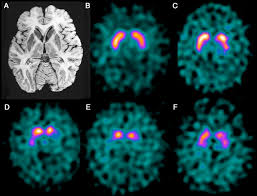
\includegraphics[width=0.5\linewidth]{imagenes/act dopaminergica imagen spect}
	\caption{Actividad dopaminérgica en áreas neuronales específicas afectadas por la enfermedad de Parkinson.}
	\label{fig:act-dopaminergica-imagen-spect}
\end{figure}


Entre ellas destacan el Parkinson (EP), el Alzheimer (EA) y la esclerosis lateral amiotrófica (ELA),
basadas principalmente en la perdida progresiva de células en áreas neuronales específicas. La
EP afecta a las neuronas dopaminérgicas en la sustancia negra, reduciendo los niveles de
dopamina, y a los ganglios basales y llevando a la disfunción del sistema dopaminérgico
cerebral. Esto deriva en la aparición del deterioro cognitivo y problemas de coordinación y
movimiento entre otros. En el caso de la EA, ciertas regiones del cerebro presentan una
disminución de las neuronas colinérgicas, produciendo perdidas en la capacidad de
comunicación y alteraciones en la memoria. En otros casos como la ELA o la enfermedad de
Huntington también deriva en una progresiva parálisis muscular en el primer caso y
movimientos involuntarios en el segundo. \cite{jordan2003avances}\\

Para llegar a entender los efectos producidos por estas enfermedades, hay que poner el foco
en los neurotransmisores afectados por las mismas. EL estudio y análisis de estas variables
permite encontrar un tratamiento que ralentice el avance hacia el declive cognitivo. Por
ejemplo, en el caso del Alzheimer se han desarrollado fármacos que potencian la síntesis de la
acetilcolina, y también inhiben su catabolismo y activan sus receptores. Para el Parkinson, la
levodopa es el tratamiento más eficaz para incrementar la síntesis de la levodopa y para
activar sus receptores. Aún así, tras años de investigación en este ámbito, ningún fármaco ni
tratamiento ha llegado a detener la progresión de estas enfermedades.\\


\subsection{Enfermedad de Parkinson (EP)}

La EP afecta al 1\% de la población mayor de 50 años y tiene una duración estimada de entre 10
y 20 años, afectando de forma progresiva a los pacientes hasta llegar a la invalidez completa. Este trastorno tiene diversas causas:
\begin{itemize}
	\item Alteraciones metabólicas y farmacológicas que afectan a la neurotransmisión de dopamina de los ganglios basales y a las neuronas dopaminérgicas de la sustancia negra.
	\item Pérdida de neuronas estriadas.
	\item Formación de inclusiones celulares llamadas cuerpos de Lewy.
\end{itemize}

\begin{figure}[h]
\centering
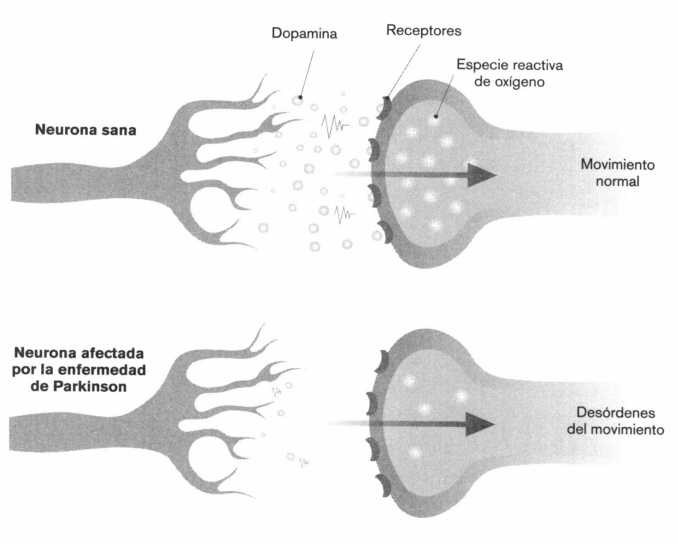
\includegraphics[width=0.5\textwidth]{imagenes/Reducción de transmición dopaminérgica}
\caption{Reducción de la transmisión dopaminérgica de las neuronas afectadas por el Parkinson.}
\label{fig:scan reducción dopamina}
\end{figure}
Entre las principales consecuencias de lo anterior, los pacientes presentas síntomas motores como temblor, rigidez y lentitud de movimientos, pero también no motores como apatía, deterioro cognitivo y síntomas autonómicos. Todo esto afecta drásticamente en la vida de los pacientes. En el caso del Parkinson idiopático (75\% de casos), se distinguen varias fases en función de los indicios detectados: \cite{Elparkin42:online}

\begin{itemize}
	\item Fase inicial con síntomas leves y unilaterales que puede mostrar temblor en
	extremidades superiores entre otros.
	\item Etapa con alteraciones postulares más evidentes y postura encorvada. Aparecen
	síntomas bilaterales.
	\item Se desarrolla incapacidad moderada y alteraciones más pronunciadas, con una dificultad
	de movimiento más resaltado.
	\item Llegando a una fase avanzada de la enfermedad, el individuo requiere asistencia para
	realizar las actividades del día a día debido a la evolución de la incapacidad debida en parte a la
	bradicinesia.
	\item En la última etapa se llega a la incapacidad completa de movimiento.
\end{itemize}

En resumen, a medida que avanza la enfermedad , los problemas motores se generalizan y afectan a ambos lados del cuerpo, mientras la capacidad de procesamiento se deteriora. Todo esto incluye tanto fluctuaciones motoras como no motoras.\cite{martinez2016actualizacion}\\

\subsection{Neurotecnologías}

 La neurociencia y las neurotecnologías han evolucionado mucho desde los descubrimientos de Ramón y Cajal en 1888 hasta los últimos avances en mapas celulares del cerebro humano y en el entendimientos de los circuitos neuronales y la plasticidad cerebral. Sin embargo, hoy en día siguen siendo un gran reto las enfermedades neurológicas, conllevando altos costes y complicaciones. Pero gracias a la combinación de neurociencia con inteligencia artificial y robótica que ofrecen las neurotecnologías modernas, se espera avanzar en la investigación dentro de este ámbito, aunque también habrá que tratar dilemas éticos y morales.\cite{6OFICINA49:online}\\

Existen tres tipos de avances neurotecnológicos: neuroimagen (registro de actividad cerebral), neuromodulación (modificación de señales cerebrales) y neurofeedback (bucle de registro y respuesta de señales). Además, pueden ser tecnologías invasivas, semi-invasivas o no invasivas en función del método de conexión con el sistema nervioso y el riesgo que implican para el paciente.\\

Entra las principales limitaciones debidas a las tecnologías actuales se encuentra: la complejidad de captar la actividad neuronal de forma no invasiva y con alta precisión, y la dificultad de manejar grandes cantidades de datos. Como respuesta, se están intentando desarrollar materiales y técnicas para una mejor resolución y seguridad en el registro de actividad cerebral. Además, gracias al uso de la inteligencia artificial como herramienta para procesar la gran cantidad de información, se puede procesar y entender de manera más eficaz, permitiendo tratamientos más avanzados. Esto permite llevar a cabo tratamientos más efectivos y personalizados para distintas condiciones neurológicas.\\

El principal enfoque de las neurotecnologías es ayudar a personas con discapacidades motoras y sensoriales. Para ello, se están investigando las interfaces cerebro-ordenador que, combinadas con fisioterapia, muestran resultados prometedores para la rehabilitación de extremidades paralizadas. La estimulación de la plasticidad neuronal conseguida debido a los avances en el diseño de neuroprótesis y robots, también facilita la recuperación funcional de los pacientes.  \\

Por otro lado, también se están desarrollando dispositivos que permitan restaurar la audición y la visión, como pueden ser los implantes cocleares, ya utilizados para tratar la sordera, o los implantes de retina, que aun están siendo investigados pero que permitirían recuperar la capacidad visual.\\

Además, hay un campo de investigación centrado en la decodificación cerebral tanto del lenguaje como del pensamiento visual y de los estados emocionales. El objetivo es mejorar la comunicación mediante interfaces cerebro-ordenador de personas con parálisis. Por ejemplo, algunas de las nuevas tecnologías que se están llevando a cabo traducen la actividad cerebral para que pueda ser interpretada por una computadora. También se avanza en reconstruir imágenes visuales observadas y en comprender estados emocionales y niveles de conciencia, útiles tanto para mejorar la calidad del sueño como para tratar trastornos neuropsiquiátricos como la depresión.\\

En cuanto a la realidad virtual, puede llegar a tener un gran potencial en combinación con las interfaces cerebro-ordenador, por ejemplo para trata pacientes tetrapléjicos u para otros fines medico y también en el ámbito de los videojuegos. Además, muchas empresas están realizando importantes inversiones, por lo que a pesar de implicar altos costes se están volviendo cada vez más accesibles. Se espera que en los próximos años estas tecnologías mejoren la capacidad cognitiva y la consciencia, pero también se deberán tratar dilemas legales y éticos, ya que por ejemplo, la privacidad mental y la seguridad de los neurodatos estarán en el punto de mira debido a los riesgos de violaciones de privacidad que pueden venir de la mano de las neurotecnologías y la inteligencia artificial. Por ello, es crucial que haya un consentimiento informado para que los distintos riesgos.\\

En cuanto a los altos costes, estos pueden derivar en diferencias sociales en función del acceso a estas tecnologías. También es muy importante tener en cuenta los efectos adversos a largo plazo que pueden tener además de todos sus beneficios y mejoras en el aprendizaje y la memoria, siendo crucial una regulación ética y legal estricta.\\

Diversos organismos internacionales y nacionales están estableciendo marcos legales que protejan lo conocido como neuroderechos. Las Iniciativas impulsadas por grupos como la UNESCO o la OCDE han hecho resaltar la necesidad de una regulación global, mientras que en Europa aun no existe una legislación especifica para las neurotecnologías. Sin embargo, en diversos países como España o Francia ya han incluido los neuroderechos en sus constituciones, avanzando así en la protección de datos neuronales. También se ha reflejado un compromiso Europeo y Español de la promoción de neuroderechos con las declaraciones de León y Valencia.\\

En España, la regulación de las neurotecnologías está enfrentándose a desafíos importantes:
\begin{itemize}
	\item La Agencia Española del Medicamento y Productos Sanitarios (AEMPS)se encarga de supervisar evaluaciones clínicas estrictas, intentando asegurar la seguridad y eficacia de estas tecnologías.
	\item La Red Española de Agencias de Evaluación de Tecnologías Sanitarias (RedETS) gestiona la inclusión de estas tecnologías en la cartera de servicios del Sistema Nacional de Salud.
	\item El Reglamento (UE) 2022/2346 regula las neurotecnologías no invasivas fuera del ámbito clínico, que pide evaluaciones exhaustivas de riesgos y efectos.
\end{itemize}

Desde 2013, se han invertido significativas sumas en proyectos globales de investigación cerebral como BRAIN en EE.UU. y el Proyecto Cerebro Humano en Europa, buscando avanzar en neurotecnologías para comprender mejor la actividad neuronal y su impacto en la cognición. Se enfatiza la creación de infraestructuras científicas y plataformas digitales para facilitar el acceso a datos y herramientas de modelización. La comunidad científica aboga por aumentar la financiación y la colaboración interdisciplinaria para acelerar la aplicación clínica y social de estos avances, destacando la importancia de una regulación ética que promueva la innovación responsable.\\


\subsection{Modelos Predictivos}
No cabe duda que la creación y avance de modelos predictivos para predecir la evolución de la enfermedad de Parkinson, incluido el declive cognitivo, reviste una importancia crucial, permitiendo avanzar en diagnósticos más personalizados y precisos. Actualmente existen diversos modelos predictivos basados en datos clínicos, genéticos y de imagenología, como lo que se han utilizado en el presente estudio, que han demostrado cierto grado de precisión en la predicción de la progresión de la enfermedad.\\

Estos modelos emplean técnicas estadísticas y de aprendizaje automático para analizar grandes conjuntos de datos y extraer patrones y tendencias relevantes. Sin embargo, aún hay desafíos importantes por superar, como la heterogeneidad de la enfermedad y la necesidad de datos longitudinales y multimodales para una predicción más precisa. \cite{Predicti52:online}\\

En este contexto, la inteligencia artificial (IA) emerge como una herramienta prometedora que permitirá avanzar en el diseño de modelos predictivos más precisos y personalizados para la enfermedad de Parkinson. Los algoritmos de IA, como las redes redes de muestreo como puede ser Leaspy,
tienen el potencial de manejar datos complejos y heterogéneos de manera más efectiva, identificando
correlaciones sutiles y no lineales que pueden pasar desapercibidas para los enfoques tradicionales.\\

En resumen, avanzar en el diseño de modelos predictivos para la enfermedad de Parkinson, incluido el
declive cognitivo, es fundamental para mejorar la atención médica y la calidad de vida de los pacientes.
La aplicación de la inteligencia artificial abre nuevas posibilidades para lograr predicciones más precisas
y personalizadas, allanando el camino hacia una atención médica más efectiva y centrada en el paciente.\\

\subsection{Impacto socioeconómico}
La enfermedad de Parkinson tiene un impacto significativo en el ámbito socioeconómico, afectando a los pacientes, a sus familias y a la sociedad en general. Además, cada vez tiene más relevancia debido al constante cambio que sufre el contexto demográfico, caracterizado por el envejecimiento general de la población debido al aumento de la esperanza de vida y a la disminución de la natalidad. Esto tiene crucial importancia ya que el Parkinson afecta principalmente a personas de avanzada edad, viendo como dicho grupo está aumentando considerablemente. Esta tendencia tiene importantes implicaciones para la salud pública y el sistema de atención médica, ya que el envejecimiento de la población se asocia con un mayor riesgo de enfermedades crónicas, discapacidades y necesidades de atención a largo plazo. \cite{GARCIARAMOS2016401}\\

En este contexto, el impacto socioeconómico del Parkinson adquiere una mayor relevancia, ya que afecta a un segmento cada vez mayor de la población. El tratamiento y manejo de esta enfermedad pueden generar una carga económica significativa para los pacientes y sus familias, especialmente en un entorno demográfico en el que un mayor porcentaje de la población está en edad de jubilación y puede tener recursos financieros limitados.\\

La enfermedad de Parkinson en España genera unos costes importantes, que llegan a alcanzar los 17.000 euros anuales por paciente. Los costes directos, principalmente los tratamientos médicos, llegan a una media de 8.640 euros cada seis meses, de los que 1.456 euros se destinan a medicamentos dopaminérgicos \cite{GARCIARAMOS2016401}. Los costes indirectos, como la pérdida de productividad por jubilación anticipada, aumentan hasta los 6.691 euros por persona en tres meses. Las terapias avanzadas, como la estimulación cerebral profunda (DBS), tienen un coste a cinco años de 88.104 euros, mientras que la infusión subcutánea continua de apomorfina (ICAS) cuesta 141.393 euros y la infusión intraduodenal de levodopa (ICLI) 233.986 euros. Anualmente, estos tratamientos suponen unos costes de 17.603 euros para la DBS, 28.279 euros para la ICAS y 46.796 euros para la ICLI.\\

Además, los casos de Parkinson han sufrido un fuerte aumento, tal y como se ve en la gráfica de la figura \ref{fig:graf_Park_esp} que representa la evolución del Parkinson en España entre el año 2011 y 2022. \cite{RegParkEsp}\\


\begin{figure}[t]
	\centering
	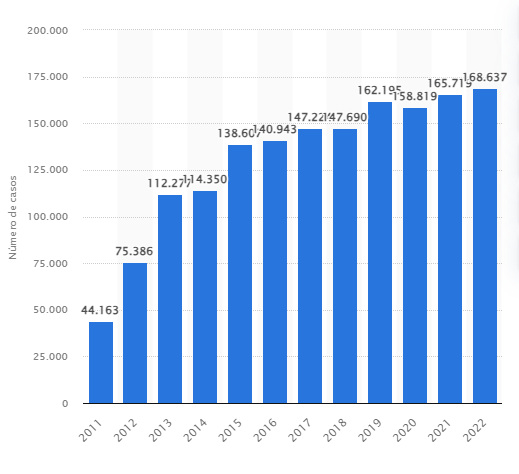
\includegraphics[width=0.7\textwidth]{imagenes/registro_Parkinson}
	\caption{Cifras de casos de Parkinson registrados en España entre los años 2011 y 2022.}
	\label{fig:graf_Park_esp}
\end{figure}

Además, los síntomas motores y no motores del Parkinson pueden afectar la calidad de vida de los pacientes, limitando su participación en actividades sociales y recreativas y generando sentimientos de aislamiento y depresión. Esto puede tener un impacto negativo en el bienestar emocional y social de los pacientes, así como en su capacidad para llevar una vida plena y satisfactoria.\\


\section{Objetivos}
Actualmente, para poder mejorar los tratamientos para las enfermedades neurodegenerativas es necesario poder predecir su aparición y evolución lo antes posible. Se parte de la premisa fundamental de que la detección precoz y el seguimiento preciso de la progresión de la enfermedad son esenciales para mejorar la calidad de vida y ralentizar su avance. Por ello, el objetivo principal de este trabajo es utilizar el entorno de programación para Python llamado \textit{Leaspy}, para predecir la aparición de declive cognitivo en pacientes con enfermedad de Parkinson.\\

\textit{Leaspy} es un paquete de software que facilita el análisis de datos longitudinales como pueden ser los recopilados en la base de datos utilizada, compuesta por observaciones repetidas de un grupo de 423 pacientes a lo largo del tiempo. Esta está formada por datos médicos recopilados de distintas visitas de un grupo de pacientes. \\

Con el programa desarrollado se pretende medir si las predicciones obtenidas utilizando esta herramienta son mas precisas que los resultados obtenidos por otros algoritmos, como el 'Robust Paramétric Disease Progresssion Modeling' (RPDPM). Con esta meta, se calculan diversos parámetros que miden la precisión de los Modelos de Progresión de la Enfermedad (DPMs, por sus siglas en inglés), estimados previamente gracias a funciones características de \textit{Leaspy}. Las prestaciones indican por un lado, la precisión de la trayectoria estimada de la enfermedad en los sujetos, y por otro lado, la exactitud del pronóstico de aparición del declive cognitivo en los pacientes. Todo esto queda reflejado en los parámetros de error absoluto medio (MAE), Área Bajo la Curva (AUC), correlación de de la edad de conversión, correlación de la reserva cognitiva, etc. \\

Además de comparar \textit{Leaspy} con otros métodos de predicción, también se busca comparar los modelos estimados caracterizados por estimar la evolución de la enfermedad en los sujetos a partir de distintos conjuntos de biomarcadores. Por lo que otro de los objetivos de este estudio es encontrar el conjunto de biomarcadores con el que se obtenga una predicción lo más precisa posible de la trayectoria de la enfermedad en los individuos y de la aparición del deterioro cognitivo leve (MCI).\\

En conjunto, este estudio aspira a contribuir significativamente al avance del conocimiento en la estimación de modelos de progresión de la enfermedad de Parkinson, así como a comprender más a fondo el progreso de este tipo de enfermedades.


\section{Estructura del documento}

A continuación y para facilitar la lectura del documento, se detalla el contenido de cada capítulo.

\begin{itemize}
\item En el capítulo 1 se realiza una introducción.
\item En el capítulo 2 se hace un repaso de distintos recursos cruciales para esta investigación.
\item En el capítulo 3 se nombran las distintas herramientas y materiales utilizados en este trabajo.
\item En el capítulo 4 se explica el algoritmo desarrollado. 
\item En el capítulo 5 se muestran los resultados obtenidos y se discuten.
\item En el capítulo 6 se concluye el trabajo y se reflejan los pasos futuros.
\end{itemize}

  
%partes finales del trabajo: conclusiones, bibliografia y anexos
  
\chapter{Estado de la técnica}

\section{Neurodegeneración: Alzheimer, Parkinson y ELA}

Este libro, plantea el objetivo de transmitir de manera sencilla y clara conceptos básicos de la neurodegeneración y de las principales enfermedades neurodegenerativas, intentado simplificar algo tan complejo como el cerebro humano. \cite{Neurodeg64:online}

\subsection{Definición y concepto}

Inicialmente, se establece la definición básica de envejecimiento como principal factor de riesgo para el proceso degenerativo. A continuación, se trata superficialmente los mecanismos importantes tanto en el envejecimiento como en la degeneración, y se expone la definición del mismo en lo relacionado con el cerebro.\\

La definición del envejecimiento se centra en la pérdida de vitalidad y el aumento progresivo de la vulnerabilidad y la fragilidad.  Este proceso biológico universal, progresivo, determinado-regulado, supresor heterogéneo e irreversible, conlleva una progresiva e irreversible pérdida de la integridad fisiológica.\\

En la sociedad actual, la esperanza de vida tiende a un incremento progresivo. En los países desarrollados está en aumento, tanto la Edad Media de la población como el porcentaje de personas dentro del rango entre 85 y 100 años. Esto pone en el punto de mira la búsqueda del retraso de la aparición de enfermedades asociadas al envejecimiento.\\

Gracias a varias investigaciones, se ha descubierto que las dietas calóricas son un importante factor de disminución de las expectativas de vida. Mediante mecanismos de reprogramación que restringen la cantidad de calorías en la alimentación, se consiguió incrementar la longevidad en numerosas especies y mejorar diversas actividades metabólicas. \\

Por otra parte, ganó importancia la identificación de genes encargados de modular la longevidad. En algunos modelos animales se identificaron elementos modificadores asociados al aumento de las expectativas de vida, como por ejemplo:
\begin{itemize}
	\item Disminución del factor de crecimiento insulina-like (IGF.1)
	\item Disminución de la proteína mTOR
	\item Aumento de la actividad de las siete sirtuinas conocidas, sobre todo de la sirtuina 1 (SIRT1) mediante la ingesta de resveratrol
\end{itemize}

Otro factor fundamental en esta línea de investigación es la epigenética. Actualmente se la define como el estudio de cambios heredables en la función genética que se producen sin ningún cambio en la secuencia del ADN. Es una ciencia que estudia la forma, como los factores ambientales y de estilo de vida que influyen en la expresión final de ciertos genes. Por esto mismo, el 
epigenoma cambia durante toda la vida en función de estas variables, siendo muy flexible y conllevando grandes implicaciones en el campo de la salud.\\

Muchas de las enfermedades debidas al envejecimiento, como algunos tipos de demencia, presentan un componente epigenético. Al envejecer, se pierden grupos metilos, las neuronas disminuyen o dejan de producir determinados neurotransmisores.\\

La posibilidad de lograr un rejuvenecimiento con los cambios epigenéticos, lleva a hablar de la reprogramación celular. Esto se el método para la modificación del epigenoma.	Mediante la combinación de cuatro genes, llamados los factores de Yamanaka pudo conseguirse la detención o reversión del envejecimiento. Esto fue descubierto por Shanya Yamanaka en el 2006, al convertir una célula adulta en una célula madre pluripotente. Para evitar que haya más probabilidad de desarrollar células tumorales, se llegó a la conclusión de no permitir la finalización del proceso de transformación.\\

Los factores ambientales modulan mecanismos epigenéticos que a su vez, modulan la capacidad funcional de las células madre.  Un decline de la funcionalidad de estas, lleva a la perdida de homeostasis. Recientemente se demostró la posibilidad de obtener células funcionalmente completas a partir de células senescentes. Esto era algo inimaginable hace no tanto en la reprogramación celular, por lo que esto muestra una evidencia adicional a la reversión del envejecimiento celular. Esto podría concluir en mejoras terapéuticas para personas con progeria.\\

Por otro lado, Se sugiere la existencia de un reloj metabólico que controla el envejecimiento. Este Se basa en 9 sellos distintivos del envejecimiento, los cuales los podemos clasificar en 3 categorías. En La primera, nos encontramos con las principales causas del daño molecular, Como la inestabilidad genómica Basada en la rotura del equilibrio entre los daños y la capacidad de reparación; Alteraciones epigenéticas que cambian la estructura del ADN; pérdida de proteostasis Y desgaste del telómero. La segunda categoría están los componentes beneficiosos a niveles bajos y dañinos a niveles altos. Entre ellos se encuentran la disfunción mitocondrial, la senescencia celular, o la detección desregulada de nutrientes. Por último, Se encuentran los elementos con los que desaparece la capacidad de autorregulación, Como el cansancio de células madre y las alteraciones en la comunicación intercelular.\\

La neurodegeneración consiste en el deterioro de células y tejidos, haciendo que estos pierdan de forma gradual la capacidad para realizar sus funciones. Por otra parte, esta la regeneración, proceso donde se restablecen células, tejidos y órganos. En cambio, las neuronas son células postmitóticas no tienen la habilidad de dividirse ni remplazarse, por lo que envejecen por la acumulación de daños con el paso del tiempo. Esto lleva a una pérdida de neuronas que afecta sobre todo al hipocampo y a los cingulados anterior y posterior, zonas especialmente afectadas en las enfermedades neurodegenerativas. También supone una pérdida de dendritas y sinapsis. 
Hay varios mecanismos encargados de inducir la neurodegeneración. Entre ellos encontramos factores diversos como pueden ser genéticos y ambientales, las dinámicas anormales de las proteínas o el daño oxidativo.   Todo esto junto con otros sistemas llevan a la muerte celular.\\

Intentando aclarar el mecanismo de degeneración de las células, algunos científicos llegaron a la conclusión de que la agregación de proteínas alteradas o deficientemente plegadas eran una de las principales causas de la muerte neuronal. Las distintas enfermedades neurodegenerativas tienen esta característica en común. Mediante distintos estudios, se consiguieron identificar ciertas alteraciones de proteínas correspondientes a diferentes enfermedades. Como, por ejemplo, el Alzheimer se asocia a la proteína B amiloide y el Parkinson a los depósitos de alfa-sinucleína.  Aún así, siguen abiertas ciertas preguntas, como el por qué de que algunas proteínas se plieguen de forma anormal y por qué algunas son más propensas a la agregación que otras.
Otro concepto muy importante y bastante reciente es la resiliencia. Esta consiste en la capacidad de los individuos a ajustarse a situaciones adversas o, en el ámbito de la física, es la capacidad de ciertos materiales para recuperarse de ciertas cargas. Los factores determinantes de la resiliencia pueden ser determinantes para las investigaciones de la neurodegeneración.

\subsection{Bases moleculares y celulares de la degeneración}

El conocimiento de las bases moleculares y celulares de la neurodegeneración son esenciales para desarrollar nuevos métodos diagnósticos así como nuevas terapias. En el libro se aborda la compleja interacción entre los diferentes procesos biológicos y fisiológicos que pueden influir en la patogénesis de diferentes enfermedades. Se ha hecho un enorme esfuerzo en estudiar los mecanismos que regulan la muerte celular, ya que esto permitirá avanzar en nuevas intervenciones terapéuticas que detengan o enlentezcan el proceso neurodegenerativo.\\

Se describen tres tipos de muerte celular: la apoptosis o “muerte celular programada”, la necrosis que se produce como consecuencia de la acción de toxinas, generando una caída de ATP y la autofagia. Este último, es un mecanismo empleado por las células eucariotas para degradar sus componentes con vistas a la renovación y recambio de estos. Se concluye que en la neurodegeneración la autofagia está descontrolada. Después de analizar este mecanismo en las principales enfermedades degenerativas, se concluye que se encuentran involucrados de una manera directa defectos en su funcionamiento.\\

Otro de los procesos objeto de estudio es la oxidación y el estrés oxidativo. Esto es debido a nuestra naturaleza como seres vivos que consumen oxígeno y que están expuestos de manera permanente a subproductos tóxicos conocidos genéricamente como  “radicales libres de oxígeno” y “radicales libres de hidrógeno”. Uno de los radicales libre de mayor interés en medicina es el óxido nítrico, se estima que tiene un papel protagonista indirecto en la neurodegeneración a través de un derivado denominado “peroxinitrito”. Los resultados de diferentes estudios demuestran que la generación de prooxidantes es un factor que influye en la velocidad de envejecimiento, el cual está relacionado directamente con el daño mitocondrial.\\

Por tanto, en el origen de las enfermedades neurodegenerativas se encuentran involucrada la elevada producción de especies reactivas de oxígeno (ROS) y especies reactivas de nitrógeno (RNS) asociadas a un mal funcionamiento de la mitocondria neuronal. El daño en el ADN, como consecuencia del estrés oxidativo, genera desarrollo de mutaciones en el mismo. En definitiva, se genera una relación multidireccional entre estrés oxidativo, mal funcionamiento mitocondrial, incremento de apoptosis y disminución de la autofagia, cuyo resultado es el desarrollo de la neurodegeneración.\\

Un último elemento a analizar es la neuroinflamación como respuesta inflamatoria del sistema nervioso central a cualquier tipo de agresión o lesión sobre este. En este punto es relevante las funciones que tiene la glía, células que desempeñan un papel esencial de soporte a las neuronas y a ala fisiología del sistema nervioso. Aunque el proceso inflamatorio es un mecanismo de defensa del organismo contra la infección, la pérdida de su regulación hace que contribuya a una condición patológica, pues mantiene un proceso de destrucción celular progresivo. Esto nos lleva a que las respuestas inflamatorias se mantienen activadas durante el estado de estrés oxidativo, lo que lleva a las neuronas a un círculo vicioso de muerte y destrucción.	

\subsection{Enfermedades neurodegenerativas}

Las enfermedades degenerativas tienen cada vez mayor protagonismo en nuestra sociedad debido al envejecimiento de la población. Se definen como aquellas patologías heredadas o adquiridas, en las que se produce una disfunción progresiva del sistema nervioso central. Existen más de 600 enfermedades neurodegenerativas, pero destacan la enfermedad de Alzheimer (EA), la enfermedad de Parkinson (EP), la enfermedad de Huntington (EH) y la esclerosis lateral amiotrófica (ELA).

\subsubsection{Enfermedad de Alzheimer}

La EA es actualmente un problema de primer orden y una prioridad para los sistemas de salud. Hay varios estudios sobre su prevalencia, el estudio Delphi prevé que en el 2040 habrá más de 80 millones de personas afectadas por la enfermedad, existiendo unanimidad en que la prevalencia se dobla cada cinco años. Siendo una de las principales causas de muerte no se puede prevenir, curar ni siquiera ralentizar su avance.
La edad es el principal factor de riesgo para su desarrollo, y presenta mayor incidencia en el género femenino en edades avanzadas, también un abaja escolarización aumenta el riesgo. Existen multitud de estudios sobre los diferentes factores de riesgo, una relación compleja difícil de interpretar debido a la alta variabilidad. La mayoría de los casos se considera que no tienen origen genético. Sin embargo, existen pruebas de factores genéticos que puedan conllevar una mayor predisposición a padecer la enfermedad, confirmándose el genotipo apolipoproteçina E (ApoE) como factor de riesgo en múltiples estudios.
En la corteza cerebral, la sustancia blanca contiene los axones (responsables de las conexiones entre neuronas). La pérdida de sinapsis podría constituir la vía final común de la patología, ya que su número disminuye con la evolución de la enfermedad.\\

Existe la necesidad de definir el estado entre normalidad y demencia y para ello han surgido en los últimos años diferentes criterios, cobrando especial relevancia en el mundo científico el término “deterioro cognitivo leve”. Los pacientes se quejan básicamente de pérdida de memoria, pero pueden manifestar otras dificultades. Las técnicas de neuroimagen son de indudable interés clínico, de forma complementaria a las manifestaciones clínicas. El objetivo es identificar a aquellos pacientes con mayor riesgo de desarrollar una demencia, e instalar un acercamiento terapéutico de manera temprana.
La demencia es un proceso progresivo. Al déficit de memoria se van añadiendo dificultades del lenguaje, la desorientación y la desorganización de las actividades cotidianas. Entre otras manifestaciones clínicas se encuentra la apraxia y la agnosia y la afasia en sus diferentes manifestaciones. Los síntomas psicológicos y conductuales afectan a los pacientes con demencia, con una prevalencia del 90\%, entre los que cabe destacar la apatía, la agresividad, así como las alucinaciones y la alteración del ciclo vigilia-sueño. Es relevante ubicar al paciente en el estadio evolutivo para programar adecuadamente su tratamiento.\\

El diagnóstico sigue siendo fundamentalmente clínico. Aunque en la ayuda al diagnóstico se empiezan a incorporar diversos biomarcadores, así como técnicas de imagen como la resonancia nuclear magnética, la tomografía por emisión de fotón único (SPECT) o la tomografía por emisión de positrones con fluordeoxiglucosa (PET-FDG). Esta última ha demostrado su utilidad para distinguir pacientes con EA de otras demencias. Otras técnicas de imagen pueden ser útiles para el diagnóstico precoz y el seguimiento de la enfermedad.\\

La intervención terapéutica debe contemplar tratamiento farmacéutico, intervención no farmacológica,  y la actuación sobre familiares/cuidadores. El tratamiento farmacológico se centra en paliar la degeneración neuronal, potenciar la actividad de las neuronas no afectadas y aliviar los síntomas de la enfermedad. El tratamiento se centra en dos grupos de fármacos: los inhibidores de acetilcolinesterasa (IACE) y los antagonistas de los receptores N-Metil-D-Aspartano tipo memantina. Una línea abierta de investigación es la búsqueda de tratamientos que sean modificadores de la historia natural de la enfermedad, destacando el dirigido contra la proteína beta amiloide o la inmunoterapia activa. En lo que respecta a las intervenciones no farmacológicas, cabe destacar: programas de orientación a la realidad, terapia de reminiscencia, terapia de validación, estimulación cognitiva y estimulación magnética. Entre las medidas aplicadas al cuidador, señalar las orientadas a los programas de información y formación, los equipos de soporte domiciliario y las unidades de apoyo sociosanitario.\\

En términos de coste económico, se considera que las demencias son la tercera causa más costosa, tras el cáncer y las enfermedades cardiovasculares. En más del 80\% de los casos, el cuidado lo realiza la familia. El diagnóstico precoz y el empleo de alternativas no farmacológicas podrían reducir el coste total de las demencias.		

\subsubsection{Enfermedad de Parkinson (EP)}

Es un trastorno neurodegenerativo crónico de curso progresivo y evolución prolongada, caracterizado por la pérdida de neuronas dopaminérgicas. Se trata de la segunda enfermedad neurodegenerativa más frecuente en mayores de 65 años, tras la enfermedad del Alzheimer y afecta entre el uno y el dos por ciento de la población. En la mayoría de los casos es de tipo esporádico y de causa desconocida.\\

Las manifestaciones iniciales suelen pasar desapercibidas. Un síntoma común suele ser el temblor en reposo y de tipo asimétrico que afecta a la mano, aunque pueden aparecer otros síntomas iniciales. Existen una serie de síntomas no motores cuya presencia puede poner sobre aviso: trastornos en el olfato, alteraciones en la fase REM de sueño y el estreñimiento. El diagnóstico precoz a través de biomarcadores es primordial, desde técnicas de neuroimagen hasta marcadores genéticos, moleculares y tisulares. Las principales manifestaciones clínicas son: Bradicinesia. Temblor, Rigidez e inestabilidad postural. A estos se les pueden unir otros síntomas motores de manera variable: Disfagia, Síndrome de piernas inquietas y alteraciones del lenguaje. Entra las manifestaciones no motoras se encuentran: depresión, ansiedad, apatía,  en algunos casos problemas de vejiga o de estreñimiento, excesiva producción de saliva o inadecuada deglución, así como problemas en la piel. Un diagnóstico temprano puede ser difícil por falta de biomarcadores con suficiente nivel de sensibilidad y especificidad. El infradiagnóstico se sitúa en un 24 \% y es frecuente un diagnóstico erróneo. Pueden ser de ayuda pruebas de neuroimagen funcional.\\

No hay cura para la EP, pero distintos medicamentos pueden proporcionar un significativo alivio en fases iniciales y debe continuarse durante casi toda la vida del paciente. La levopoda es el tratamiento sintomático más eficaz, permitiendo a los pacientes alargar el período de tiempo en el que poder llevar una vida relativamente normal. Otros fármacos, aunque menos eficaces en controlar la rigidez y la bradicinesia son la bromocriptina y la pergolida. La Selegilina se está utilizando también para la EP, pudiendo realzar y prolongar la respuesta de la levopoda. También se está experimentando con injertos naturales o el trasplante de células nerviosas, así como con el uso de células genéticamente producidas.\\

También es preciso un abordaje integral y multidisciplinar de la enfermedad, con el objetivo de mejorar o mantener la calidad de vida del paciente y sus cuidadores. Desde el ejercicio físico, la fisioterapia, las terapias ocupacionales, entre otras. Todas ellas suman para retrasar el deterioro.		

\subsubsection{Esclerosis lateral amiotrófica (ELA)}

La ELA es la enfermedad de la neurona motora más frecuente en adultos y se basa en la degeneración combinada de las motoneuronas superiores e inferiores. La consecuencia es una debilidad muscular que avanza hasta la parálisis. Su incidencia está entre 0,4-1,8/100000hab y año. Además, es más frecuente en hombres y la supervivencia media es de 3 años.\\

Los primeros síntomas suelen ser espasmos musculares y debilidad en un miembro o dificultad para hablar, afectando posteriormente a los músculos necesarios para moverse, hablar o comer. Sólo un 10 \% puede desarrollar deterioro cognitivo. Por otra parte, es difícil de diagnosticar de manera temprana y un método de ayuda es el electromiograma. Actualmente no existe ningún tratamiento eficaz, el único que ha demostrado prolongar la supervivencia es el riluzol. Todos los esfuerzos deben ir encaminados a conseguir mejor calidad de vida de pacientes y familiares. El avance de la enfermedad plantea decisiones de gran dificultad ética que deben ser compartidos con los pacientes y su familia.


\subsubsection{Enfermedad de Huntington}
Se trata de un trastorno neurodegenerativo con carácter hereditario autosómico dominante. Presenta tres manifestaciones clínicas principales: movimientos involuntarios bruscos, alteraciones de la personalidad y deterioro mental. Con una prevalencia de 5-10 casos por 100.000 habitantes, afecta igual a hombres y mujeres.\\

El diagnóstico se basa en las características clínicas y los antecedentes familiares confirmados por análisis genético del ADN. No existe tratamiento que cure o ralentice el avance, por lo que está orientado a mejorar la calidad de vida a través del tratamiento sintomático. Las vías de investigación incluyen la interferencia en RNA que operaría en el inicio del proceso. La asistencia sociosanitaria es clave en este trastorno.

\subsection{Intervención terapéutica}

Los condicionantes del estilo de vida tienen un profundo impacto en nuestro cerebro. Son tres los elementos principales a tener en consideración para prevenir los procesos neurodegenerativos: ejercicio físico, nutrición y actividad intelectual.\\

Hoy podemos establecer que la actividad física es uno de los mejores neuroprotectores existentes, demostrando mejores parámetros cognitivos asociados a la edad. Se sabe que el ejercicio físico influye en la capacidad de generar nuevas neuronas y nuevas conexiones, favoreciendo un incremento de las neurotrofinas que promueven mayores conexiones entre áreas del cerebro, además de su acción antiinflamatoria. Existe diferentes tipos de ejercicio (aeróbico, anaeróbico y de resistencia) que deben tenerse en cuenta en función de estado del paciente, en base a un análisis individualizado. Como conclusión, el ejercicio físico mejora la función cognitiva en adultos mayores de 50 años, debiendo incluir una duración mínima de 45 minutos en intensidad de moderada a vigorosa.\\

Por otro lado, hay que señalar que a actividad intelectual está directamente relacionada con el concepto de reserva cognitiva, como la capacidad del cerebro para tolerar diversas patologías. Existen varios factores asociados al desarrollo de nuestra capacidad cognitiva: volumen cerebral, educación y complejidad laboral, bilingüismo y actividad mental y estimulación cognitiva. Sin embargo, los estudios sobre estos aspectos están sujetos a limitaciones metodológicas, siendo necesario el desarrollo de estudios multidisciplinares que avancen en la evidencia científica.\\

Por último, no podemos dejar de hablar de la importancia del consumo de alimentos saludables como un gran aliado en la prevención de enfermedades neurodegenerativas. Diferentes estudios señalan que modificaciones nutricionales pueden tener un fuerte impacto en la salud. Más allá del papel que puedan desempeñar ciertos nutrientes, lo más relevante es la adopción de la dieta mediterránea como estilo de vida saludable. Los componentes de esta pueden actuar como factores de neuroprotección, como restricción calórica o como antioxidantes naturales. Hay pocos estudios que relacionen patrones dietéticos y enfermedades neurodegenerativas, centrándose más en alimentos aislados. Quedan preguntas por contestar, pero parece claro que la intervención deber realizarse incluso antes de la edad adulta para conseguir la mayor acción preventiva.\\




\section{Clinical variables and biomarkers in prediction of cognitive impairment in patients with newly diagnosed Parkinson’s disease: a cohort study}


\subsection{Introducción}

La enfermedad de Parkinson provoca un deterioro cognitivo consistente en la disminución de capacidades como memoria, atención o razonamiento. En etapas mas avanzadas, aparece la demencia que incapacita a los pacientes en su vida diaria. El desarrollo de métodos de predicción basados en el declive cognitivo leve en etapas tempranas, permitiría avanzar en la detección de la enfermedad. \\


La deficiencia en dopamina ha sido identificada como un indicador eficiente relacionado con el deterioro cognitivo. Además se han sugerido otros factores como la edad o el género. En este estudio se valora la inclusión de los niveles de líquido cefalorraquídeo (CSF-cerebrospinal fluid) e imágenes de transporte de dopamina (DAT) para predecir el declive cognitivo en un periodo de 2 años \cite{schrag2017clinical}.

\subsection{Métodos}
En este estudio se trabajó con la información de pacientes de la Parkinson’s Progression Marker Initiative (PPMI), en el cual se hace una evaluación clínica de dos grupos. Por una parte, se encuentran los pacientes a los que se les ha detectado la enfermedad de Parkinson y, por otra, un grupo de control formado por individuos sanos. Con las personas seleccionadas se llevó a cabo un seguimiento de dos años (Julio, 2010 - May, 2013). El grupo de control se seleccionó en base a su similitud con el de los pacientes, para poder realizar un análisis comparativo entre ambos colectivos. Para ello se utilizó un método de exclusión con algunos requisitos como: trastornos neurológicos clínicamente significativos o tener algún familiar de primer grado con Parkinson.\\

Los factores evaluados en este estudio fueron: 
\begin{itemize}
	\item Funciones motoras y no-motoras.
	\item Examen del líquido cefalorraquídeo (CSF).
	\item Imagen de emisión de fotón único con tomografía computarizada (SPECT) de ioflupano marcado con yodo-123 en DATSCAN.
\end{itemize}

Los cuales se analizaron a través de ciertas capacidades: memoria (HVLT-R), función visuoespacial (Benton Judgment of Line Orientation 15-item (split-half)), velocidad de proceso y atención, función ejecutiva y memoria de trabajo, y la fluencia. Se empleó cómo método de validación global de las citadas habilidades la escala MoCA (Montreal Cognitive Assesment). En función de los resultados de estas pruebas que se realizan durante un seguimiento de 2 años, los pacientes son clasificados en tres grupos:
\begin{enumerate}
	\item Cognición normal.
	
	No presenta ningún cambio en las habilidades cognitivas.
	
	\item Deterioro cognitivo medio.
	
	Aparecen ciertas puntuaciones en mínimo dos de los tests cognitivos  realizados, pero no llega a influir en las capacidades funcionales.
	
	\item Demencia.	
	
	Se detecta un deterioro funcional debido al decline cognitivo que afecta ala vida diaria del paciente.
\end{enumerate}

Además de las variables clínicas que se incluye en el estudio por estar relacionadas con el deterioro cognitivo(edad, género, años de educación, duración de la enfermedad, sentido del olfato, trastorno dela conducta del sueño por movimientos oculares rápidos(RBD), depresión, severidad de la enfermedad de Parkinson, ...), también se incluyen algunos biomarcadores ya nombrados anteriormente: 
\begin{itemize}
	\item Datos de imágenes DAT.
	\item Estado del APOE$\epsilon$4.
	\item Valoración del CSF (Líquido cefalorraquídeo).
\end{itemize}

En el proceso analítico de los datos seleccionados se identifican 5 pasos en su ejecución:

\begin{description}
	
	\item {\textbf{Paso 1}} Recopilación y evaluación de datos.
	
	Se recogieron datos en dos momentos clave, en la linea de base, donde se realizo el cuestionario MoCA y se tomaron imagen de DAT; y a los dos años de seguimiento. La diferencia entre estas dos medidas se guardo como el cambio en el puntaje MoCA. \cite{bland1995comparing}
	
	\item {\textbf{Paso 2}} Búsqueda de datos faltantes.
	
	Se utilizaron técnicas de imputación y análisis de regresión.
	
	\item{\textbf{Paso 3}} Pruebas de comparación de grupos.
	
	En función de la naturaleza de las variable se realizaron: pruebas chi-cuadrado	para variables categóricas, pruebas t para variables con distribución normal y pruebas de Mann-Whitney para las no paramétricas.
	
	
	\item {\textbf{Paso 4}} Análisis de regresión.
	
	En función del tipo de la variable de respuesta y del modelo se llevaron a cabo:
	
	\begin{enumerate}
		\item Análisis de regresión lineal. (variable continua)
	
		Para observar el cambio en el puntaje MoCA en función de variables independientes, fueron tanto univariadas como multivariadas. 
	
		\item Análisis de regresión logística. (variable categórica o binaria) \cite{bursac2008purposeful}
	
		\begin{enumerate}
			\item Univariada: Utilizada para hallar posibles factores de riesgo del deterioro cognitivo.
			\item Multivariada: Aplicando criterios de inclusión, se desarrollaron varios modelos incluyendo variables clínicas, imágenes DAT y biomarcadores CSF.
		\end{enumerate}			
	\end{enumerate}
		
		\item {\textbf{Paso 5}} Validación del modelo de predicción.
		
		Una vez evaluada la precisión del modelo y su capacidad mediante el área bajo la curva ROC (Característica de Operación del Receptor) y el índice R2 de Nagelkerke, se obtuvo el siguiente método de predicción del riesgo del paciente:\\
		
		\begin{equation}
			R = \frac{e^{PR}}{1 + e^{PR}}
		\end{equation}
		donde:
		\begin{equation}
			PR = \beta_0 + \beta_1 \cdot X_1 + \beta_2 \cdot X_2 + \beta_3 \cdot X_3 + \beta_4 \cdot X_4 + \beta_5 \cdot X_5
		\end{equation}
		
		\begin{itemize}
			\item $R$: Riesgo de deterioro cognitivo a los 2 años.
			\item $PR$: Puntuación de riesgo del paciente.
			\item $\beta_0$: Constante.
			\item $\beta_1, \beta_2, \beta_3, \beta_4, \beta_5$: Coeficientes de regresión asociados a las variables predictoras.
			\item $X_1, X_2, X_3, X_4, X_5$: Variables predictoras (por ejemplo, edad, género, puntuaciones clínicas, etc.).
		\end{itemize}
		
	\end{description}
	
	\subsection{Resultados}
	
	Del los 393 sujetos con Parkinson temprano de este estudio, 3 fueron excluidos por falta de información MoCA en la línea de base, 318 tenían resultados disponible cuando se descargó la información a los 2 años y a 314 se les evaluó el deterioro cognitivo. Además, cierta información de algunas variables se fue perdiendo a lo largo de la investigación, pero no llego a alterar los resultados finales. De los evaluados, al final del estudio a 49 de ellos se les diagnosticó deterioro cognitivo medio, 3 pacientes desarrollaron demencia y los otros 262 se mantuvieron como cognitivamente sanos. En el grupo de control formado por 178 sujetos, solamente 2 evolucionaron a deterioro cognitivo medio.\\
	
	En los análisis multivariados, el cambio en la puntuación Moca desde el principio del seguimiento a los dos años en el grupo que padece la enfermedad se debe a: edad, puntuación UPSIT (Test de Identificación del Olor de la Universidad de Pensilvania), 
	estado APOE, y relación de A$\beta$42 a t-tau del CSF. Mientras que en el grupo saludable fue relacionado con: edad, género y CSF A$\beta$42.\\
	
	Los 52 participantes que fueron clasificados con deterioro cognitivo tenían las siguientes características al inicio en comparación con aquellos sin decline cognitivo:
	\begin{itemize}
		\item Mayor edad.
		\item Mayor puntuación RBDSQ (Cuestionario de Detección de Trastorno del Comportamiento del Sueño REM).
		\item Menor puntuación UPSIT.
		\item Menor CSF A$\beta$ y relación A$\beta$42 a t-tau.
		\item Menor captación media de caudado y
		asimetría de caudado y putaminal
	\end{itemize}	
	
	Tras realizar un análisis de regresión logística, combinando distintas variables en cada modelo y comparándolos con los resultados obtenidos para el caso de incluir solamente la edad, se llegó a un modelo final. En este se combinaron las variables relacionadas fuertemente con el deterioro cognitivo en análisis univariados (edad, puntuación UPSIT, puntuación RBDSQ, CSF A$\beta$42 y captación media del caudado). Este obtuvo un AUC (Área Bajo la Curva) de 0.80 y p = 0.0003. También se detecto una diferencia significante en el valor AUC entre el modelo final y los modelos usando la edad junto con variables clínicas o parámetros CSF. Mostrando el modelo final en una tabla en función de la edad y las distintas variables se llego a la conclusión de que se puede eliminar la captación del caudado sin influir en las puntuaciones de otras variables, ya que su relación con el deterioro cognitivo no es clara. Por otra parte, con la validación cruzada se confirmo que el modelo final es consistente con las diferentes muestras (p=0.88).\\
	
	\subsection{Conclusiones del estudio}
	
	En este estudio, siguiendo los objetivos marcados, se encontraron factores clínicos y señales biológicas que pueden predecir el decline cognitivo en los primeros dos años tras diagnosticarse el Parkinson. Este deterioro, relacionado fuertemente con la aparición de demencia en personas que padecen esta enfermedad, se asoció con varios aspectos clínicos independientemente del resultado obtenido a los dos años. Los resultados de la investigación muestran que la edad, los síntomas clínicos y ciertos biomarcadores pueden predecir la disminución cognitiva en etapas tempranas de la enfermedad. Gracias a las combinaciones de variables obtenidas en este estudio, podrían llevarse estos conocimientos a prácticas y ensayos clínicos para identificar personas en riesgo de deterioro cognitivo, aunque también serían necesarios estudios adicionales para confirmar estos resultados.\\
	
	
	
	
	\section{Statistical analysis of longitudinal neuroimage data with Linear Mixed Effects models}
	
	
	\subsection{Introducción}
	En resumen, los estudios de neuroimagen longitudinal (LNI) están en auge debido a su capacidad para proporcionar un mayor poder estadístico y comprender la dinámica temporal de procesos biológicos. Sin embargo, a menudo carecen de herramientas estadísticas maduras y sofisticadas debido a la complejidad técnica y a la falta de software de fácil uso.\\
	
	Los Modelos Lineales de Efectos Mixtos (LME) se destacan como un marco estadístico flexible y poderoso para analizar datos longitudinales. En este artículo, se comparan los fundamentos teóricos de los LME con otros métodos comunes utilizados en LNI, como el Análisis de Varianza (ANOVA), el análisis transversal de mediciones resumidas y estrategias de dos etapas. Se demuestra que los métodos convencionales presentan limitaciones, como la incapacidad para manejar tiempos imperfectos o datos desequilibrados.\\
	
	Además, se describe y analiza el enfoque del modelo lineal (LME) para estudios longitudinales, junto con las herramientas computacionales que lo implementan. Se utiliza una base de datos de resonancia magnética estructural longitudinal de la Iniciativa de Neuroimagen de la Enfermedad de Alzheimer (ADNI) para ejemplificar la aplicación de estos métodos en diferentes funciones de análisis.\cite{bernal2013statistical}
	
	\subsection{Métodos y materiales}
	\subsubsection{Características de datos longitudinales}
	
	Los datos longitudinales son un método para estudiar los resultados midiendo repetidamente variables en una cohorte de individuos en múltiples momentos. Así, se analizan los cambios a lo largo del tiempo y su asociación con factores clínicos, experimentales o biológicos. Permite la evaluación directa de los cambios dentro del sujeto en diferentes momentos, lo que permite estimaciones y predicciones más precisas sobre la trayectoria de medición de un individuo.\\ Los datos longitudinales exhiben varias características distintivas:
	\begin{itemize}
		\item Están ordenados en el tiempo. Reflejan la trayectoria temporal de un proceso continuo no estacionario subyacente.
		\item Están típicamente correlacionados positivamente para mediciones en serie para un solo sujeto.
		\item No son una variación constante entre sujetos durante la duración del estudio
		\item Es común la falta de datos y los tiempos de medición no uniformes.
	\end{itemize}
	
	\subsubsection{Modelado Lineal de Efectos Mixtos para datos longitudinales}
	
	El modelado lineal de efectos mixtos (LME) es un método estadístico utilizado para datos longitudinales que modela la trayectoria de medición media a lo largo del tiempo y la estructura de correlación entre mediciones en serie. LME utiliza el paradigma de regresión lineal \cite{montgomery2021introduction} para describir la medición promedio y su trayectoria temporal, lo que permite datos desequilibrados.\\
	
	Hay tres fuentes con potencial de variabilidad que influyen en la estructura de correlación en los datos longitudinales: la variación entre sujetos, el cambio biológico inherente dentro del sujeto y el error de medición. Los modelos LME también proporcionan modelos de covarianza flexibles y parsimoniosos, ya que introduce efectos aleatorios para estructurar la covarianza.\\
	
	El modelo LME se basa en la siguiente ecuación:
	\begin{equation}
		Y_{i} = X_{i}\beta + Z_{i}b_{i} + e_{i}
	\end{equation}
	
	Donde $Y_{i}$ es el vector $n_{i}\times1$ de mediciones en serie para el sujeto i, $n_{i}$ es el número de mediciones en serie específicas del sujeto, $X_{i}$ es la matriz $n_{i}\times p$ de diseño de sujetos para efectos fijos, $\beta$ es un vector $p\times 1$ de coeficientes de regresión de efectos fijos desconocidos, $Z_{i}$ es la matriz de diseño $n_{i}\times q$, con $q\leq p$ para efectos aleatorios, y $b_{i}$ es un vector $q\times 1$ de efectos aleatorios y $e_{i}$ es un vector $n_{i}\times 1$ de errores de medición.\\
	
	El modelo distingue entre los medios convencionales y marginales, siendo la media condicional o específica de $Y_{i}$:\\
	\begin{equation}
		E(Y_{i}|b_{i}) = X_{i}\beta + Z_{i}b_{i}
	\end{equation}y la media marginal o promediada poblacional de $Y_{i}$:\\
	\begin{equation}
		E(Y_{i}) = X_{i} \beta
	\end{equation}
	siendo $\beta$ el parámetro de regresión de la población e I coeficientes de regresión específicos del sujeto.\\
	
	
	El modelo LME permite el análisis explícito de fuentes de variación entre sujetos (D) y dentro de los sujetos ($\sigma 2$), con la covarianza marginal expresada como una función de efectos aleatorios que varían en el tiempo.\\
	
	El coeficiente $\beta$ y los parámetro $\sigma $ y D son desconocidos. Por ello, para su estimación se utilizan los supuestos distributivos del siguiente vector de medidas. 
	\begin{equation}
		Y_{i}\sim N(X_{i},\beta,Z_{i}DZ_{i}^{T} + \sigma ^{2} I_{n_{i}})
	\end{equation}
	La estimación de máxima verosimilitud de $\beta$ se hace de la siguiente forma:
	
	\begin{equation}
		\hat{\beta}=(\sum_{i=1}^{m}X_{i}^{T} \hat{\epsilon}_{i}^{-1}X_{i})^{-1} \sum_{i=1}^{m} X_{i}^{T} \hat{\epsilon}_{i}^{-1}y_{i}
	\end{equation}
	
	Mientras que $\sigma $ y D se estiman mediante el procedimiento ReML \cite{verbeke1997linear}, el cual no tiene una solución cerrada para su optimización. Entonces, se implementan tres métodos muy utilizados: 
	\begin{itemize}
		\item Algoritmo de maximización de expectativas (EM).
		\item Esquema de puntuación de Fisher.
		\item Dos métodos basados en Newton-Raphson.
		
	\end{itemize}
	
	Para determinar la estructura de covarianza de un modelo es necesario seleccionar efectos aleatorios. Una buena estrategia es el uso de la prueba de razón de verosimilitud para comparar la probabilidad de modelos anidados, siguiendo el siguiente proceso: se comienza con un modelo básico, se estiman los parámetros y coeficientes, se agregan efectos aleatorios y se evalúa la importancia de un aumento de probabilidad utilizando una estadística de mezcla de chi-cuadrado.\\
	
	Por otra parte, se realizan pruebas de hipótesis en las que se utiliza $\hat{\beta}$ y su matriz de covarianza asintótica estimada:
	\begin{equation}
		C \hat{o} v_{asymptotic}(\hat{\beta})=(\sum_{i=1}^{m}X_{i}^{T} \hat{\epsilon}_{i}^{-1}X_{i})^{-1}
	\end{equation}
	
	Las dos hipótesis que se contrastan son:
	\begin{equation}
		H0: L \beta = 0
	\end{equation}
	\begin{equation}
		HA: L \beta \neq 0
	\end{equation}
	
	Además,sabiendo que la distribución F se cumple bajo la hipótesis nula, se obtienen los grados de libertad implementando una aproximación basada en Satterhwaite para una estadística F escalada. Quedando la distribución de la siguiente forma:
	\begin{equation}
		F=\frac{\mathit{k}(L\hat{\beta})^{T}(LC\hat{o}v_{KR}(\hat{\beta})L^{T})^{-1}L\hat{\beta}}{rank(L)}
	\end{equation}
	
	
	
	\subsubsection{Estimación del tamaño de muestra y el análisis del poder estadístico}
	
	En los diseños longitudinales, es complicada la estimación del tamaño de muestra y el análisis del poder estadístico. \\
	
	Se proporcionan dos métodos aproximados para realizar cálculos de potencia: uno para planificar antes de la recopilación de datos y el otro para estimar el poder de un estudio realizado después de la recopilación de datos. En el primero, se basa en una extensión del tamaño de muestra y fórmulas de potencia para un estudio transversal con una medición univariada. Mientras que el segundo da una aproximación más precisa de la potencia de un experimento realizado, basada en una aproximación F no central a la distribución del estadístico F bajo la hipótesis alternativa. 
	
	
	\subsubsection{Métodos alternativos para analizar LNI}
	
	El análisis de datos de neuroimagen longitudinal (LNI) ha sido un tema de interés en los últimos años. Dos métodos comunes para el análisis de este tipo de datos incluyen ANOVA de medidas repetidas y valores resumidos.\\ 
	
	El primer método, que equivale a un modelo lineal con como máximo un único efecto aleatorio, es más adecuado para datos longitudinales equilibrados con un pequeño número de mediciones en serie. Sin embargo, este método no es adecuado para datos longitudinales, ya que se espera que la correlación entre mediciones repetidas disminuya con separaciones crecientes en el tiempo.\\
	
	El segundo método, que reduce la secuencia de medidas repetidas para cada individuo a valores resumidos, no es adecuado para datos no balanceados, ya que las medidas resumidas no se extraerán de la misma distribución y pueden tener una varianza diferente. Además, ignorar la correlación entre medidas repetidas y omitir sujetos con un solo punto temporal puede conducir a una pérdida significativa de poder estadístico.
	
	
	\subsubsection{Datos longitudinales del ADNI}
	
	El estudio utilizó datos de resonancia magnética cerebral longitudinal de la Iniciativa de Neuroimagen de la Enfermedad de Alzheimer (ADNI) y aplicó FreeSurfer, un proceso automático que calcula mediciones de espesor en diversas representaciones cerebrales. Esto incluye superficies corticales, segmentación de sustancia blanca, extracción del cráneo, corrección del campo de polarización, registro cortical y etiquetado de regiones cerebrales.\\
	
	El estudio se enfocó en dos biomarcadores clave para la enfermedad de Alzheimer (EA): grosor medio en la corteza entorrinal (ECT) y volumen total del hipocampo (HV). Estos marcadores están fuertemente asociados con la EA temprana. Se realizó un análisis adicional para evaluar el impacto del tipo de bobina en la medición del volumen del hipocampo, encontrando que dos tipos de bobinas afectaban significativamente las mediciones.\\
	
	En los análisis, se consideraron variables independientes como: tiempo desde el inicio, pertenencia al grupo clínico, edad inicial, sexo, genotipo APOE, educación, entre otros. Se evaluaron efectos aleatorios y se limitó el análisis a la asociación entre la interacción grupo-tiempo para HV y ECT en el ADNI longitudinal.
	
	
	\subsection{Resultados}
	En primer lugar, en este estudio se comparan las tasas de atrofia de cuatro grupos clínicos: personas sanas (HC), deterioro cognitivo leve estable (sMCI), deterioro cognitivo leve con progresión (cMCI) y pacientes con enfermedad de Alzheimer (AD), enfocándose en la atrofia cerebral.\\
	
	Tras probar diversas hipótesis, se obtuvieron diferentes resultados que afirmaron diferencias significativas en la atrofia cerebral entre estos grupos. Destacó el mayor poder de detección utilizando el grosor medio de la corteza entorrinal (ECT). Además, se proporcionaron aproximaciones del tamaño de muestra para futuros estudios que comparan las tasas de atrofia entre sMCI vs. cMCI y AD vs. HC, basadas en el tamaño del efecto y las tasas de deserción calculadas a partir de la muestra de ADNI.\\
	
	En segundo lugar, se compararon las tasas de atrofia entre sujetos sanos y sujetos con conversión de HC (cHC), que progresaron a deterioro cognitivo leve o EA con el tiempo. Se compararon las tasas de pérdida de volumen cerebral (HV) y grosor cortical (ECT) entre ambos grupos y se observó que los convertidores tenían cambios en la corteza entorrinal (ECT) que seguían un patrón no lineal. Se realizaron pruebas para comparar estas trayectorias y sus cambios a lo largo del tiempo. Los resultados indicaron diferencias significativas en las trayectorias y pendientes entre los grupos de estudio.\\
	
	Además, se evaluó cuánto poder tenían estos resultados para detectar cambios en la atrofia. En este análisis, el volumen cerebral (HV) resultó ligeramente más efectivo que el grosor cortical (ECT).\\
	
	Por otra parte, se realiza un experimento adicional que compara la metodo-logía LME con otros métodos alternativos, como el ANOVA de medidas repetidas (rm-ANOVA) y el análisis transversal de la pendiente (x-slope). Se estudió su precisión y fiabilidad en detectar diferencias entre personas sanas y pacientes con Alzheimer, concluyendo que, para grupos no muy grandes, el LME y x-slope son más efectivos. Además, el LME es más sensible a los cambios de los indicadores de la enfermedad y es más consistente entre muestras diferentes.\\
	
	Finalmente, se explora el efecto de incluir sujetos con un solo punto temporal en el análisis de datos longitudinales. Se demuestra que incluir estos sujetos puede mejorar la precisión del modelo y, por ende, mejorar la inferencia realizada en el estudio.
	
	
	\subsection{Conclusión}
	En resumen, este estudio resalta la utilidad de los modelos de efectos mixtos lineales (LME) para analizar datos de neuroimagen a lo largo del tiempo. Los LME son eficaces al lidiar con datos desequilibrados y con sujetos que solo tienen una medición, ofreciendo una forma precisa de entender cómo cambian ciertas medidas cerebrales en diferentes condiciones de salud.\\
	
	En tres experimentos, aplicaron LME a datos del cerebro para comparar tasas de atrofia en distintos grupos (personas sanas, con deterioro cognitivo, y pacientes con Alzheimer). Mostraron que los LME proporcionan sensibilidad y especificidad superiores en la detección de cambios cerebrales que otros métodos comunes. Además, demostraron que incluir a personas con solo una medición mejora la precisión de los resultados.\\
	
	En conclusión, los LME son esenciales para entender cómo evolucionan los cambios en el cerebro con el tiempo. Este estudio promueve su uso y ofrece herramientas que amplían su aplicabilidad en análisis de imágenes cerebrales a lo largo del tiempo.\\
	
	
	
	
	
	\section{Estimating long-term multivariate progression from short-term data}
	
	
	\subsection{Introducción}
	En este texto, centrado en un planteamiento de la enfermedad del Alzheimer (EA), se observa lo complejo que es el estudio del desarrollo de las enfermedades crónicas. Una de las dificultades principales es establecer un punto de inicio claro para el modelo de la progresión de la enfermedad. Esto se debe a la observación de grupos de personas en diferentes etapas de la enfermedad,  a través de "instantáneas" longitudinales a corto plazo. Además, es fundamental la utilización de biomarcadores y datos cognitivos para entender la progresión de la EA incluso antes de que aparezcan síntomas claros.\\
	
	Por otra parte, se presenta el modelo SEMOR (Self-modeling regresión) \cite{kneip1988convergence}, el cual estima a largo plazo las trayectorias del Alzheimer y otros resultados aun teniendo un conjunto limitado de datos a lo largo del tiempo. Es de gran importancia modelar curvas de progresión a largo plazo en función de múltiples medidas,ya que permite ver los cambios de los pacientes según su desempeño en las distintas evaluaciones. A parte, se habla del estudio "Personnes Agées Quid" (PAQUID) que proporciona trayectorias a largo plazo del Examen del Estado Mental Mínimo (MMSE). Esta información servirá como complemento de los datos de la ADNI para comprender mejor la progresión de la EA.
	
	\subsection{Modelo}
	El modelo propone que varios resultados $Y_{ij}$ ocurren durante un tiempo \textit{t} para individuos \textit{i=1,...,n} y marcadores \textit{j=1,...,m} según la ecuación:
	\begin{equation}
		Y_{ij}(t)=g_{j}(t+\gamma_{i})+\alpha_{0ij}+\alpha_{1ij}t+\epsilon_{ij}(t)
	\end{equation}
	
	Cada $g_{j}$ es una función monótona continuamente diferenciable con media cero y varianza $\sigma_{\gamma}^{2}$. Las tuplas $(\alpha_{0ij},\alpha_{1ij})$ siguen una distribución gaussiana con media cero y matriz de covarianza $\sum_{j}$. Los errores residuales $\epsilon_{ij}(t)$ son gaussianos e independientes con media cero y una variación específica para cada marcador.
	
	El "tiempo de observación a corto plazo" se representa mediante la covariable observada \textit{t}, mientras que el "tiempo de progresión a largo plazo" se representa por \textit{t+$g_{i}$}, donde $g_{i}$ es el desplazamiento temporal específico del sujeto. El objetivo del algoritmo es estimar tanto los parámetros temporales como las curvas a largo plazo, asumiendo que estas son monótonas y utilizando la información entre los marcadores para estimar desplazamientos temporales específicos. Este modelo es una versión simplificada del modelo SIM clásico para cada marcador, excluyendo los parámetros de reescalado pero incluyendo una pendiente adicional aleatoria.\cite{donohue2014estimating}
	
	\subsection{Algoritmo}
	Para abordar la complejidad del problema multidimensional, se desglosará en etapas con el algoritmo. Para ello se estiman los parámetros desconocidos $(g_{j}, \gamma_{i}$ y $\alpha)$ de forma secuencial, utilizando las estimaciones actuales de los otros parámetros en cada iteración hasta alcanzar la convergencia del error cuadrático (RSS). Para lograrlo, se utilizan tres tipos de residuos parciales, cada uno proporcionando una estimación imparcial de un parámetro desconocido, siempre que el modelo inicial sea correcto.\\
	
	Tras inicializar $\gamma_{i}$ a cero, comienza el proceso que se dividirá en dos etapas principales:
	\begin{description}
		\item {\textbf{Etapa 1}} Estimación de funciones monótonas y parámetros específicos para cada marcador \textit{j}
		
		Se inicia estimando las funciones monótonas $g_{j}$	y los parámetros específicos para cada marcador. Para cada \textit{j}, se utilizan subrutinas paralelas para ajustar $g_{j}$
		y los parámetros $\alpha_{0ij}$ y $\alpha_{1ij}$ específicos, utilizando un suavizado monótono \cite{10.1111/1467-9868.00130} y un modelo lineal mixto \cite{bates2010lme4}, respectivamente.
		\item {\textbf{Etapa 2}} Estimación de desplazamientos temporales $\gamma_{i}$
		
		Se invierten las variables y se estima el desplazamiento temporal $\gamma_{i}$ promediando los residuos de todos los marcadores y tiempos para cada individuo. Este paso es fundamental para lograr la convergencia del error cuadrático total.
	\end{description}
	
	El algoritmo se repite iterativamente hasta que se alcanza la convergencia deseada, logrando estimaciones precisas y refinadas de los parámetros y curvas de interés para abordar el problema complejo en estudio.
	
	\subsection{Simulaciones}
	Mediante el algoritmo diseñado en el apartado anterior, se simularon los datos del modelo y se estimaron curvas utilizando un suavizante monótono de B-spline con cinco nudos equiespaciados y splines polinómicos de quinto grado. En las imágenes siguientes, se ve como las curvas ajustadas resultantes demostraron una alta precisión al replicar las curvas logísticas, lineales y cuadráticas verdaderas .\\
	
	Además, se compararon los desplazamientos temporales reales con los estimados a partir de la simulación, aunque esta comparación no se muestra visualmente. A pesar de que no hubo una concordancia perfecta, la línea de regresión en el gráfico de dispersión estuvo cercana a la línea de identidad, como se anticipaba. El error cuadrático residual (RSS) para cada marcador convergió en 10 iteraciones, alcanzando una tolerancia del 0.1\% del RSS.
	
	\subsection{Resultados ADNI y PAQUID}
	
	El texto explora los resultados basados en datos recopilados durante el Alzheimer's Disease Neuroimaging Initiative (ADNI) y el estudio Personnes Agées Quid (PAQUID). El objetivo principal es comprender la progresión de la enfermedad de Alzheimer (AD) a través de un análisis detallado de diversos marcadores clave. Se busca derivar curvas de progresión basadas en datos reales, alejándose de las hipótesis teóricas.\\
	
	El proceso comienza con la transformación de los datos a una escala percentil. Esta transformación facilita la comparación significativa entre grupos heterogéneos, permitiendo un análisis más profundo de la progresión de la enfermedad. Se exploran trayectorias de progresión en diferentes grupos, incluidos aquellos con acumulación de amiloide y portadores de ciertos alelos genéticos. En la \ref{fig:figura1} se visualiza la progresión a lo largo del tiempo de distintos marcadores como la acumulación de amiloide en los distintos grupos.\\
	
	\begin{figure}[h!]
		\centering
		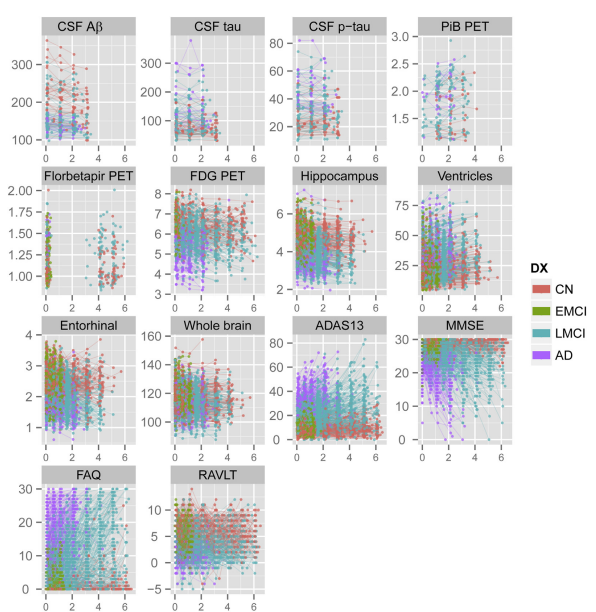
\includegraphics{fig.1}
		\caption{Iniciativa de Neuroimagen para la Enfermedad de Alzheimer (ADNI): biomarcadores, evaluaciones, categorías diagnósticas, datos longitudinales.}
		\label{fig:figura1}
	\end{figure}
	
	Se destaca la asociación entre la acumulación de placas de amiloide en el cerebro y la disminución del líquido cefalorraquídeo (CSF), junto con un aumento en la captación de PiB y florbetapir en la tomografía por emisión de positrones (PET). Se utiliza un enfoque de suavizado basado en B-spline para estimar las curvas de progresión a largo plazo, brindando una visualización clara de la evolución de la enfermedad en diferentes cohortes.\\
	
	El estudio también investiga subgrupos de sujetos, incluyendo aquellos con evidencia de acumulación de amiloide y portadores del alelo $\epsilon$4 de la apolipoproteína E (APOE). En \ref{fig:figura2} se presentan las trayectorias estimadas de dos grupos: aquellos sin evidencia de carga amiloide y aquellos sin el alelo $\epsilon$4 de APOE.\\
	
	\begin{figure}[h!]
		\centering
		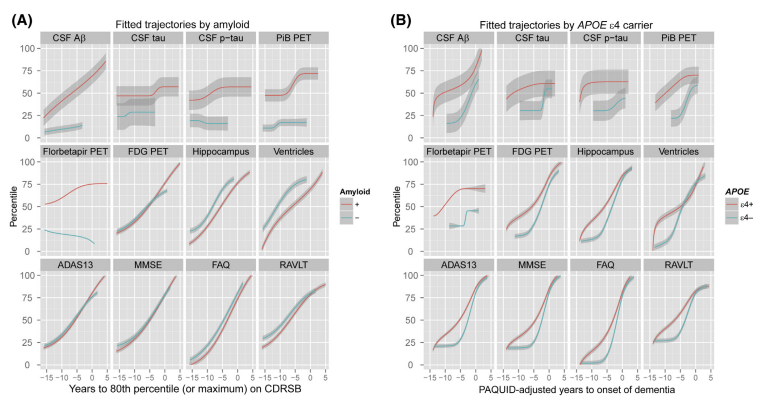
\includegraphics{fig.2}
		\caption{Comparación de portadores y no portadores del alelo APOE $\epsilon$4 en trayectorias de biomarcadores cerebrales.}
		\label{fig:figura2}	
	\end{figure}
	
	
	Se observa que los portadores de este alelo tienen una progresión más rápida de la enfermedad en comparación con los no portadores. Se emplea una transformación del tiempo para comparar las trayectorias de progresión con el estudio PAQUID, proporcionando información valiosa sobre la relación entre la carga de amiloide, la genética y la progresión clínica. 
	
	
	\subsection{Discusión}
	El texto examina la forma en que se analiza la evolución de la enfermedad de Alzheimer, utilizando datos de dos estudios: el Alzheimer's Disease Neuroimaging Initiative (ADNI) y el estudio Personnes Agées Quid (PAQUID). Se compara este enfoque con un estudio previo que se centró en cómo se hereda la enfermedad de Alzheimer, utilizando la edad en la que los padres desarrollaron síntomas para estimar la progresión de la enfermedad. Sin embargo, en este estudio, se aborda una limitación importante de ADNI al estimar tanto la edad en que se desarrollan los síntomas como las formas de evolución de la enfermedad al mismo tiempo.
	
	Además, se resaltan las diferencias en las curvas de evolución de diversos marcadores de la enfermedad, como los niveles de proteína beta-amiloide en el líquido cefalorraquídeo (CSF), la proteína tau, los resultados de tomografía por emisión de positrones (PET) con el compuesto Pittsburgh Compound B (PiB), el metabolismo de la glucosa y el tamaño del hipocampo. Se sugiere que estos marcadores siguen trayectorias distintas y que algunos tienen una evolución más constante, mientras que otros muestran un patrón de crecimiento y descenso.
	
	Por otra parte, se menciona la influencia de factores como la genética, la dieta y el estilo de vida en la variabilidad de los marcadores de la enfermedad. Se subraya la necesidad de incluir datos de grupos de estudio más jóvenes y se argumenta que la combinación de datos de múltiples fuentes ayudará a validar modelos de progresión de la enfermedad de Alzheimer en el futuro.\\
	
	
	
	\section{Modelos escalares y extensiones}
	\subsection{Geometría de Riemann}
	La geometría de Riemann es necesaria para entender las bases matemáticas que permiten definir los subespacios de características, los cuales son fundamentales a la hora de modelizar enfermedades. Para ello, es necesario explicar algunos conceptos clave. \\
	
	En primer lugar, esta geometría se basa en el concepto de variedades. Son espacios en los cuales cada punto tiene una estructura suave y diferenciable similar al espacio euclidiano. Al haber zonas de la variedad conectadas con espacios lineales, se pueden realizar cálculos diferenciables localmente. Además, si a una variedad suave \textit{M} se le equipa con una colección de productos internos $g_{\textbf{M}}=(g_{\textbf{p}})_{\textbf{p}\in \textbf{M}}$, llamados métrica en la variedad y asociados al espacio tangente $\textbf{T}_{\textbf{p}}\textbf{M}$, se le llama variedad de Riemann. Este concepto introduce la noción de distancias en la estructura diferenciable de la variedad.\\
	
	Por otra parte están las geodésicas, que son curvas que representan la trayectoria mas corta entre dos puntos en una variedad de Riemann. Son análogas a las lineas rectas en la geometría euclidiana. En el mapeo exponencial, se asocia un vector tangente a un punto con otro punto alcanzado por una geodésica a lo largo de la dirección del vector. Esto se representa con la siguiente función:
	\begin{equation}
		\textbf{v}\in\textbf{T}_{\textbf{p}}\rightarrow Exp_{\textbf{p}}(\textbf{v})=Exp_{\textbf{p},t}(\textbf{v})(t+1)
	\end{equation} 
	
	Por último, para comparar cálculos en espacios tangentes a lo largo de una geodésica, es muy importante entender el \textbf{transporte paralelo}. Teniendo una curva suave $\gamma$ y dado un vector $\textbf{w}_{0}$ en el espacio tangente $\textbf{T}_{\gamma(t_{0})\textbf{M}}$, existe un único campo vectorial paralelo a lo largo de la curva tal que $\textbf{w}(t_{0})=\textbf{w}_{0}$.\cite[Capítulo 1]{koval2020learning}
	
	\subsection{Modelo de efectos mixtos}
	Los modelos de efectos mixtos son una herramienta que permite formular la trayectoria de la progresión de una enfermedad tanto de manera global como individual, algo que no se puede hacer con la geometría de Riemann. Esto es posible combinando dos tipos efectos:
	\begin{itemize}
		\item Efectos globales o fijos: describen a la población en su conjunto. No son aleatorios.
		\item Efectos individuales o aleatorios: representan las variaciones especificas de cada observación. Son aleatorios.
	\end{itemize}
	
	A partir de los modelos de regresión clásicos, surgen dos métodos para el modelado de efectos mixtos, en función de su complejidad a la hora de capturar las interacciones entre variables de entrada y salida.
	
	
	\begin{description}
		\item {\textbf{Modelos Lineales de Efectos Mixtos (LME)}}
		
		Este modelo añade un grado de libertad más al modelo clásico de regresión lineal para capturar las variaciones especificas de cada sujeto, representándose de la siguiente manera:\\
		\begin{equation}
			\textbf{y}_{i}=\textbf{x}_{i}\alpha+\textbf{z}_{i}\beta_{i}+\epsilon_{i}
		\end{equation}
		
		donde $\textbf{y}_{i}$ son la variables de resultado de la i-ésima observación, $\textbf{x}_{i}$ y $\textbf{z}_{i}$ son las entradas, los efectos fijos son $\alpha$ y los aleatorios de cada observación se corresponden con $\beta_{i}$.
		
		\item{\textbf{Modelos No Lineales de Efectos Mixtos (NLMEM)}}
		
		Este modelo captura interacciones complejas entre las entradas y la salida. Su funcionamiento se representa con la siguiente ecuación:
		\begin{equation}
			\textbf{y}_{i}=g(\textbf{x}_{i},\textbf{z}_{i})+\epsilon_{i}
		\end{equation}
		siendo \textit{g} una función no lineal de las variables de entrada.
	\end{description}
	
	Para describir la evolución de los datos longitudinales en el caso de fenómenos biológicos, se utiliza el modelo de pendiente aleatoria e intersección aleatoria. Describe la trayectoria de cada individuo en cada visita como una variación de pendiente e intersección con respecto a la trayectoria global y se representa con la siguiente función:
	\begin{equation}
		\textbf{y}_{ij}=(\alpha^{1}+\beta_{i}^{1})t_{ij}+(\alpha^{2}+\beta_{i}^{2})+\epsilon_{ij}
	\end{equation}
	
	donde los efectos fijos de la trayectoria promedio son $\alpha^{1}$ (pendiente) y $\alpha^{2}$ (intersección) y los efectos aleatorios de cada sujeto se representan con $\beta_{i}^{1}$ (pendiente) y $\beta_{i}^{2}$ (intersección).\\
	
	Este modelo se utiliza en casos en los que los eventos de los pacientes están alineados temporalmente. Por ello, para casos como el de la progresión de una enfermedad es necesario realizar una reparametrización del tiempo ajustando las observaciones individuales con un desplazamiento temporal ($t \rightarrow t-\tau_{i}$).
	
	\subsection{Modelo de Progresión de la Enfermedad (DPM)}
	En este apartado, se presenta un modelo de efectos mixtos con el cual se pretende definir la progresión general de la enfermedad así como la trayectoria especifica de cada individuo. Esto se consigue mediante el estudio de las medidas tomadas durante las visitas sucesivas de cada uno de los pacientes.\\
	
	Para ello, cada observación tomada es considerada como parte de una variedad de Riemann y la progresión general de la enfermedad se representa con una geodésica (trayectoria promedio $\tau_{0}$). Además, las trayectorias individuales son modeladas como desviaciones espaciotemporales de la curva promedio en términos de dirección y velocidad. Teniendo la dirección definida en el desplazamiento espacial ($w_{i}$), la trayectoria individual se representaría con la siguiente función:
	\begin{equation}
		\eta^{\textbf{w}_{i}}(t):=\exp_{\gamma_0(t)} (P_{\gamma_0,t_0,t}(\textbf{w}_i)))
	\end{equation}
	
	Mientras que la progresión temporal individual ($\eta^{\textbf{w}^{i}}(t)$) se ajusta con la siguiente reparametrización temporal:
	\begin{equation}
		\psi_i:t \rightarrow \alpha_i(t - \tau_i - t_0) + t_0
	\end{equation}
	
	siendo $\alpha_i$ la aceleración, la cual indica una progresión mas rápida cuando es mayor que 1; y $\tau_{i}$ el desplazamiento temporal el cual indica una progresión más tardía cuando es menor que 0.\\
	
	Las mediciones de cada individuo \textit{i} en el tiempo \textit{j} se definen como:
	\begin{equation}
		\textbf{y}_{ij}=\eta^{\textbf{w}_{i}}(\psi_{i}(t_{ij}))+\epsilon_{ij}
	\end{equation}
	
	Estadísticamente, se puede comparar con un modelo de efectos mixtos donde la geodésica fija dentro de la configuración Riemannieana que modela la trayectoria promedio representarían los efectos fijos. Los efectos aleatorios serían las curvas individuales que se derivan de la geodésica mediante los parámetros de cada sujeto.\\
	
	Además, es necesario asegurar las condiciones de identificabilidad del modelo. Cuando haya variabilidad espaciotemporal, se utiliza el método Householder para que el producto interno entre cada columna de la matriz A y $v_{0}$ debe sea cero y así garantizar que $\textit{w}_{i}$ sea ortogonal a la velocidad $v_{0}$.\\
	
	A parte, en el modelo utilizado, la trayectoria general es percibida como un conjunto de trayectorias individuales en diferentes direcciones calculadas juntando la velocidad con unos ajustes concretos para cada observación \textit{j}.\\
	
	\begin{table}[h]
		\begin{adjustbox}{width=\textwidth}
			\begin{tabular}{|l||l|}
				\toprule
				GRÁFICAS & FUNCIONES\\
				\hline
				\multicolumn{2}{ |l| }{(a) Lineas rectas paralelas} \\
				\hline
				\raisebox{-0.6\height}{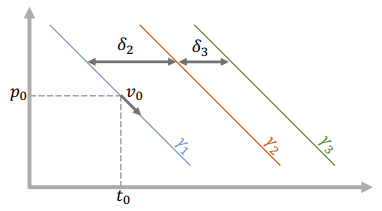
\includegraphics[width=3cm]{im1}} & \begin{tabular}{@{}l@{}} $g_p^k(u, v) = uv$ \\
					$\gamma_k(t) = p_0 + (t - t_0 - \delta_k)v_0$ \\
					$\eta_{k}^{\textbf{w}_{i}}(\psi_{i}(t_{ij})) = w_{ik} + p_{0} + (\alpha_{i}(t_{ij}-t_{0}-\tau_{i})+\delta_{k})v_{0}$ \end{tabular}\\
				\hline
				\multicolumn{2}{ |l| }{(b) Lineas rectas} \\
				\hline
				\raisebox{-0.6\height}{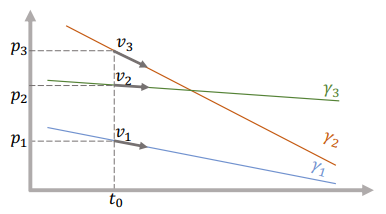
\includegraphics[width=3cm]{im2}} & \begin{tabular}{@{}l@{}} $g_p^k(u, v) = uv$ \\
					$\gamma_k(t) = p_k + (t - t_0)v_k$ \\
					$\eta_{k}^{\textbf{w}_{i}}(\psi_{i}(t_{ij})) = w_{ik} + p_{k} + \alpha_i(t_{ij}-t_{0}-\tau_{i})v_{k}$\end{tabular} \\
				\hline
				\multicolumn{2}{ |l| }{(c) Formas logísticas paralelas} \\
				\hline
				\raisebox{-0.6\height}{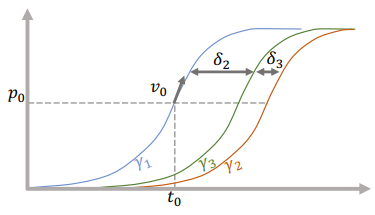
\includegraphics[width=3cm]{im3}} & \begin{tabular}{@{}l@{}} $g_p^k(u, v) = \frac{uv}{p^{2}(1-p)^{2}}$ \\
					$\gamma_k(t) = (1+(\frac{1}{p_{0}}-1)E(t))^{-1}$ \\
					$\eta_{k}^wi(\psi_i(t_{ij})) = (1+(\frac{1}{p_{0}}-1)\exp (\frac{-v_{0}(\alpha_{i}(t-\tau_{i}-t_{0})+\delta_{k})}{p_{0}(1-p_{0})}-\frac{w_{ik}(1+gE(t_{0}))^{2}}{gE(t_{0})}))^{-1}$\end{tabular} \\
				\hline
				\multicolumn{2}{ |l| }{(d) Formas logísticas} \\
				\hline
				\raisebox{-0.6\height}{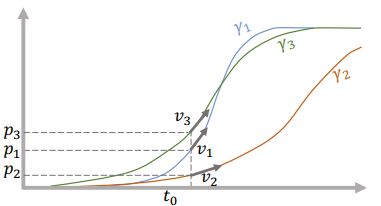
\includegraphics[width=3cm]{im4}} & \begin{tabular}{@{}l@{}} 
					$g_p^k(u, v) = \frac{uv}{p^{2}(1-p)^{2}}$\\
					$\gamma_k(t) = (1+(\frac{1}{p_{k}}-1)\exp(-\frac{v_{k}}{p_{k}(1-p_{k})}(t-t_{0})))^{-1}$ \\
					$\eta_{k}^wi(\psi_i(t_{ij})) = (1+(\frac{1}{p_{k}}-1)\exp (-\frac{w_{ik}+v_{k}\alpha_{i}(t_{ij}-\tau_{i}-t_{0})}{p_{k}(1-p_{k})}))^{-1}$\end{tabular} \\
				\hline
				\multicolumn{2}{ |l| }{(e) Decaimientos exponenciales paralelos} \\
				\hline
				\raisebox{-0.6\height}{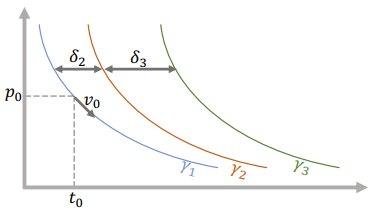
\includegraphics[width=3cm]{im5}} & \begin{tabular}{@{}l@{}} 
					$g_p^k(u, v) = \frac{uv}{p^{2}}$ \\
					$\gamma_k(t) = p_{0}\exp(-\frac{v_{0}}{p_{0}}(t-t_{0}+\delta_{k}))$ \\
					$\eta_{k}^wi(\psi_i(t_{ij})) = p_{0}\exp(-\frac{w_{i}k}{p_{0}}-\frac{v_{0}}{p_{0}}(\alpha_{i}(t_{ij}-t_{0}-\tau_{i})+\delta_{k}))$\end{tabular} \\
				\hline
				\multicolumn{2}{ |l| }{(f) Decaimientos exponenciales} \\
				\hline
				\raisebox{-0.6\height}{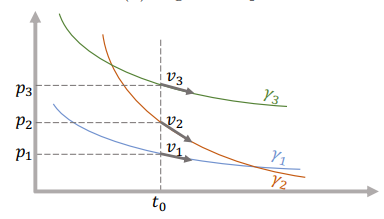
\includegraphics[width=3cm]{im6}} & \begin{tabular}{@{}l@{}} 
					$g_p^k(u, v) = \frac{uv}{p^{2}}$ \\
					$\gamma_k(t) = p_{k}\exp(-\frac{v_{k}}{p_{k}}(t-t_{0}))$ \\
					$\eta_{k}^wi(\psi_i(t_{ij})) = p_{k}\exp(-\frac{w_{ik}}{p_{k}}-\frac{v_{k}\alpha_{i}}{p_{k}}(t_{ij}-t_{0}-\tau_{i}))$\end{tabular} \\
				\bottomrule
			\end{tabular}
		\end{adjustbox}
		\caption{Instanciaciones del modelo genérico}
		\label{tab:tabla1}
	\end{table}
	
	
	\subsection{Modelo de Progresión de la Enfermedad (DPM)}
	En la tabla \ref{tab:tabla1} vemos seis distintas formas de instanciar el modelo genérico: 
	\begin{enumerate}
		\item \textbf{Lineas rectas paralelas.} Cada geodésica \textit{k} realiza una traslación horizontal de valor $\delta_{k}$ y alcanzan el valor $p_{0}$ con velocidad $v_{0}$ y tiempo $t_{0}+\delta_{k}$.
		\item\textbf{ Lineas rectas.} Representan geodésicas que alcanzan el valor $p_{k}$ con velocidad $v_{k}$ en el tiempo $t_{0}$.
		\item \textbf{Formas logísticas paralelas.} \textit{K} dimensiones representadas por curvas logísticas con valores entre 0 y 1, retrasadas por un tiempo $\delta_{k}$ y que alcanzan $p_{0}$ en el tiempo $t_{0}$ con velocidad $v_{0}$.
		\item \textbf{Formas logísticas.} Cada coordenada es independiente, alcanzando el valor $p_{k}$ en el tiempo $t_{0}$ con velocidad $v_{k}$.
		\item \textbf{Decaimientos exponenciales paralelos.} Geodésicas como curvas exponenciales decrecientes que van desde $-\infty$ finalizando en 0, trasladadas las curvas \textit{k} un tiempo $\delta_{k}$.Alcanzan $p_{0}$ con $v_{0}$ en t igual a $t_{0}$.
		\item \textbf{Decaimientos exponenciales.} Alcanzan el valor $p_{k}$ en el tiempo $t_{0}$ con velocidad $v_{k}$.
	\end{enumerate}
	
	En cada uno de ellos se refleja la función de $g_{p}^{k}$, la ecuación de la geodésica de una dimensión $\gamma_{k}$  y la coordenada k de la trayectoria individual $\eta_{k}^{\textbf{w}_{i}}(\psi_{i}(t_{ij}))$. \\
	
	Para cambiar estos seis modelos se pueden realizar algunas variaciones disponibles en softwares como Leaspy. Entre ellas encontramos las siguientes:
	\begin{itemize}
		\item Parametrización de formas distintas aplicables a los distintos modelos: valor $p_{0}$ alcanzado con velocidad $v_{0}$ en distintos momento, o valores $p_{1}$ a $p_{n}$ alcanzados por un solo momento.
		\item Modelos univariantes en los que establecer $\textbf{w}_{i}=(\textbf{w}_{i1})=0$ para poder usar los modelos mencionados.
		\item Número de fuentes ($\textit{N}_{S}$) las cuales definen el subespacio de posibles direcciones para el desplazamiento espacial. El valor ideal de esta variable es el mínimo que consigue saturar el ruido.
	\end{itemize}
	
	Una vez conocemos las distintas opciones de modelos posibles, es necesario saber como reconocer cual es el que mejor cumple las necesidades. Entre los factores a considerar están el proceso biológico en cuestión, el número de sujetos del estudio y el numero de puntos temporales disponibles en los datos. Tener en cuenta todo esto es necesario para escoger un modelo que represente con precisión la población estudiada y su evolución.\\
	
	
	
	
	
	\section{Estimation}
	\subsection{Aprendizaje estadístico y algoritmos}
	En primer lugar, el siguiente modelo correspondiente al i-ésimo sujeto, representa la dependencia de su variable de salida ($y_{i}$) en función de las variables aleatorias del mismo ($z_{i}$) y de los parámetros del modelo($\theta$). Para datos longitudinales, el grupo de observaciones en distintos momentos es $y_{i}=(y_{ij})_{j}$
	\begin{equation}
		y_{i}=f(\theta,z_{i})+\epsilon_{i}
	\end{equation}
	
	El principal objetivo es maximizar la verosimilitud buscando los parámetros que mejor describan las observaciones. Para ello, se desarrollaron diferentes algoritmos que se encargan de estimar los parámetros de modelos estadísticos. Cada uno centrado en resolver desafíos específicos utilizando enfoques iterativos:
	
	\begin{description}
		\item {\textbf{Algoritmo E-M: }}Expectation-Maximization.\\
		Debido a la dependencia con variables latentes \textit{z}, que suelen ser desconocidas, es complicado maximizar la verosimilitud directamente. Para solucionar esto, con este algoritmo se itera alternando entre el paso de Expectación, encargado de calcular a partir de $\theta(0))$  la expectativa de las variables latentes, y el paso de Maximización, que haya los parámetros $\theta(k)$ para maximizar la función anterior.
		
		\item {\textbf{Algoritmo SAEM: }}Stochastic Approximation Expectation Maximization.\\
		Desarrollado debido a la difícil optimización de la verosimilitud en modelos no lineales con variables latentes. Consiste en sustituir el paso de Expectación del algoritmo anterior por el de Aproximación Estocástica. En este se utilizan muestras $z^{k}$ para acercarse a la cantidad deseada. Además, tiene una fase de "quemado" al inicio, que opera con:
		\begin{equation}
			\mathcal{Q}_{k}(\theta)=log\ p(y,z^{(k)};\theta)
		\end{equation}
		
		crucial para explorar el espacio de soluciones. También realiza la actualización iterativa de los parámetros.
		
		\item {\textbf{Algoritmo MCMC-SAEM: }}Monte Carlo Markov Chain SAEM.\\
		Surge debido la posibilidad de que $p(z|y;\theta^{(k)})$ sea desconocida. Mediante el teorema de Bayes, se expresa en función de términos del modelo, del valor previo de variables ocultas y una constante de normalización.
		\begin{equation}
			p(\mathbf{z}|\mathbf{y};\theta^{(k)})=\frac{p(\mathbf{y}|\mathbf{z};\theta^{(k)})p(\mathbf{z};\theta^{(k)})}{p(\mathbf{y};\theta^{(k)})}
		\end{equation}
		Para solucionar esto, primero se realiza la aproximación de las muestras $z^{(k+1)}$  que sigan la distribución $p(z^{(k)}|y;\theta^{(k)})$, con el algoritmo de Metropolis-Hasting mediante el método de cadena de Markov. También se sustituye el procedimiento de muestreo por el MCMC y se hace converger hacia un punto crítico de verosimilitud observada $p(y|z)$ con el algoritmo de MCMC-SAEM. Para simplificar el logaritmo de verosimilitud se establece que el modelo pertenece a la familia exponencial. Además, solo se calcula y propaga el vector $\mathit{S}(\mathbf{y},\mathbf{z})$ para lograr una reducción computacional y se actualizan los parámetros $\theta^{(k+1)}$ en la Maximización. \cite[Capítulo 2]{koval2020learning}
		
		\item {\textbf{Algoritmo Hasting Metropolis within Gibbs sampler }}\\
		En el caso de variables multivariadas se puede complicar el muestreo de $z^{(k)}$ mediante cadena de Markov. Por ello, se desarrolló este algoritmo en el que $\mathbf{z}=(\mathbf{z}_{l})_{1\leq l\leq L}$ y $p(\mathbf{z}_{l}|\mathbf{z}_{\bar{l}}, \mathbf{y};\theta)$ es conocida hasta una constante $(\mathbf{z}_{\bar{l}}=\mathbf{z} \backslash \{{\mathbf{z}_{l}}\})$, pudiendo muestrear las coordenadas de $\mathbf{z}$. Al realizar el muestreo utilizando el muestreador de Hastings-Metropolis se llega al algoritmo de Hastings-Metropolis dentro del muestreador de Gibbs.
	\end{description}
	
	\subsection{Estimación del modelo de progresión de la enfermedad}
	En la siguiente ecuación, se ve un modelo de efectos mixtos de progresión espacio-temporal parametrizado por $\theta_{geom}$ (parámetros geométricos) y $z_{i}$ (variables ocultas individuales de la variación en la progresión promedio grupal). Estas últimas dan lugar a un conjunto global de parámetros $\theta=(\theta_{geom}, \theta_{\mathbf{z}})$.
	\begin{equation}
		y_{ij}=f(\theta_{geom},\mathbf{z}_{i},t_{ij})+\epsilon_{ij}
	\end{equation}
	
	donde:
	\begin{equation}
		\epsilon_{ij} \sim \mathcal{N}(0, \gamma^{2})
	\end{equation}
	
	La verosimilitud del modelo se formula de la siguiente forma:
	\begin{equation}
		p(\mathbf{y};\theta) = \int p(\mathbf{y}|\mathbf{z};\theta)p(\mathbf{z};\theta)dz
	\end{equation}
	
	A raíz de esto, se caracterizan los siguientes procesos estadísticos:
	\begin{description}
		\item {\textbf{Calibración.}}\\
		En esta fase, el objetivo es calcular los parámetros $\hat{\theta}$ para maximizar la verosimilitud del modelo de progresión de la enfermedad y su variabilidad. Para converger hacia un máximo local en la distribución posterior, se usa el algoritmo MCMC-SAEM (variables ocultas desconocidas y supuesto modelo de familia exponencial). \\
		
		Para este proceso, es importante tener en cuenta lo siguiente:
		\begin{itemize}
			\item Identificabilidad estructural: asegura que no haya varios grupos de parámetros generando la misma distribución.
			\item Identificabilidad práctica: Está relacionado con la calidad y la cantidad de las medidas. Para afrontar problemas en esta parte de nuestro modelo, se realiza una reparametrización.
		\end{itemize}
		\item {\textbf{Personalización.}}\\
		Consiste en maximizar la verosimilitud:
		\begin{equation}
			p(\mathbf{y}_{i}, \mathbf{z}_{i};\hat{\theta})=p(\mathbf{y}_{i}| \mathbf{z}_{i};\hat{\theta})p( \mathbf{z}_{i};\hat{\theta})
		\end{equation} 
		
		calculando el mejor valor de los efectos aleatorios $\mathbf{z}_{i}^{*}$, teniendo en cuenta un conjunto de datos longitudinales \textit{\textbf{y}} y $\hat{\theta}$ que maximiza $p(\mathbf{y},\theta)$. Dos procedimientos utilizados para la optimización son el método L-BFGS o el método de Powell. Otra alternativa es iterar \textit{K} veces con los parámetros individuales el algoritmo MCMC-SAEM.\\
		
		Que el individuo personalizado pertenezca o no al conjunto de calibración deriva en la práctica en resultados similares. Por otra parte, a mayor numero de observaciones del sujeto, mayor es la posibilidad de las mediciones individuales difieran del promedio del grupo.	
		
		\item {\textbf{Reconstrucción, imputación de valores faltantes y predicción.}}\\
		Una vez obtenida la trayectoria espacio-temporal individual, a partir de $\mathbf{z}_{i}^{*}$ devuelto por el proceso de personalización, se realiza uno de los siguientes procesos dependiendo del rango de tiempos con el que se trabaje:
		\begin{itemize}
			\item Reconstrucción ($t_{i1}<t<t_{ik_{i}}$): Reconstruye los dato del modelo $y_{ij}^{*}=f(\theta, \mathbf{z}_{i}^{*}, t_{ij})$, apareciendo un error $||y_{ij}-y_{ij}^{*}||$.
			\item Imputación de valores faltantes ($t_{i1}<t<t_{ik_{i}}$ y $t \notin \{t_{i1},...,t_{ik_{i}}\}$): Calcula valores que no se han encontrado en el conjunto inicial $y_{ij}^{*}=f(\theta, \mathbf{z}_{i}^{*}, t_{ij})$.
			\item Predicción ($t>t_{ik_{i}}$): Calcula las medidas en tiempos futuros, cuya precisión se basa en querer traspasar el escenario a largo plazo grupal a cada individuo. Es poco realista predecir etapas que estén fuera de la base de datos de entrenamiento, por ser dinámicas desconocidas.
		\end{itemize}
		
		\item {\textbf{Simulación.}}\\
		Por último, tras haber obtenido los parámetros óptimos $\hat{\theta}$ y las variables ocultas individuales, se realiza este procedimiento para simular sujetos virtuales. Esto permite crear cohortes con mayor numero de pacientes, de visitas y una mayor precisión temporal. Para saber la calidad de la cohorte simulada la comparamos con la distribución de las variables ocultas y las salidas finales de la cohorte original. Esta funcionalidad también permite corregir sesgos, como por ejemplo el incluir preferentemente pacientes con más visitas. 
	\end{description}
	
	
	
	\section{Estimation of the Disease Progression Model}
	
	Para el análisis de datos con estructura espacial con el objetivo de estimar el
	avance de enfermedades, así como para el estudio de datos longitudinales se
	desarrollaron las siguientes herramientas de software: Leasp para C++ y Leaspy
	para Python. El segundo es utilizado mayoritariamente para estimar la progresión
	de enfermedades a largo plazo, imputar valores faltantes y la simulación de
	cohortes virtuales.\cite[Capítulo 7]{koval2020learning}
	
	\subsection{Leasp: Paquete de C++ para el Análisis de Datos Longitudinales Estructurados Espacialmente}
	
	Este paquete trabaja con datos obtenidos tras la observación de pacientes a lo
	largo del tiempo. Su función se basa en: reconstruir la trayectoria a largo
	plazo de los pacientes a partir de las observaciones, ubicar cada medida de cada
	paciente en relación con la linea de tiempo promedio grupal y medir el efecto de
	ciertos cofactores como por ejemplo el género en el transcurso de la señal.\\
	
	Esta herramienta puede trabajar tanto con variables escalares, como puntuaciones
	clínicas o evaluaciones cognitivas; como con 	datos de red (PET SUVR).\\
	
	El diseño de Leasp se centra en la interacción entre un algoritmo y un modelo
	basado en entradas escalares y de red. Con esta biblioteca se tiene acceso a
	distintas carpetas que permite el uso de varias funcionalidades:
	\begin{itemize}
		\item Aplicación de procedimientos matemáticos
		\begin{itemize}
			\item Calibración
			\item Personalización
			\item Simulación
		\end{itemize}
		\item Funciones de procesamiento
		\item Herramientas de visualización
	\end{itemize}
	
	Para su correcta utilización a continuación se muestran algunas instrucciones y
	pasos que se deben seguir:
	
	\begin{description}
		\item {\textbf{Requisitos.}} Es necesario instalar las siguientes bibliotecas:
		\textit{tinyxml} (lectura y preprocesamiento de archivos xml),
		\textit{googletest} (pruebas de unidad y funcional ) y  \textit{Armadillo} (uso
		de algebra lineal para vectores y matrices) 
		
		\item {\textbf{Instalación.}} Desde la terminal, ejecutar los comandos que se
		muestran a continuación:
		\begin{enumerate}
			\item \texttt{git clone https://gitlab.com/icm-institute/aramislab/leasp}
			\item \texttt{git submodule init}
			\item \texttt{git submodule update}
			\item \texttt{. mkdir build \&\& cd build}
			\item \texttt{. cmake --options}
			\item \texttt{. make --options\}}
		\end{enumerate}
		
		\item {\textbf{Ejecución del software.}} Agregación del software a
		\texttt{/protect/T1/textdollarPATH} y ejecucion del siguiente comando:
		\begin{center}
			\texttt{leasp fit model\_stgs.xml algorithm\_stgs.xml data\_stgs.xml sampler\_stgs.xml}
		\end{center}
		
		\begin{itemize}
			\item \texttt{fit}: Ajuste de la curva promedia grupal a medidas individuales.
			\item \texttt{model\_settings}: Da información de los parámetros y del tipo de modelo	que se va a ejecutar.
			\item \texttt{algorithm\_settings.xml}: Define parámetros del algoritmo como el numero total de iteraciones.
			\item \texttt{data\_settings.xml}: Recopila la ruta de los archivos de datos.
			\item \texttt{sampler\_settings.xml}: Enumera las muestras utilizadas en el procedimiento de estimación, junto con sus parámetros.
		\end{itemize}
		
		\item {\textbf{Salidas de la estimación.}} Se producen tres archivos en el proceso: \\
		\texttt{convergence\_parameters.csv} muestra la convergencia del modelo.\\ \texttt{population\_parameters.csv} define parametros para el promedio grupal a largo plazo.\\ \texttt{individual\_parameters.csv} que son parametros temporales y espaciales para la trayectoria individual.
	\end{description}
	
	\subsection{Leaspy: Toolbox de Python para Aprender Patrones Espaciotemporales de la Progresión de la Enfermedad}
	
	Para el estudio de datos longitudinales y ver la progresión de enfermedades a largo plazo en Python se desarrollo la herramienta Leaspy. Basándose en el modelo de efectos mixtos, permite la reconstrucción de la evolución promedia e individual. Además, permite abordar problemas de los estudios de datos longitudinales, como el que cada paciente tenga un numero de observaciones distinto, permite trabajar con valores faltantes y medidas de datos estructurados espacialmente (imágenes o redes), gracias a la geometría de Riemann. También es de gran utilidad trabajando con medidas en un periodo de tiempo corto, cuando el fenómeno de estudio es de larga duración. Otras aplicaciones permiten predecir puntos temporales futuros y simular nuevas cohortes a partir de los parámetros obtenidos de un ya existente. La calidad del paquete se garantiza mediante pruebas unitarias, control de versiones git e integración continua.\\
	
	El siguiente modelo, basado en efectos mixtos, representa un conjunto de datos longitudinales $y=(y_{ij},t_{ij})\ 1 \leq i \le n, 1 \le j \le k_{i}$ de $\textit{n}$ pacientes. El número de observaciones de cada individuo $i$ se representa con $k_{i}$, siendo los tiempos de cada observación $t_{i1} < ... < t_{ik_{i}}$.
	
	\begin{equation}
		y_{ij} = f(\theta_{geom}, z_{i}, t_{ij} ) + \epsilon_{ij}
	\end{equation}
	
	$\theta_{geom}$ son los parámetros del modelo, $z_{i}$ es la variación de cada individuo respecto a la trayectoria promedio grupal y $\epsilon_{ij}$ es un ruido gaussiano. El objetivo es calcular los parámetros anteriores que hagan que los datos sean lo más verosímiles posibles. Con Leaspy se pueden realizar los siguientes procedimientos:
	\begin{enumerate}
		\item Calibración: consiste en estimar $y$ a partir de $\theta$, obteniendo la curva promedio del grupo a largo plazo. Esta basada en el algoritmo MCMC-SAEM y la varianza adaptativa y el descenso de gradiente mejoran la velocidad de convergencia.
		\item Personalización: Teniendo $\hat{\theta}$, se reconstruyen las trayectorias individuales obteniendo la variable oculta $z_{i}^{*}$. Este procedimiento estadístico incluye métodos Powell y L-BFGS.
		\item Reconstrucción, imputación de valores faltantes y predicción: Con las variables resultantes de los dos pasos anteriores, se calcula $y_{ij}^{*}=f(\hat{\theta}, z_{i}^{*}, t_{ij})$ para distintos periodos de tiempo.
		\item Simulación: Se genera un individuo completamente nuevo ($z_{i}^{0}$) a partir de $\hat{\theta}$ y un conjunto de variables individuales, pudiendo repetir el proceso hasta conseguir una cohorte virtual. Este método está basado en estimaciones condicionales gaussianas multivariadas y en funciones de densidad kernel.	
	\end{enumerate}
	
	La programación en Python de los cuatro procesos anteriores sigue una metodología bastante amigable para le usuario, ya que menos para la reconstrucción, el resto se estructuran de la siguiente manera:
	\begin{itemize}
		\item \textbf{Definición de parámetros:} el objeto \texttt{AlgorithmSettings} se encarga de esta función. En su llamada se fija el algoritmo que se quiere utilizar y otras variables. También se pueden cargar a través de kwargs o archivos json.
		\item \textbf{Llamada a las funciones:} tras el paso anterior, se realiza la llamada al método que se este llevando a cabo, introduciendo los parámetros definidos: \texttt{leaspy.fit(...)} para la calibración, \texttt{leaspy.personalize(...)} para personalizar el modelo, \texttt{leaspy.reconstruct(...)} para reconstruirlo y\\\texttt{leaspy.simulate(...)} para realizar una simulación.
		\item \textbf{Visualización y registro:} Leaspy también permite guardar archivos de registro y otras variables en archivos csv y json, lo que también permite volver a cargarlos en el programa; y se pueden visualizar perfiles de progresión o reconstrucciones de trayectorias.
	\end{itemize}
	
	Con todas estas herramientas, Leaspy es un entorno versátil y de fácil acceso que permite introducirse en el mundo del análisis y la interpretación de datos longitudinales a través de Python. Permite abordar tareas estadísticas gracias a los modelos y algoritmos en los que esta basado , pudiendo estimara parámetros y simular datos. Además es accesibles desde distintos sistemas operativos como Windows o Linux.
	
\section{Robust parametric modeling of Alzheimer's disease progression (Alzheimer's RPDPM)}

La enfermedad de Alzheimer (EA) es una demencia progresiva que comienza en el hipocampo, con biomarcadores en el líquido cefalorraquídeo (LCR) que pueden volverse anormales antes de que los cambios sean detectables en la tomografía por emisión de positrones (PET) o la resonancia magnética (MRI). El modelo de progresión de la enfermedad (DPM) se basa en estudios longitudinales para describir cómo evoluciona la EA, utilizando métodos paramétricos que suponen una evolución sigmoidea de los biomarcadores y enfoques más flexibles como los procesos gaussianos. Este estudio mejora el modelo propuesto por Jedynak al introducir una extensión robusta utilizando la estimación M y una función logística modificada, superando los métodos anteriores y ofreciendo un enfoque más eficaz para la investigación y el diagnóstico clínico de la EA \cite{ghazi2021robust}.\\

\subsection{Método}

El estudio propone un modelo robusto de progresión de la enfermedad basado en una función logística ajustada por estimación M para manejar valores atípicos. Este modelo estima los valores de los biomarcadores \( y_{i,j,k} \) en función de un "Disease Progression Score" (DPS) calculado a partir de la edad del sujeto. La relación entre el biomarcador y el DPS se modela como:

\begin{equation}
	y_{i,j,k} = f(s_{i,j}; \theta_k) + \sigma_k \epsilon_{i,j,k},
\end{equation}


donde \( f(s_{i,j}; \theta_k) \) es una función logística que describe la dinámica del biomarcador, y

\begin{equation} 
	s_{i,j} = \alpha_i t_{i,j} + \beta_i,
\end{equation}


es el DPS, donde \( t_{i,j} \) representa la edad, \( \alpha_i \) la tasa de progresión y \( \beta_i \) el inicio de la progresión.\\

La optimización del modelo se realiza minimizando una función objetivo que combina el ajuste de los parámetros del biomarcador y del sujeto utilizando una función de máxima verosimilitud. El proceso de optimización alterna entre el ajuste de los parámetros del biomarcador y los parámetros específicos del sujeto hasta que se alcanza la convergencia.\\

Para la predicción del valor del biomarcador y la clasificación clínica, el modelo utiliza los parámetros ajustados y una función logística para predecir los biomarcadores. La clasificación del estado clínico se realiza utilizando un clasificador bayesiano con estimación de densidad (KDE) \cite{parzen1962estimation}, calculando la probabilidad posterior con:

\begin{equation}
	p(c_i \mid s) = \frac{p(c_i) p(s \mid c_i)}{\sum_i p(c_i) p(s \mid c_i)}
\end{equation}

donde \( p(c_i) \) es la probabilidad previa y \( p(s \mid c_i) \) es la probabilidad ajustada. Este enfoque proporciona un sistema sólido y eficaz para modelar y clasificar enfermedades \cite{ghazi2021robust}.

\subsection{Configuración experimental}
\subsubsection{Datos}

El estudio utiliza datos de dos iniciativas importantes: ADNI y NACC. ADNI, lanzada en 2003, combina MRI, PET, biomarcadores y evaluaciones clínicas para estudiar la progresión del deterioro cognitivo y el Alzheimer, clasificando a los sujetos en cognitivamente normales (CN), deterioro cognitivo leve (DCL) y enfermedad de Alzheimer (EA). NACC, desde 1999, recopila datos similares y los clasifica en las mismas categorías en función del estado de la enfermedad.\\

Los datos se filtraron para eliminar valores atípicos y grandes brechas de tiempo, lo que dio como resultado 1.518 sujetos ADNI y 239 NACC con al menos una prueba cognitiva. Las mediciones de MRI volumétricas se ajustaron para corregir las diferencias en el tamaño de la cabeza mediante análisis de covarianza. Los datos se dividieron en conjuntos de entrenamiento y prueba, y se aplicó el método \textit{bootstrap} para estimar la varianza.

\subsubsection{Ajuste}
En cuanto al algoritmo, los parámetros se inicializan como \(\alpha^{(0)} = 1\) y \(\beta^{(0)} = 0\). La pendiente de las trayectorias \(\lambda\) se establece en -1 o 1, según los diagnósticos. Los parámetros de las funciones logísticas se estiman como \(\gamma_k = 1\), \(c_k = 0\) y \(b_k = \frac{a_k - d_k}{4 \lambda_k}\), y el procedimiento alterno se repite durante un máximo de 30 iteraciones.\\

Para evitar el sobreajuste, se seleccionan los valores óptimos de los parámetros en función de la pérdida de validación óptima \cite{prechelt2002early}:

\begin{equation}
	\{\alpha^*, \beta^*, \theta^*\} = \arg\min_{L_{\text{min}} \leq l \leq L_{\text{max}}} E_{\text{valid}}(l)
\end{equation}

donde \(E_{\text{valid}}(l)\) es la pérdida de validación en la \(l\)ª iteración. El número mínimo de iteraciones es 10 y el máximo es 50.

\subsubsection{Evaluación}
Entre las distintas métricas utilizadas para medir la precisión de las estimaciones realizadas mediante RPDPM ('Robust Parametric Disease Progression Modeling') se encuentran: 
\begin{enumerate}
	\item Criterio de información Bayesiano Robusto (BIC): utilizado parala selección de modelos entre los modelos robustos. \cite{9225726}
	\item Error Absoluto Medio (MAE): Mide la precisión de la trayectorio de la enfermedad estimada para los biomarcadores.
	\item Área  bajo la curva (AUC) de la característica operativa del receptor (ROC): mide el rendimiento diagnóstico.
\end{enumerate}

\begin{table}[h!]
	\centering
	\begin{tabular}{|c|c|}
		\hline
		\textbf{Nombre} & \textbf{Ecuación} \\
		\hline
		\text{BIC} & \( \text{BIC} = 2 E_{\text{train}}(L_{\text{opt}}) + Q \ln(N) \) \\
		\hline
		\text{MAE} & \( \text{MAE} = \frac{1}{N_k} \sum_{(i,j) \in N_k} \left| y_{i,j,k} - f(s_{i,j}; \theta_k) \right| \) \\
		\hline
		\text{AUC} & \( \text{AUC} = \frac{1}{n_c (n_c - 1)} \sum_{i=1}^{n_c - 1} \sum_{k=i+1}^{n_c} \frac{1}{n_i n_k} \left( SR_i - \frac{n_i (n_i + 1)}{2} + SR_k - \frac{n_k (n_k + 1)}{2} \right) \) \\
		\hline
	\end{tabular}
	\caption{Métricas de evaluación del RPDPM.}
\end{table}

siendo \(E_{\text{train}}(L_{\text{opt}})\) la pérdida de entrenamiento, \(N\) el número total de mediciones, \(Q\) el número total de parámetros, \(N_k\) es el número de mediciones para el biomarcador \(k\), \(y_{i,j,k}\) es el valor real, y \(f(s_{i,j}; \theta_k)\) es el valor estimado, \(n_c\) el número de clases, \(n_i\) el número de observaciones en la \(i\)-ésima clase y \(SR_i\) es la suma de los rangos de las probabilidades posteriores.\\

\subsection{Resultados y discusión}
El modelo propuesto se aplicó para analizar la dinámica de los biomarcadores de la enfermedad de Alzheimer utilizando datos de ADNI. Este modelo, basado en una función Stannard modificada y una función de pérdida logística, mostró un rendimiento superior en términos de BIC y NMAE, lo que justifica su uso en análisis posteriores.\\

El análisis temporal de los biomarcadores reveló que los biomarcadores de CSF, PET y RAVLT-IR aparecen antes que los de MRI y pruebas cognitivas. Los puntos de inflexión en las curvas de biomarcadores ayudaron a ordenar su aparición a lo largo de la enfermedad, aunque no detectaron anomalías tempranas.\\

El modelo también se destacó en la predicción de valores de biomarcadores y la clasificación del estado clínico, logrando un AUC de 0,931, mejorando así en precisión y robustez. En comparación con otros métodos, superó a los enfoques anteriores en AUC y MAE para ADAS-13, aunque tuvo un rendimiento menor en la predicción de volúmenes ventriculares normalizados.\\

Finalmente, el modelo mostró una buena capacidad de generalización cuando se aplicó a datos NACC, demostrando un desempeño superior a los modelos anteriores, lo que sugiere su robustez y adaptabilidad a diferentes cohortes.

\subsection{Conclusión}
El artículo presenta un modelo paramétrico robusto para modelar la progresión del Alzheimer utilizando estimación alternada con pérdida logística para manejar problemas de ajuste como valores atípicos. Este método transforma las edades en puntuaciones de progresión de la enfermedad y ajusta funciones modificadas a biomarcadores longitudinales. Los resultados demostraron que el método propuesto supera las técnicas actuales en rendimiento predictivo y se generaliza bien a diferentes cohortes. El enfoque se puede adaptar a datos de series temporales con datos faltantes y se puede utilizar con biomarcadores no monótonos. También se sugiere que en lugar de estimadores M, se pueden utilizar estimadores robustos \cite{rousseeuw2005robust}, aunque esto requiere optimizar un parámetro adicional para el recorte residual.

\section{Aportación al desarrollo del TFG}
\subsection{Neurodegeneración: Alzheimer, Parkinson y ELA}
Esta sección aporta una definición de los que son las enfermedades neurodegenerativas, explicando algunas de ellas como el Alzheimer o el Parkinson. Esto sirve para sentar un contexto dentro del estudio intentando simplificar el funcionamiento del cerebro humano.\\

También trata la importancia de la anticipación a estas enfermedades para intentar prevenir el declive cognitivo, siendo esta una de las razones principales de este proyecto. La importancia de encontrar modelos predictivos que ayuden a estimar con antelación la evolución de la enfermedad de Parkinson y la aparición del declive cognitivo. \\

\subsection{Clinical variables and biomarkers in prediction of cognitive impairment in patients with newly diagnosed Parkinson’s disease: a cohort study}
Este artículo destaca la importancia de predecir el declive cognitivo en etapas tempranas, a partir de combinaciones de biomarcadores como MoCA, APOE, UPSIT, etc.\\

Además se utiliza como base de datos la PPMI (Parkinson's Progression Markers Initiative) también utilizada para este proyecto, lo que sirve como base para conocer los marcadores o combinaciones de biomarcadores que han tenido más poder para pronosticar la enfermedad y compararlos con los resultados obtenidos en este caso. También sirve como referencia sobre el estado actual de la investigación sobre la aparición del declive cognitivo en etapas tempranas del Parkinson.

\subsection{Statistical analysis of longitudinal neuroimage data with Linear Mixed Effects models}
Este documento aporta información sobre la utilización de modelos de efectos mixtos lineales (LME) en el análisis de datos longitudinales. Esto es crucial para analizar los cambios de los marcadores entre los distintos pacientes y durante las visitas que realizan los mismos en tiempos diversos, y así poder predecir la progresión del declive cognitivo.\\

Por otro lado, compara la precisión de este método con otros como el ANOVA de medidas repetidas, resaltando la potencia estadística al utilizar el LME, lo cual se puede usar de referencia a la hora de escoger la forma para analizar los datos utilizados en el trabajo. 

\subsection{Estimating long-term multivariate progression from short-term data}
En este artículo se trata la complejidad de estimar la progresión de una enfermedad neurodegenerativa a largo plazo a partir de datos a corto plazo, concretamente centrándose en el Alzheimer. Aún así, sirve como referencia para la aplicación para la misma problemática aplicada al Parkinson, observando los distintos métodos descritos y los resultados obtenidos.\\

\subsection{Modelos escalares y extensiones}
Este texto aporta conceptos matemáticos y estadísticos fundamentales a la hora de predecir el declive cognitivo y modelar la progresión del Parkinson. Por ejemplo, aporta información sobre la geometría de Riemann, la cual define el espacio de características formado por geodésicas que sirve para analizar la evolución individual de la enfermedad.También explica el funcionamiento de los modelos de efectos mixtos, lineales y no lineales.\\

Todas estas herramientas son combinadas para el Modelado de Progresión de la Enfermedad (DPM), por lo que una explicación de los mismo aporta un conocimiento en profundidad de los métodos con los que se trabajará para así poder obtener unas predicciones más exactas.

\subsection{Estimation}
Este documento aporta información sobre distintos métodos avanzados de gestión de la incertidumbre y variabilidad de los datos, como el Expectation-Maximization (E-M) o el Monte Carlo Markov Chain SAEM (MCMC-SAEM).\\

También explica como aplicarlos a la calibración, personalización, reconstrucción e imputación de datos faltantes, procedimientos cruciales para adaptar los modelos a datos individuales y que será muy útil en este proyecto.

\subsection{Estimation of the Disease Progression Model}
Este apartado aporta información sobre las herramientas \textit{Leasp} y \textit{Leaspy}, las cuales serán fundamentales para el desarrollo de este trabajo. Permiten analizar datos longitudinales mediante la reconstrucción de trayectorias a largo plazo e imputar valores faltantes, muy útil para evaluar el avance de la enfermedad.\\

Además, el entorno de Leaspy, en el que se centrará el desarrollo del algoritmo de Python, permite reconstruir trayectorias individuales y simular nuevos sujetos, facilitando la predicción de futuros puntos temporales.

\subsection{Robust parametric modeling of Alzheimer's disease progression (Alzheimer's RPDPM)}
Con este texto se introduce la aplicación del método RPDPM para predecir la progresión de la enfermedad del Alzheimer. Utiliza una función logística ajustada mediante estimación robusta para manejar valores atípicos y realizar predicciones precisas. \\

Los resultados mostrados se usarán como referencia para comparar los obtenidos, utilizando \textit{Leaspy}, para la problemática de la predicción del declive cognitivo en el Parkinson.



\chapter{Materiales}
\section{Parkinson's Progression Markers Initiative (PPMI)} 
\begin{figure}[h]
	\centering
	
\includegraphics[width=0.3\textwidth]{imagenes/ppmi logo.PNG}
	\caption{Logo de la PPMI}
	\label{fig:ppmi}
\end{figure}

La PPMI es un estudio clínico que consiste en el seguimiento de un conjunto de individuos. Su objetivo es facilitar la investigación basada en la búsqueda de identificadores de la progresión de la enfermedad de Parkinson (EP), ya que para poder obtener tratamientos más efectivos es fundamental la detección temprana de marcadores específicos de la enfermedad y comprender su progresión. \cite{HomePark57:online}\\

Este proyecto fue lanzado en el 2010 con la colaboración de investigadores, pacientes y la Michael J. Fox Foundation (MJFF). Entre los pacientes incluidos se encuentran tanto individuos recién diagnosticados de EP, identificados dentro del grupo PD, como sujetos que no la padecen pero que tienen riesgo de de desarrollarla en el futuro, los cuales entran dentro del grupo de control HC, formado por 196 individuos.\\

Dentro del grupo de pacientes que han sido diagnosticados con Parkinson, hay tres subgrupos dentro de los cuales han sido clasificados en función del nivel de desarrollo del declive cognitivo:
\begin{itemize}
	\item PD-CU: Individuos que no presentan deterioro cognitivo. Esta compuesto por un total de 323 pacientes.
	\item PD-MCI: Individuos a los que se les ha detectado un declive cognitivo leve, siendo en total 83 pacientes.
	\item PDD: Individuos diagnosticados con demencia, son un total de 17 sujetos. 
\end{itemize}

Cada uno de los participantes permanece en el estudio durante varios años, permitiendo un seguimiento durante este tiempo en el que se toman medidas de distintos parámetros fundamentales para estudiar la progresión de la enfermedad: marcadores biológicos, evaluaciones clínicas, pruebas de imágenes cerebrales o análisis de líquido cefalorraquídeo. \cite{marek2011parkinson}\\
 
La PPMI permite que la búsqueda de biomarcadores sea más rápida y eficaz, ya que permite la colaboración entre diferentes científicos y el entendimiento de los cambios en el curso clínico entre unos pacientes u otros.


\section{Leaspy}
\label{sec:leaspy}
\begin{figure}[h]
	\centering
	
\includegraphics[width=0.3\textwidth]{imagenes/leaspyLogo.PNG}
	\caption{Logo de Leaspy}
	\label{fig:leaspy}
\end{figure}
Para el análisis de datos con estructura espacial con el objetivo de estimar el
avance de enfermedades, así como para el estudio de datos longitudinales se
desarrollaron las siguientes herramientas de software: Leasp para C++ y Leaspy
para Python. El segundo es utilizado mayoritariamente para estimar la progresión
de enfermedades a largo plazo, imputar valores faltantes y la simulación de
cohortes virtuales.

\subsection{Leasp: Paquete de C++ para el Análisis de Datos Longitudinales
	Estructurados Espacialmente}

Este paquete trabaja con datos obtenidos tras la observación de pacientes a lo
largo del tiempo. Su función se basa en: reconstruir la trayectoria a largo
plazo de los pacientes a partir de las observaciones, ubicar cada medida de cada
paciente en relación con la linea de tiempo promedio grupal y medir el efecto de
ciertos cofactores como por ejemplo el género en el transcurso de la señal. \cite{Welcomet75:online}\\

Esta herramienta puede trabajar tanto con variables escalares, como puntuaciones
clínicas o evaluaciones cognitivas; como con 	datos de red (PET SUVR).\\

El diseño de Leasp se centra en la interacción entre un algoritmo y un modelo
basado en entradas escalares y de red. Con esta biblioteca se tiene acceso a
distintas carpetas que permite el uso de varias funcionalidades:
\begin{itemize}
	\item Aplicación de procedimientos matemáticos
	\begin{itemize}
		\item Calibración
		\item Personalización
		\item Simulación
	\end{itemize}
	\item Funciones de procesamiento
	\item Herramientas de visualización
\end{itemize}

Para su correcta utilización a continuación se muestran algunas instrucciones y
pasos que se deben seguir:

\begin{description}
	\item {\textbf{Requisitos.}} Es necesario instalar las siguientes bibliotecas:
	\textit{tinyxml} (lectura y preprocesamiento de archivos xml),
	\textit{googletest} (pruebas de unidad y funcional ) y  \textit{Armadillo} (uso
	de algebra lineal para vectores y matrices) 
	
	\item {\textbf{Instalación.}} Desde la terminal, ejecutar los comandos que se
	muestran a continuación:
	\begin{enumerate}
		\item \texttt{git clone https://gitlab.com/icm-institute/aramislab/leasp}
		\item \texttt{git submodule init}
		\item \texttt{git submodule update}
		\item \texttt{. mkdir build \&\& cd build}
		\item \texttt{. cmake --options}
		\item \texttt{. make --options\}}
	\end{enumerate}
	
	\item {\textbf{Ejecución del software.}} Agregación del software a
	\texttt{/protect/T1/textdollarPATH} y ejecucion del siguiente comando:
	\begin{center}
		\texttt{leasp fit model\_stgs.xml algorithm\_stgs.xml data\_stgs.xml sampler\_stgs.xml}
	\end{center}
	
	\begin{itemize}
		\item \texttt{fit}: Ajuste de la curva promedia grupal a medidas individuales.
		\item \texttt{model\_settings}: Da información de los parámetros y del tipo de modelo	que se va a ejecutar.
		\item \texttt{algorithm\_settings.xml}: Define parámetros del algoritmo como el numero total de iteraciones.
		\item \texttt{data\_settings.xml}: Recopila la ruta de los archivos de datos.
		\item \texttt{sampler\_settings.xml}: Enumera las muestras utilizadas en el procedimiento de estimación, junto con sus parámetros.
	\end{itemize}
	
	\item {\textbf{Salidas de la estimación.}} Se producen tres archivos en el proceso: \\
	\texttt{convergence\_parameters.csv} muestra la convergencia del modelo.\\ \texttt{population\_parameters.csv} define parametros para el promedio grupal a largo plazo.\\ \texttt{individual\_parameters.csv} que son parametros temporales y espaciales para la trayectoria individual.
\end{description}

\subsection{Leaspy: Toolbox de Python para Aprender Patrones Espaciotemporales de la Progresión de la Enfermedad} \label{sec:parámetros de leaspy}

Para el estudio de datos longitudinales y ver la progresión de enfermedades a largo plazo en Python se desarrollo la herramienta Leaspy. Basándose en el modelo de efectos mixtos, permite la reconstrucción de la evolución promedia e individual. Además, permite abordar problemas de los estudios de datos longitudinales, como el que cada paciente tenga un numero de observaciones distinto, permite trabajar con valores faltantes y medidas de datos estructurados espacialmente (imágenes o redes), gracias a la geometría de Riemann. También es de gran utilidad trabajando con medidas en un periodo de tiempo corto, cuando el fenómeno de estudio es de larga duración. Otras aplicaciones permiten predecir puntos temporales futuros y simular nuevas cohortes a partir de los parámetros obtenidos de un ya existente. La calidad del paquete se garantiza mediante pruebas unitarias, control de versiones git e integración continua.
\begin{figure}[h]
	\centering
	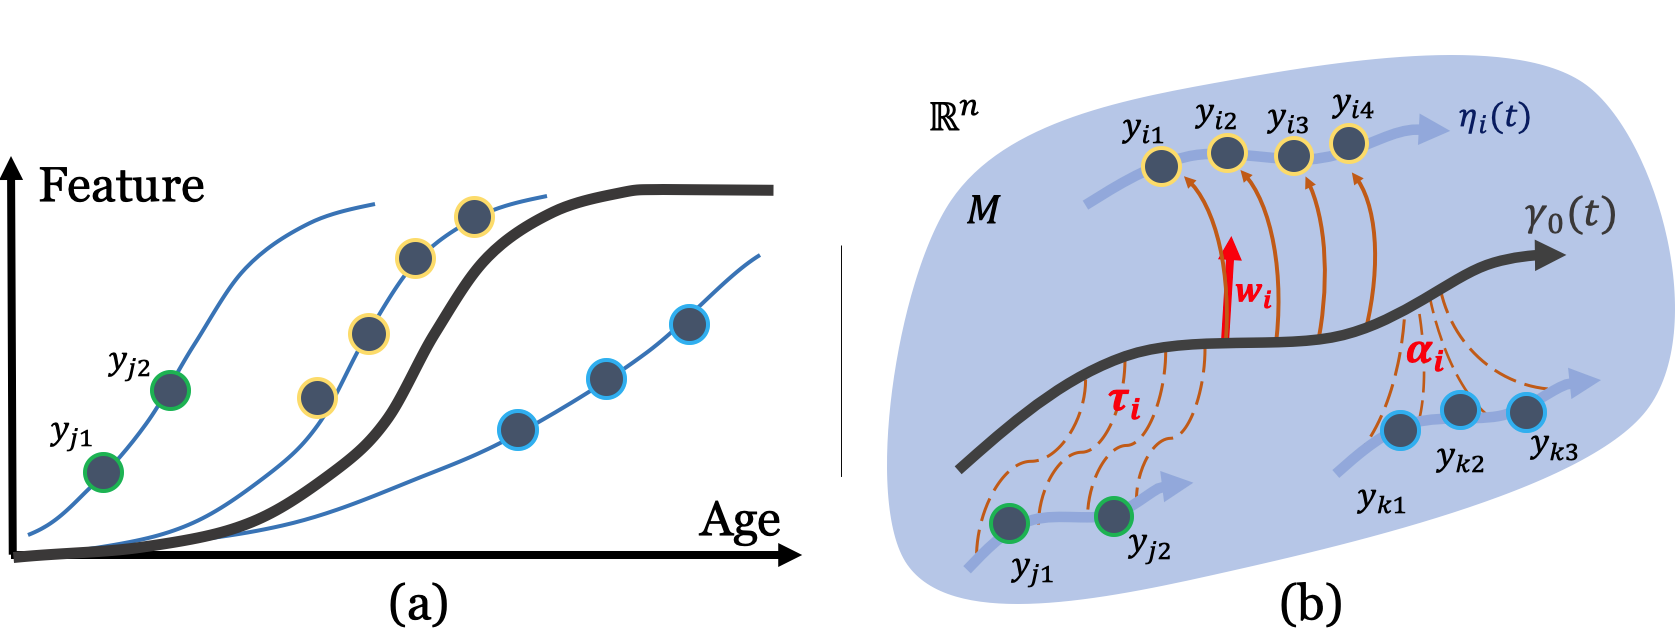
\includegraphics[width=0.9\textwidth]{imagenes/leaspy_trayectories.PNG}
	\caption{Curvas características de la progresión de los marcadores.}
	\label{fig:trayectories}
\end{figure}

El siguiente modelo, basado en efectos mixtos, representa un conjunto de datos longitudinales $y=(y_{ij},t_{ij})\ 1 \leq i \le n, 1 \le j \le k_{i}$ de $\textit{n}$ pacientes. El número de observaciones de cada individuo $i$ se representa con $k_{i}$, siendo los tiempos de cada observación $t_{i1} < ... < t_{ik_{i}}$.

\begin{equation}
	y_{ij} = f(\theta_{geom}, z_{i}, t_{ij} ) + \epsilon_{ij}
\end{equation}

$\theta_{geom}$ son los parámetros del modelo, $z_{i}$ es la variación de cada individuo respecto a la trayectoria promedio grupal y $\epsilon_{ij}$ es un ruido gaussiano. El objetivo es calcular los parámetros anteriores que hagan que los datos sean lo más verosímiles posibles. Con Leaspy se pueden realizar los siguientes procedimientos:

\begin{enumerate}
	\item Calibración: consiste en estimar $y$ a partir de $\theta$, obteniendo la curva promedio del grupo a largo plazo. Esta basada en el algoritmo MCMC-SAEM y la varianza adaptativa y el descenso de gradiente mejoran la velocidad de convergencia.
	\item Personalización: Teniendo $\hat{\theta}$, se reconstruyen las trayectorias individuales obteniendo la variable oculta $z_{i}^{*}$. Este procedimiento estadístico incluye métodos Powell y L-BFGS.
	\item Reconstrucción, imputación de valores faltantes y predicción: Con las variables resultantes de los dos pasos anteriores, se calcula $y_{ij}^{*}=f(\hat{\theta}, z_{i}^{*}, t_{ij})$ para distintos periodos de tiempo.
	\item Simulación: Se genera un individuo completamente nuevo ($z_{i}^{0}$) a partir de $\hat{\theta}$ y un conjunto de variables individuales, pudiendo repetir el proceso hasta conseguir una cohorte virtual. Este método está basado en estimaciones condicionales gaussianas multivariadas y en funciones de densidad kernel.	
\end{enumerate}

La programación en Python de los cuatro procesos anteriores sigue una metodología bastante amigable para le usuario, ya que menos para la reconstrucción, el resto se estructuran de la siguiente manera:
\begin{itemize}
	\item \textbf{Definición de parámetros:} el objeto \texttt{AlgorithmSettings} se encarga de esta función. En su llamada se fija el algoritmo que se quiere utilizar y otras variables. También se pueden cargar a través de kwargs o archivos json.
	\item \textbf{Llamada a las funciones:} tras el paso anterior, se realiza la llamada al método que se este llevando a cabo, introduciendo los parámetros definidos: \texttt{leaspy.fit(...)} para la calibración, \texttt{leaspy.personalize(...)} para personalizar el modelo, \texttt{leaspy.reconstruct(...)} para reconstruirlo y\\\texttt{leaspy.simulate(...)} para realizar una simulación.
	\item \textbf{Visualización y registro:} Leaspy también permite guardar archivos de registro y otras variables en archivos csv y json, lo que también permite volver a cargarlos en el programa; y se pueden visualizar perfiles de progresión o reconstrucciones de trayectorias.
\end{itemize}

Además, para comprender el funcionamiento de este entorno, hay que tener claros los parámetros con los que trabaja Leaspy a la hora de obtener los modelos \cite{DiseaseC47:online}. Por una parte, a la hora de estimar la trayectoria de la progresión media de un biomarcador se utilizan los parámetros \textit{'long-term'}:
\begin{itemize}
	\item $\mathbf{t_{k}}$: Edad para la cual se obtienen los parámetros  que definen la curva general (p0 y u0).
	\item $\mathbf{p_{k}}$: Indica el valor normalizado de la variable en el tiempo t0 para la trayectoria a largo plazo.
	\begin{equation}
		p_{k}=\gamma_{k}(t_{k})
	\end{equation}
	\item $\mathbf{u_{k}}$: Representa la velocidad de aumento del valor de dicha variable en función del tiempo.
	\begin{equation}
		u_{k}=\frac{d}{dt}(\gamma_{k}(t_{k}))
	\end{equation}
\end{itemize}
Estás variables permiten estimar la trayectoria global media de cada biomarcador ($\gamma_{k}$). Esto se realiza con la función \textbf{leaspy.fit}, la cual toma las medidas longitudinales de los sujetos de la base de datos y obtiene los parámetros que definen la curva \textit{'long-term'}. Una vez obtemidos los parámetros, la curva se obtiene con la siguiente ecuación:
\begin{equation}
	\gamma_{k}=\frac{1}{1+((\frac{1}{p_{k}}-1)*exp(-\frac{u_{k}*(t-t_{0})}{p_{k}*(1-p_{k})}))}
\end{equation}

\begin{figure}[h]
	\centering
	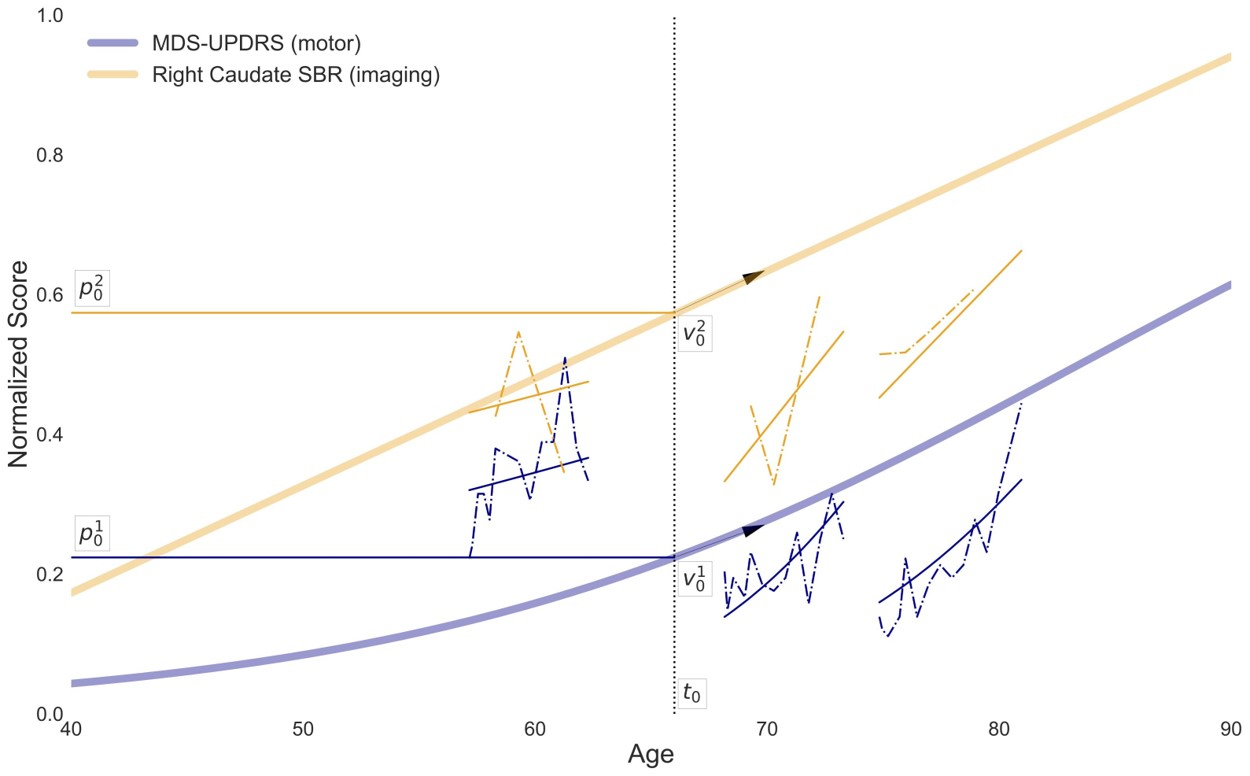
\includegraphics[width=0.85\textwidth]{imagenes/PARÁMETROS LONG TERM.JPG}
	\caption{Representación de los parámetros de una trayectoria long-term}
	\label{fig:long-term}
\end{figure}

Una vez conseguido esto, Leaspy utiliza la función \textbf{leaspy.personalize} para obtener los parámetros \textit{'short-term'}:
\begin{itemize}
	\item $\mathbf{\tau_{i}}$: Representa la reserva cognitiva en años, es decir, el tiempo del que dispone un sujeto antes de alcanzar el declive cognitivo. un valor mayor que 0 indica que la progresión de la enfermedad es más tardía que la media, en cambio un valor negativo indica que que es más temprana.
	\item $\mathbf{\alpha_{i}}$: EL factor de aceleración marca si en el caso del sujeto seleccionado, la enfermedad avanza a mayor velocidad que la media ($\alpha_{i}>1$) o a menos velocidad ($\alpha_{i}<1$).
	\item $\mathbf{w_{ik}}$: El espacio entre marcadores intermedios  indica la secuencia de eventos descrita por el vector $\tau$, que desplaza cada curva logística, propia del paciente.
\end{itemize}
Estas variables representan la curva característica para un nuevo individuo a partir de la trayectoria general obtenida de un grupo de pacientes facilitado. Esta curva se obtiene con la siguiente ecuación en función de los parámetros \textit{'short-term'}:
\begin{equation}
	\eta_k = \frac{1}{1 + \left( \left( \frac{1}{pk} - 1 \right) \cdot e^{-\frac{(w_{ik} + (u_k \cdot \alpha_i \cdot (t_{ij} - t_0 - \tau_i)))}{pk \cdot (1 - pk)}} \right)}
\end{equation}

\begin{figure}[h]
	\centering
	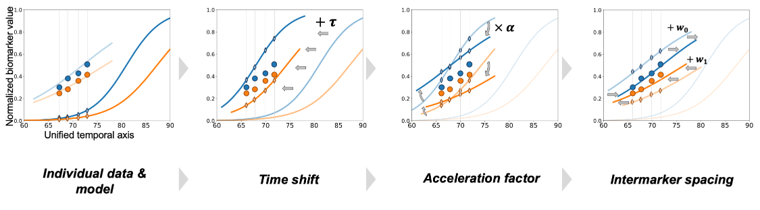
\includegraphics[width=1\textwidth]{imagenes/PARAMETROS SHORT TERM.PNG}
	\caption{Parámetros short-term para la obtención de la curva caracteristica de un nuevo sujeto.}
	\label{fig:short-term}
\end{figure}
Con todas estas herramientas, Leaspy es un entorno versátil y de fácil acceso que permite introducirse en el mundo del análisis y la interpretación de datos longitudinales a través de Python. Permite abordar tareas estadísticas gracias a los modelos y algoritmos en los que esta basado , pudiendo estimara parámetros y simular datos. Además es accesibles desde distintos sistemas operativos como Windows o Linux.

\section{Spyder}
\begin{figure}[h]
	\centering
	
\includegraphics[width=0.3\textwidth]{imagenes/logo_spyder.PNG}
	\caption{Logo de Spyder.}
	\label{fig:spyder}
\end{figure}

"The Scientific Python Development Environment", por sus siglas en inglés Spyder (cuyo logo se ve en la figura \ref{fig:spyder}), es un entorno de desarrollo integrado (IDE) escrito en Python y para Python. Es una herramienta que permite el manejo avanzado de datos, su investigación, análisis, inspección y depuración entre otras muchas acciones. \cite{IPythonC75:online} \\

Esta interfaz consta de varios componentes: 
\begin{itemize}
	\item Editor multi-lenguaje: permite generar, modificar y visualizar código en Python. Además, consta de diversas herramientas y características que facilitan su uso y dan una mayor eficiencia.
	\item \textit{IPython Console}: En este panel se pueden ejecutar comandos, se interactúa con la información y se puede \textit{ejecutar} el código por líneas, celdas o ficheros y depurar el mismo.
	\item Explorador de variables, gráficos y ayuda: En el último panel se pueden escoger distintas ventanas donde observar las variables y parámetros con los que trabaja el programa, buscar ayuda sobre distintos comandos, observar gráficos y navegar por los distintos ficheros del sistema y abrirlos directamente en el entorno.
\end{itemize}

Para este proyecto, se incluyeron varias librerías clave para la programación en este lenguaje y otras con funciones más concretas que simplificaron el desarrollo de ciertos fragmentos. Entre las más importantes se encuentran:
\begin{itemize}
	\item \textbf{NumPy}: creada concretamente para cálculo y análisis de grandes cantidades de datos. Permite trabajar con \textit{arrays} en vez de con listas de Python, lo que otorga un mayor rendimiento.
	\item \textbf{Pandas}: mejora la manipulación y el análisis de datos, integrando el tipo de datos Dataframe, manejo de datos faltantes, reestructuración y segmentación de conjuntos entre muchas otras funciones.
	\item \textbf{Matplotlib}: esta libreria es especifica para la realización de gráficos y visualización de datos. Concretamente se trabajó con el módulo \textbf{Matplotlib.pyplot}, que proporciona una interfaz de porogramación sencilla y con una interfaz gráfica muy similar a la de MATLAB.
	\item \textbf{SciPy}: incluye módulos para realizar cálculos estadísticos, optimización, integración, algebra linear, etc. Es útil para trabajar numericamente con \textit{NumPy arrays}.
	\item \textbf{Seaborn}:Crea gráficos estadísticos extendiendo y simplificando las capacidades de \textit{Matplotlib} y trabajando con estructuras de datos de \textit{pandas}.
	\item \textbf{Os}: permite interactuar con el sistema operativo. Con ella se pueden crear, eliminar y mover archivos y directorios. En este trabajo se utilizó concretamente para guardar y cargar variables en el directorio de trabajo.
	\item \textbf{Leaspy}: es un paquete de software fundamental para este proyecto, explicado en profundidad en el apartado \ref{sec:leaspy}. Utilizado para el análisis de datos médicos longitudinales.
\end{itemize}

Para acceder a este entorno se utilizó la interfaz gráfica de usuario llamada \textit{Anaconda Navigator}. Con ella, además de acceder a \textit{Spyder}  están disponibles muchos otros entornos.


\section{MATLAB}
\begin{figure}[h]
	\centering
	
\includegraphics[width=0.3\textwidth]{imagenes/matlab.PNG}
	\caption{Logo de MatLab.}
	\label{fig:matlab}
\end{figure}

MATLAB es un entorno de programación de alto nivel utilizado para el análisis de datos y cálculos numéricos, desarrollo de algoritmos y visualización de gráficos. \\

Para este proyecto, fue fundamental a la hora de visualizar distintas problemáticas desarrolladas previamente por otros investigadores. Por ejemplo, uno de los objetivos fundamentales es observar la capacidad de predicción de Leaspy en comparación con la precisión de predicción del método RPDPM (Robust Parametric Disease Progression Modeling). Para ello, se utilizó MATLAB como plataforma para observar el funcionamiento de algortimos desarrollados mediante RPDPM.
  
  
\section{PuTTY}
\begin{figure}[h]
	\centering
	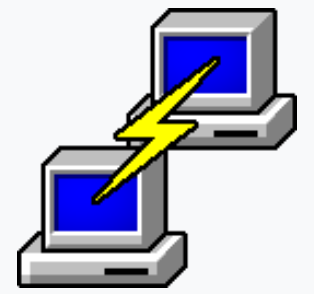
\includegraphics[width=0.2\textwidth]{imagenes/putty.PNG}
	\caption{Logo de PuTTy.}
	\label{fig:putty}
\end{figure}

PuTTy (cuyo logo se ve en la figura \ref{fig:putty}) es una herramienta utilizada para la conexión a servidores y dispositivos remotos para sistemas operativos como Windows \cite{Download87:online}.Es un cliente de terminal bastante flexible que puede utlizar distintos protocolos para realizar la conexión: SSH, Telnet, rlogin entre otros.\\ 

Para este proyecto, se usó esta herramienta para conectarse de forma segura a las máquinas Linux de supercomputación  llamadas \textit{Curie} y \textit{Magerit}, disponibles en la Universidad Politécnica de Madrid. Son destinadas para la ejecución de cargas de trabajo científico que necesitan cómputo intensivo. Para acceder a ellas de forma remota desde Putty, se utiliza el protocollo SSH (Secure SHell) el cual permite entrar de forma segura mediante un canal con la información cifrada \cite{lucas2018ssh}. Para ello, solo hay que introducir en la interfaz de este software \ref{fig:interfaz_putty} la dirección IP y el puerto de la máquina a la que quieres acceder y, posteriormente, el usuario y la contraseña en la propia terminal.\\

\begin{figure}[h]
	\centering
	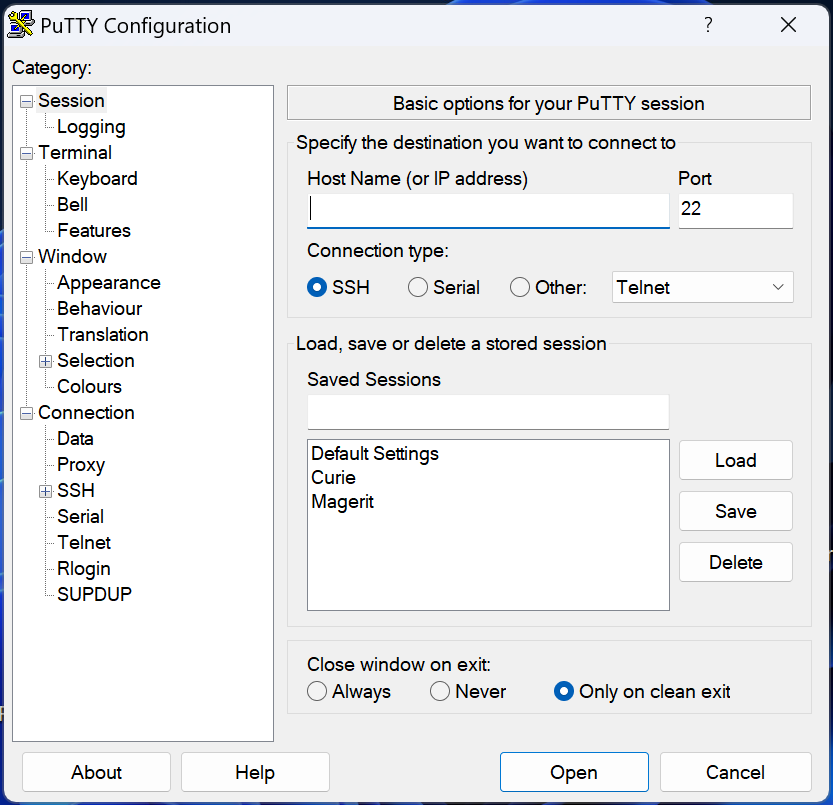
\includegraphics[width=0.5\textwidth]{imagenes/interfaz_putty.PNG}
	\caption{Interfaz de PuTTy.}
	\label{fig:interfaz_putty}
\end{figure}


\section{Xming}
\begin{figure}[h]
	\centering
	
\includegraphics[width=0.3\textwidth]{imagenes/xming.PNG}
	\caption{Logo de Xming.}
	\label{fig:xming}
\end{figure}

Xming es un servidor X para Windows que facilita el uso de aplicaciones gráficas Unix en un entorno Windows \cite{XmingXSe60:online}. Es decir, permite visualizar aplicaciones gráficas que se estén ejecutando en un servidor remoto, al cual en este casos e accede mediante SSH, mostrando las ventanas en el escritorio de Windows.\\

Para su correcto funcionamiento, lo habitual es que una vez está instalado en el dispositivo, cuando se quiera usar deberá dejarse iniciado como un servidor en segundo plano, así más adelante se pueden conectar aplicaciones gráficas desde el cliente SSH, dando acceso a software que no tiene una versión nativa para Windows.\\

Para comprobar el correcto funcionamiento de Xming, una vez lo veas abierto en segundo plano en los iconos ocultos, en la terminal de Putty se debe ejecutar el comando $\mathtt{xeyes\; \&}$ y aparecerá una ventana gráfica con unos ojos, indicando que el software se ha abierto correctamente.


\section{FileZilla Client}
\begin{figure}[h]
	\centering
	
\includegraphics[width=0.2\textwidth]{imagenes/filezilla.PNG}
	\caption{Logo de Filezilla.}
	\label{fig:filezilla}
\end{figure}

A la hora de transferir los archivos del programa desarrollado desde el directorio local al escritorio remoto para poder ejecutarlo desde las máquinas de supercomputación \textit{Curie} y \textit{Magerit}, se utilizó Filezilla Client. Esta herramienta es un cliente de FTP (Protocolo de Transferencia de Archivos) de código abierto, que se utiliza para transferir archivos de un cliente a un servidor \cite{FileZill81:online}.\\

Filezilla consta tanto con el servicio de cliente como con el de servidor, pero son descargados por separado. Desde \textit{Filezilla Client} debe concretarse la dirección del servidor al que desea conectarse para el intercambio de archivos, el usuario y la contraseña del mismo. Para este caso, se utiliza el protocolo FTP, pero \textit{Filezilla} soporta otros como el SFTP (SSH Protocolo de Transferencia de Archivos) o el FTPS (FTP Seguro), que realizan transferencias más seguras.

\section{Curie y Magerit-3}
A la hora de realizar la paralelización del código, para poder estimar el mayor número de modelos posibles de la forma más eficiente y así luego compararlos, se accedió a dos máquina de supercomputación facilitadas por la Universidad Politécnica de Madrid (UPM) y por el Centro de Supercomputación y Visualización de Madrid (CeSViMa), llamadas \textit{Curie} y \textit{Magerit}. \\

Para acceder a las mismas se utiliza la interfaz de Putty como ya se explicó anteriormente. Una vez abierta la terminal, para trabajar con Curie se utiliza la aplicación \textit{Tmux}, un multiplexor de terminales basado en sesiones. Esto permite paralelizar el programa con alto coste de computación y ejecutarlo dentro de las sesiones creadas. Ademas, permite que las distintas tareas sigan ejecutándose aunque se desconecte la sesión. \\

Por otro lado, Magerit es una infraestructura de cómputo posicionada como uno de los supercomputadores energéticamente más eficientes del mundo. Está formado por 72 nodos de propósito general \textit{ThinkSystem} SD530 con procesadores Intel Xeon Gold 6230 y 192 GiB de RAM, y 48 nodos \textit{ThinkSystem} SD530, cada uno de ellos equipado con procesadores Intel Xeon Gold 6240R y 768 GiB de RAM \cite{Descripc17:online}. En este entorno, las tareas se ejecutan mediante ficheros BASH utilizando el comando sbatch.


\section{LaTeX}
\begin{figure}[h]
	\centering
	
\includegraphics[width=0.2\textwidth]{imagenes/latex.PNG}
	\caption{Logo de LaTeX.}
	\label{fig:latex}
\end{figure}

Para la redacción del documento presente se hizo uso de la herramienta LaTeX. Es un sistema de composición de textos de alta calidad importante para generar informes científicos, técnicos y académicos \cite{LaTeXAdo12:online}.

\chapter{Métodos}

\section{Introducción}
En esta sección se explicarán los distintos procesos llevados a cabo en el estudio y predicción de la enfermedad de Parkinson en los distintos pacientes de la cohorte obtenida de la iniciativa de PPMI.\\

Para poder trabajar con ella, primero se realizaron una serie de adaptaciones para obtener un formato concreto.


\section{Estudio transversal sobre la influencia de marcadores en el declive cognitivo en la Enfermedad de Parkinson}

La enfermedad de Parkinson es una afección neurodegenerativa que afecta a un gran numero de personas en todo el mundo. Por ello, unos de los desafíos clave es el desarrollo de métodos de predicción basados en el declive cognitivo leve en etapas tempranas, ya que permitiría avanzar en la detección de la enfermedad. Para lograr esto, este estudio se centra en la búsqueda de marcadores significativos en las primeras fases de la enfermedad.\\

En primer lugar, se comparan los valores al inicio del estudio de las distintas variables, entre el grupo de pacientes a los que se les ha diagnosticado Parkinson (PD) con el grupo de control formado por pacientes sanos (HC). Esto se consigue calculando el post-hoc de cada variable, ya que indicará que variables son o no determinantes.\\

En la segunda tabla, se dividen los pacientes PD en función de como avancen durante el transcurso de la enfermedad, separándose en: cognitivammente normales (PD\_CU), pacientes con deterioro cognitivo medio (PD\_MCI) y pacientes que desarrollaron demencia (PDD), como se puede ver en la tabla \ref{tab:tabla4}. Con esto se pretenden encontrar los indicadores del avance de la enfermedad a estos grupos.\\

\begin{table}[t]
	\centering
	\begin{tabular}{|c||c|c|} 
		\hline
		\multicolumn{3}{|c|}{Clasificación general} \\
		\hline
		- &  Nº Pacientes &  Porcentaje\\ 
		\hline
		TOTAL &  683 & 100\% \\
		\hline
		PD & 423 &  61,9\%  \\
		\hline
		HC & 196  &  28,7\%  \\
		\hline
		\multicolumn{3}{|c|}{Subclasificacion grupo PD} \\
		\hline
		- &  Nº Pacientes &  Porcentaje\\
		\hline
		PD-CU &  323 &  47,3\%  \\
		\hline
		PD-MCI &   83 &   12,2\% \\
		\hline
		PDD &  17 &  2,5\%  \\ 
		\bottomrule
	\end{tabular}
	\caption{División del grupo de pacientes en función del estado de la enfermedad}
	\label{tab:tabla4}
\end{table}


Para realizar ambas tablas y los estudios estadísticos se llevaron a cabo algoritmos de análisis de datos en Python ubicados en las siguientes direcciones:
\begin{center}
	\texttt{Demos/rroca\_python/Tabla1\_python/tabla1.py}\\
		
	\texttt{Demos/rroca\_python/Tabla1\_div\_PD/tabla1\_div\_PD\_int2.py}
\end{center} 

En el primer directorio se ubica el programa encargado de generar la tabla de comparación de las características clínicas y demográficas de los pacientes de control y con enfermedad de Parkinson. En el segundo directorio, se genera la tabla que compara el avance de los pacientes con Parkinson a los distintos grupos clínicos al inicio del estudio.\\

Su diseño se baso en la interpretación y procesamiento de los datos de pacientes con Enfermedad de Parkinson y de un grupo de control,  recopilados dentro de la cohorte de PPMI (Parkinson's Progression Markers Initiative). Entre las funciones clave dentro del código se incluyeron:

\begin{description}
	
	\item {\textbf{Función de Chi-Cuadrado}} 
	
	Utilizada para evaluar la relación entre las variables categóricas como se ve en la tabla \ref{tab:tabla5} y la presencia o ausencia de declive cognitivo. Estas variables representan grupos o categorías, como el género ("Female") y el APOE4. Con este proceso se averiguó cuales de ellas estaban significativamente asociadas con el deterioro cognitivo.\\
	
	\begin{table}[t]
		\centering
		\begin{tabular}{|c|c|c|} 
			\toprule
			Variable dependiente (y) & \multicolumn{2}{|c|}{Variable independiente (x)} \\
			\hline
			- &  Continua &  Categórica\\ 
			\hline
			Continua &  Regresión & ANOVA \\
			\hline
			Categórica & Regresión logística &  Test Chi-Cuadrado  \\
			\bottomrule
		\end{tabular}
		\caption{Técnicas estadísticas de análisis de distintos tipos de variables}
		\label{tab:tabla5}
	\end{table}
	
	\begin{algorithm}
		\caption{chi\_square\_with\_posthoc}
		\begin{algorithmic}[1]
			\REQUIRE $group1, group2, group3, contingency\_table, i, v$
			\ENSURE $post\_hoc$ (String) y modificación de $data\_nm["p-value"][i+1]$
			\STATE $chi2, p\_value, dof, expected \leftarrow chi2\_contingency(contingency\_table)$
			\STATE \textbf{print} $p\_value$
			\IF{$p\_value < 0.01$}
			\STATE $data \leftarrow np.concatenate([group1, group2, group3])$
			\STATE $labels \leftarrow ['group1'] * len(group1) + ['group2'] * len(group2) + ['group3'] * len(group3)$
			\STATE $tukey\_results \leftarrow pairwise\_tukeyhsd(data, labels, 0.01)$
			\STATE $possible\_results \leftarrow ['a', 'b', 'c']$
			\STATE $post\_hoc \leftarrow []$
			\FOR{$res, reject$ \textbf{in} \textbf{zip}($possible\_results, tukey\_results.reject$)}
			\IF{$reject$ \textbf{is} \textbf{True}}
			\STATE $post\_hoc$.append($res$)
			\ENDIF
			\ENDFOR
			\STATE $post\_hoc \leftarrow$ \textbf{join}($post\_hoc, ','$)
			\IF{$p < 0.001$}
			\STATE $data\_nm["p-value"][i+1] \leftarrow "< 0.001$"
			\ELSE
			\STATE $data\_nm["p-value"][i+1] \leftarrow p\_value$
			\ENDIF
			\ELSE
			\STATE $data\_nm["p-value"][i+1] \leftarrow p\_value$
			\ENDIF
			\RETURN $post\_hoc$
		\end{algorithmic}
	\end{algorithm}
	
	En el código anterior, correspondiente al calculo del p-valor y del Post-Hoc mediante la prueba Chi-Cuadrado, se ve como la funcion toma como entrada los grupos a comparar, siendo grupo1 = PD y grupo2 = HC para la tabla 1; y grupo1 = PD\_CU, grupo2 = PD\_MCI y grupo3 = PDD para la tabla 2. Además se le pasa una tabla de contingencia, formada por los distintos valores de la variable en cada grupo.\\
	
	Cuando el p-valor esta por debajo de 0.01 (indicando relevancia estadística), realiza un análisis post-hoc para comparar diferencias entre grupos. En el caso de la tabla 2, cada letra se marcará las diferencias significativas entre un  par de grupo, siendo:
	\begin{itemize}
		\item a: PD\_CU a PD\_MCI.
		\item b: PD\_CU a PDD.
		\item c: PD\_MCI a PDD
	\end{itemize}
	
	\item {\textbf{Funcion de Análisis de Varianza (ANOVA)}} 
	
	Se desarrolló para evaluar las diferencias en las variables numéricas entre los distintos grupos. Tiene un planteamiento similar al código de la función de Chi-cuadrado visto en el apratado anterior, salvo que en este caso no se realiza una tabla de contingencia para las distintas variables.\\
	\begin{algorithm}
		\caption{one\_way\_anova\_with\_posthoc}
		\begin{algorithmic}
			\REQUIRE $group1, group2, group3, i, v$
			\ENSURE $post\_hoc$ (String) y modificación de $data\_nm["p-value"][i+3]$
			\STATE $f\_value, p\_value \leftarrow f\_oneway(group1, group2, group3)$
			\STATE \textbf{print} $p\_value$
			\IF{$p\_value < 0.01$}
			\STATE $data \leftarrow np.concatenate([group1, group2, group3])$
			\STATE $labels \leftarrow ['group1'] * len(group1) + ['group2'] * len(group2) + ['group3'] * len(group3)$
			\STATE $tukey\_results \leftarrow pairwise\_tukeyhsd(data, labels, 0.01)$
			\STATE $possible\_results \leftarrow ['a', 'b', 'c']$
			\STATE $post\_hoc \leftarrow []$
			\FOR{$res, reject$ \textbf{in} \textbf{zip}($possible\_results, tukey\_results.reject$)}
			\IF{$reject$ \textbf{is} \textbf{True}}
			\STATE $post\_hoc$.append($res$)
			\ENDIF
			\ENDFOR
			\STATE $post\_hoc \leftarrow$ \textbf{join}($post\_hoc, ','$)
			\IF{$p\_value < 0.001$}
			\STATE $data\_nm["p-value"][i+3] \leftarrow "< 0.001$"
			\ELSE
			\STATE $data\_nm["p-value"][i+3] \leftarrow p\_value$
			\ENDIF
			\ELSE
			\STATE $data\_nm["p-value"][i+3] \leftarrow p\_value$
			\ENDIF
			\RETURN $post\_hoc$
		\end{algorithmic}
	\end{algorithm}
	
	\item {\textbf{Análisis estadístico detallado}} 
	
	Mediante el algoritmo construido, se realizó un análisis detallado de las variables, incluyendo el cálculo de porcentajes y otros valores estadísticos como la media y la desviación. Esto se consiguió con funciones correspondientes a las librerías de pandas y numpy, como Datafra-
	me.mean() o Dataframe.std(), facilitando la realización de una comparación rigurosa de los datos. \\
	
	Además, un paso muy importante es deshacerse de los valores nan dentro de las variables, ya que derivan en errores y fallos en el algoritmo. Esto ocurre sobre todo al dividir a los pacientes PD en los tres grupos en función del valor de las variables 'cogstate', 'MCI\_testscore' y 'NP1COG' a lo largo del estudio. Por ello, se realizan una serie de funciones encargadas de deshacerse de los valores nan en estas columnas.\\	
	
	\item {\textbf{Visualización de resultados}} 
	
	Por último, también se incluyeron funciones de visualización que permitieron presentar los resultados de manera clara y efectiva, lo que ayudó en la interpretación de los hallazgos. En esta parte, también se realizaron las tablas en formato Latex para facilitar su inclusión en este informe.
\end{description}

\section{Análisis longitudinal y reconstrucción temporal de un único sujeto}\label{sec:Análisis de un único sujeto}
Antes de empezar con el análisis grupal de los sujetos se llevo a cabo el estudio individual de un único paciente. Para ello hubo que realizar una adaptación de la base de datos cumpliendo unos requisitos. Esto posibilita la obtención de parámetros grupales e individuales en una escala general y que no haya discrepancias entre las distintas mediciones.\\

Para llegar a obtener la progresión de las variables escogidas de un paciente y poder reconstruirlas y predecirlas es necesario desarrollar los siguientes pasos: adaptación de la cohorte, configurar los grupos y entornos de trabajo, calibrar el modelo, personalizar para el paciente escogido, reconstruir, predecir y obtener distintos parámetros de diagnóstico y comprobación de la precisión.\\

\subsection{Adaptación de los datos}\label{sec:Adaptación de los datos}
En primer lugar, se seleccionan los sujetos pertenecientes al grupo PD, es decir a los que se les ha diagnosticado Parkinson. Estos se diferencian por tener un valor igual a 1 en la columna 'APPRDX'. \\

Además, dentro de este grupo hay que diferenciar entre dos clases: los pacientes cognitivamente normales (CN) y los que tienen un deterioro cognitivo medio (MCI). Para ello es importante estimar el valor de las filas de la columna 'cogstate' con valores \textit{Nan} para más adelante poder hacer un diagnóstico del estado cognitivo de los pacientes y poder saber el tiempo de conversión a declive cognitivo de cada uno de ellos. Esto se consigue con la función  \textit{'estimate\_cogstate\_sin'} que lleva a cabo los siguientes pasos:
\begin{itemize}
	\item \textbf{Iteración sobre sujetos sin estado cognitivo:} la función itera sobre cada sujeto que tiene valores de estado cognitivo faltantes.
	\item \textbf{Comparación de puntajes de pruebas MCI y NP1COG:} para cada sujeto, se comparan los puntajes MCI\_testscores y NP1COG para determinar el estado cognitivo estimado.
	\item\textbf{Asignación del estado cognitivo estimado:} se asigna el estado cognitivo estimado al sujeto según un criterio específico. Si los puntajes de ambas pruebas son iguales, se asigna ese valor como estado cognitivo. Si no, se elige el valor mínimo entre los dos puntajes como estado cognitivo.
	\item \textbf{Actualización del estado cognitivo estimado:} se actualiza el conjunto de datos con los valores asignados.
\end{itemize} 
\begin{algorithm}
	\caption{estimate\_cogstate\_sin}
	\begin{algorithmic}
		\REQUIRE $PATNO, cogstate, MCI\_testscores, NP1COG, ID\_sinCog$
		\ENSURE $cogstate\_est$
		\STATE $cogstate\_est \leftarrow$ copiar($cogstate$)
		\FOR{$i$ \textbf{in} rango(longitud($ID\_sinCog$))}
		\STATE $mask\_sub \leftarrow PATNO == ID\_sinCog[i]$
		\STATE $MCI\_test\_subj \leftarrow MCI\_testscores[mask\_sub] + 1$
		\STATE $NP1COG\_subj \leftarrow (NP1COG[mask\_sub] > 1) + 1$
		\STATE $cog\_subj \leftarrow$ SerieNulos(con índice de $MCI\_test\_subj$)
		\STATE $mask\_MCI\_test \leftarrow \neg$esNulo($MCI\_test\_subj$)
		\STATE $mask\_NP1COG \leftarrow \neg$esNulo($NP1COG\_subj$)
		\STATE $mask\_x \leftarrow (MCI\_test\_subj == NP1COG\_subj)$
		\STATE $mask\_equal\_criteria \leftarrow \text{np.logical\_and(np.logical\_and}(mask\_x, mask\_MCI\_test), mask\_NP1COG)$
		\IF{$\text{sumar}(mask\_equal\_criteria) > 0$}
		\STATE $cog\_subj[mask\_equal\_criteria] \leftarrow MCI\_test\_subj.loc[mask\_equal\_criteria]$
		\ELSE
		\STATE $MCI\_ \leftarrow MCI\_test\_subj[mask\_MCI\_test]$
		\STATE $NPI\_ \leftarrow NP1COG\_subj[mask\_NP1COG]$
		\STATE $idx \leftarrow$ índice de $mask\_NP1COG$
		\IF{longitud($idx$) > 0}
		\STATE $cog\_subj$.at[$idx[0]$] $\leftarrow \min(MCI\_[0], NPI\_[0])$
		\STATE $cog\_subj$.at[$idx[-1]$] $\leftarrow \min(MCI\_[\text{último}], NPI\_[\text{último}])$
		\ENDIF
		\ENDIF
		\STATE $cogstate\_est[mask\_sub] \leftarrow cog\_subj$
		\ENDFOR
		\RETURN $cogstate\_est$
	\end{algorithmic}
\end{algorithm}

También se calculan los tiempos de conversión a partir de las variables que indican el estado cognitivo de los individuos (NP1COG, MCI\_testscore, y cogstate) una vez eliminados los valores Nan. Se obtiene identificando el último estado registrado en cada una de ellas y asignando el tiempo asociado al mismo. Para realizar este proceso con cada variable se sigue un proceso bastante similar: se itera sobre cada participante en el estudio clínico, se filtran los datos para obtener los estados cognitivos y sus años de registro correspondientes, se identifica el último estado registrado y se asigna el ultimo año asociado al estado cognitivo como el tiempo de conversión. Los sujetos MCI/PDD son aquellos que tienen en su última visita declive cognitivo. Para estos, el tiempo de conversión es el tiempo medio entre la primera vez de MCI y la última de CU.\\

El formato en el que se visualizan los tiempos de cada visita también requiere ser modificado, convirtiendo el año y mes de visita en la edad exacta con decimales del paciente en el momento de la misma. Esto facilita distintos cálculos como la obtención del pronóstico de progresión de la enfermedad y el tiempo de reserva de cada paciente.\\

En función del entorno de trabajo, será o no necesario eliminar todos los valores \textit{Nan} derivados de visitas no realizadas de algunos sujetos. Por ejemplo, si se utilizase MATLAB para desarrollar el algoritmo, sería un requisito fundamental deshacerse de los \textit{Nan}, ya sea eliminándolos o utilizando métodos de interpolación, ya que los cálculos pueden fallar o dar resultados incorrectos si no se manejan adecuadamente. Pero en cambio, para este estudio se utilizó el entorno de Leaspy para Python. Con esta herramienta existen distintas estrategias para gestionar este tipo de valores: imputación de los \textit{Nan} con herramientas como \textit{'scikit-learn'} 0 \textit{'pandas'}, uso de la interpolación entre los valores conocidos, o la eliminación de los mismos.\\

Para poder trabajar con las mediciones tomadas, se lleva a cabo la conversión de todos los biomarcadores a una misma escala, ya que los valores pueden ser muy variados y dificultaría la obtención de los parámetros de la trayectoria de progresión grupal de la enfermedad. Por lo que dichos valores se normalizan, obteniendo observaciones de todos los parámetros entre 0 y 1. Las medidas normales serán las más cercanas a 0, mientras que el incremento hasta llegar a 1 indica la aparición del deterioro cognitivo. Para este proceso, es necesario diferenciar entre:
\begin{itemize}
	\item \textbf{Variables crecientes:} indican el declive cognitivo al incrementar las mediciones tomadas.
	\item \textbf{Variables decrecientes:} cuanto menor sean las medidas tomadas mayor declive presentará el paciente
\end{itemize}

Las variables decrecientes se invertirán negando sus puntuaciones y así lograr que sigan la misma lógica que las variables crecientes.\\

\begin{algorithm}
	\caption{percentil\_interp}
	\begin{algorithmic}
		\REQUIRE $features, group, prob, feat$
		\ENSURE $feat2per, prob, feat$
		\STATE $feat2per \leftarrow$ array de NaN del mismo tamaño que $features$
		
		\IF{$features$ es una Serie de pandas}
		\STATE Convertir $features$ a DataFrame y restablecer los índices
		\ENDIF
		
		\IF{$prob$ y $feat$ están definidos}
		\STATE Utilizar np.interp solo para los valores que no son NaN
		\STATE $not\_nan\_mask \leftarrow$ máscara de valores no NaN en $features$
		\STATE Calcular la interpolación lineal de los valores no NaN de $feat$ usando $prob$ como puntos de referencia
		\STATE Asignar los valores interpolados a $feat2per$
		\ELSE
		\STATE Equilibrar muestras:
		\STATE Calcular el nombre del grupo y el número de muestras en cada grupo
		\STATE Encontrar el número máximo de muestras
		\STATE Generar muestras extra para igualar el número máximo de muestras en cada grupo
		\STATE Concatenar las muestras extra con las características originales para crear un conjunto de datos balanceado
		\STATE Calcular la distribución de las características balanceadas y los percentiles asociados
		\STATE Utilizar np.interp solo para los valores que no son NaN
		\STATE Calcular la interpolación lineal de los valores de $features$ usando los percentiles calculados como puntos de referencia
		\STATE Asignar los valores interpolados a $feat2per$
		\ENDIF
		\RETURN $feat2per, prob, feat$
	\end{algorithmic}
\end{algorithm}

Para la normalización y desnormalización de las variables, se implementó la función \textit{'percentil\_interp'}. Si la función recibe los percentiles \textit{'prob'} y valores asociados \textit{'feat'} se ejecuta la interpolación directa para recuperar los valores originales de las características. Para la normalización, se le pasan las variables y  realiza un equilibrio de muestras, calculando los percentiles y los valores asociados, con los que interpolará linealmente los valores de las características.\\

\subsection{Estructuración de grupos, clases y ajustes}
El siguiente paso fue clasificar los pacientes en distintos grupos y clases. Una vez eliminados los valores Nan de la variable \textit{'cogstate'}, podemos clasificar las visitas de cada individuo entre las dos clases definidas: MCI para aquellas en las que dicho biomarcador sea mayor que 1, y CN cuando tenga un valor igual a 0 o 1. Para obtener unos resultados más precisos, se eliminaron del grupo de pacientes del estudio todos aquellos que tuvieran menos de 2 visitas y aquellos cuyo diagnostico indicase el comienzo en estado de declive cognitivo medio en la primera visita y que en la ultima visita hubiese convertido a cognitivamente normales.\\

Además, los sujetos se dividen entre 'train' y 'test'. En el primero se agrupan el 80\% de los pacientes que serán los encargados de entrenar el modelo y de los cuales se obtendrán los parámetros de la trayectoria general estimada. Con el otro 20\% se estudiará la precisión de los modelos generados mediante la obtención de parámetros individuales, que estimarán la progresión de la enfermedad de cada individuo. Con esto nos quedamos con X numero de pacientes de train y X sujetos de test.\\

Después, se escogió el identificador del paciente a analizar y el rango de tiempos en el que se quiere hacer la reconstrucción de los biomarcadores seleccionados. También se configuro un modelo de Leaspy con el modelo logístico para ajustar datos longitudinales de pacientes y realizar predicciones sobre el curso de una enfermedad:
\begin{itemize}
	\item Configuración del Modelo de Leaspy: se establece el modelo logístico y se define el modelo de ruido como gaussiano diagonal para estimar la incertidumbre en las características.
	\item Configuración del Algoritmo de Estimación: se elige el algoritmo de estimación 'mcmc\_saem' que combina MCMC y SAEM, con 50 iteraciones y una semilla aleatoria fija para reproducibilidad.
	\item Configuración de los Registros y Salidas: Se establece la ruta de los registros, la periodicidad para guardar y visualizar resultados, y se decide si sobrescribir los registros existentes.
\end{itemize}

\subsection{Estimación de modelos}
En primer lugar es fundamental tener claro el concepto de \textit{bootstrap}, ya que será la técnica utilizada para generar las muestras de cada uno de los modelos estimados. Estas se crean mediante el muestreo aleatorio con remplazo del conjunto de datos de entrenamiento original. Se trabaja con esta técnica por varias razones:
\begin{itemize}
	\item Permite la estimación de parámetros estadísticos cuando no se conoce las distribuciones teóricas o con muestras pequeñas.
	\item Se pueden calcular intervalos de confianza para los parámetros estimados.
	\item Tiene la capacidad de evaluar la estabilidad y el rendimiento de un modelo predictivo mediante validación cruzada.
	\item Permite realizar pruebas de hipótesis.
\end{itemize}

En cada uno de los diez bootstrap que se crean se estimará un modelo en el que un 80\% de los sujetos de train escogido al azar se utilizará para su entrenamiento y el otro 20\% restante formará parte del grupo de validación.
\\

Para lograr diferentes cálculos con los modelos, se llevan a cabo una serie de proceso con cada uno de los boostraps:
\begin{description}
	\item \textbf{Calibración}\\
	Iterando con cada muestra bootstrap, se calculan los parámetros indicados en la tabla \ref{tab:tabla6} y la trayectoria grupal. Esto se consigue primero convirtiendo el DataFrame de la muestra en una variable tipo \textit{Data}, compatible con Leaspy. Este objeto tendrá todos los parámetros necesarios para el ajuste del modelo. \\
	
	\begin{table}[t]
		\centering
		\begin{tabular}{|c||c|} 
			\hline
			\multicolumn{2}{|c|}{Parámetros de calibración} \\
			\toprule
			Edad &  $t_{k}$\\ 
			\hline
			Valor normalizado de los biomarcadores &  $p_{k}$  \\
			\hline
			Velocidad de evolución & $v_{k}$  \\
			
			\bottomrule
		\end{tabular}
		\caption{Parámetros para el proceso de calibración para la obtención de la curva a largo plazo (\textit{Trayectoria 'Long-term'})}
		\label{tab:tabla6}
	\end{table}
	
	Luego se ajusta llamando a la función \textbf{leaspy.fit}, a la cual se le pasa el objeto Data y los ajustes del algoritmo especificados previamente. Esto realiza la calibración con los datos de la muestra bootstrap actual. Este proceso genera unos parámetros que definen el modelo ajustado, los cuales se guardan en una estructura de datos llamada \textit{'parameters'} y a la cual se puede acceder con la función \textbf{leaspy.model.parameters}. En función de los índices t0, p0 y v0 se obtiene la curva \textit{'long-term'} de cada variable correspondiente al grupo de pacientes de cada modelo contruido. \\

	
	Una vez se obtienen estos parámetros, se van guardando los modelos ajustados en cada iteración en formato JSON en el directorio:\\
	\begin{center}
		\texttt{Demos/rroca\_python/pred\_sujeto/outputs}. 
	\end{center} 
	
	\item \textbf{Personalización}\\
	Tras realizar la calibración se procede a personalizar cada uno de los diez modelos al sujeto escogido y así luego llevar a cabo la reconstrucción e imputación de los datos. Con la función \textbf{leaspy.personalize} se obtienen los factores individuales observados en la tabla \ref{tab:tabla7} que indican la variación de la curva de progresión del individuo respecto a la trayectoria global calculada en el paso anterior.
	
	\begin{table}[t]
		\centering
		\begin{tabular}{|c||c|} 
			\hline
			\multicolumn{2}{|c|}{Parámetros de personalización} \\
			\toprule
			Reserva cognitiva &  $\tau_{i}$\\ 
			\hline
			Factor de aceleración &  $\alpha_{i}$  \\
			\hline
			Espacio entre marcadores & $w_{k}$  \\
			
			\bottomrule
		\end{tabular}
		\caption{Parámetros para el proceso de personalización para la obtención de la curva a corto plazo de cada individuo (\textit{Trayectoria 'Short-term'})}
		\label{tab:tabla7}
	\end{table}
	
	Leaspy ajusta los parámetros para el sujetos utilizando los datos observados y el algoritmo de optimización especificado ('scipy\_minimize'), obteniendo. La trayectoria de cada variable del individuo se obtiene a partir de la curva global y con las siguientes variables.Estas indican las diferencias en la porgresión del individuo con respecto a la curva general.\\
	
	\begin{itemize}
		\item \textbf{\textit{'tau'}:} es un tipo de dato escalar que mide la reserva cognitiva del sujeto. Indica en años el tiempo para que entre en declive cognitivo. 
		\item \textbf{\textit{'xi'}:} es el logaritmo neperiano del factor de aceleración, o lo que es lo mismo:
		\begin{equation}
			\alpha_{i}=exp(x_{i})
		\end{equation}
		Indica la diferencia en la velocidad entre la progresión de la enfermedad del paciente escogido y del grupo utilizado en el modelo. Es un tipo de dato escalar, al igual que tau
		\item \textbf{\textit{'sources'}:} Es una variable de tipo vector que representa el espacio entre marcadores intermedios ($w_{ik}$).
	\end{itemize}
	 El objetivo es maximizar la verosimilitud de los datos observados de cada sujetos buscando los valores óptimos de \textit{'sources', tau'} y \textit{'xi'}. Al final del proceso se obtienen los valores específicos para el paciente que mejor representan la progresión de la enfermedad. La evolución de cada variable del paciente se representa en la trayectoria \textit{'short-term'}
	 
	 \item \textbf{Reconstrucción, imputación y predicción}\\
	 Con el modelo personalizado, se realiza la reconstrucción y predicción, generando una serie temporal de 100 observaciones entre los tiempos indicados, un año antes de la primera visita y hasta cinco años después de la última. Esto se logra llamando a la función \textbf{leaspy.estimate} introduciendo los parámetros individuales y los tiempos a estimar.\\
	 
	 Teniendo en cuenta que todos los pasos realizados hasta el momento han sido en escala normalizada, ahora se realiza la transformación de las reconstrucciones de las variables a su escala original.  Se pasa a la función \textbf{'percentil\_interp'} las reconstrucciones junto a el punto de la variable de referencia (\textit{'v\_feat'}) y el vector de percentiles (\textit{'v\_percent}).
	 
	 \begin{algorithm}
	 	\caption{Personalización, Reconstrucción, Imputación y Predicción}
	 	\begin{algorithmic}
	 		\FOR{$i$ in range($btps$)}
	 		\STATE $model\_filename \leftarrow$ "model\_parameters" + str($i$) + ".json"
	 		\STATE $model\_path \leftarrow$ join("outputs/", $model\_filename$)
	 		\STATE $leaspy \leftarrow leaspy.load($model\_path$)$
	 		\STATE \textbf{\# PERSONALISATION}
	 		\STATE $settings\_personalization \leftarrow$ AlgorithmSettings('scipy\_minimize', seed=0)
	 		\STATE $ip \leftarrow leaspy.personalize(data\_df, settings\_personalization)$
	 		\STATE \textbf{\# RECONSTRUCTION, IMPUTATION, PREDICTION (WITH NORMALIZED VALUES)}
	 		\STATE $observations \leftarrow df\_pred.reset\_index().copy()$
	 		\STATE $observations.drop('ID', axis=1, inplace=True)$
	 		\STATE $observations.set\_index('TIME', inplace=True)$
	 		\STATE $timepoints \leftarrow np.linspace(anho\_min\_det, anho\_max\_det, 100)$
	 		\STATE $reconstruction\_norm \leftarrow leaspy.estimate(\{x: timepoints\}, ip)$
	 		\STATE $col \leftarrow ["ABETA", "HVLTRDLY", "LNS", "MEANCAU", "SDMT", "SFT"]$
	 		\STATE $df\_rec\_sujnorm \leftarrow []$
	 		\FOR{$j$ in range(100)}
	 		\STATE $d3 \leftarrow \{k: v[j] \text{ for } k, v \text{ in } reconstruction\_norm.items()\}$
	 		\STATE $i \leftarrow$ str($i$)
	 		\STATE $dw \leftarrow pd.DataFrame.from\_dict(d3, orient='index', columns=[s + "_model_" + i \text{ for } s \text{ in } col])$
	 		\STATE $df\_rec\_sujnorm.append(dw)$
	 		\ENDFOR
	 		\STATE $df\_rec\_sujnorm \leftarrow pd.concat(df\_rec\_sujnorm, axis=0).reset\_index(drop=True)$
	 		\STATE $reconstruciones\_norm.append(df\_rec\_sujnorm)$
	 		\STATE \textbf{\# PLOT TRAJECTORY}
	 		\STATE plot\_trajectory($timepoints, reconstruction\_norm[x], observations, i, j=0$)
	 		\STATE \textbf{\# RECONSTRUCTION, IMPUTATION, PREDICTION (WITH ORIGINAL VALUES)}
	 		\STATE $v\_percent \leftarrow [$percent\_ABETA, percent\_HVLTRDLY, percent\_LNS, percent\_MEANCAU, percent\_SDMT, percent\_SFT$]$
	 		\STATE $v\_feat \leftarrow [$point\_feat\_ABETA, point\_feat\_HVLTRDLY, point\_feat\_LNS, point\_feat\_MEANCAU, point\_feat\_SDMT, point\_feat\_SFT$]$
	 		\STATE $var\_rec\_suj \leftarrow$ ['ABETA\_model\_' + $i$, 'HVLTRDLY\_model\_' + $i$, 'LNS\_model\_' + $i$, 'MEANCAU\_model\_' + $i$, 'SDMT\_model\_' + $i$, 'SFT\_model\_' + $i$]
	 		\STATE $df\_rec\_sujorig \leftarrow$ pd.DataFrame()
	 		\FOR{$k, v$ in enumerate($var\_rec\_suj$)}
	 		\STATE $df\_rec\_sujorig[v] \leftarrow$ inverse\_percentil\_interp($df\_rec\_sujnorm.loc[:, v]$, $v\_feat[k]$, $v\_percent[k]$)
	 		\STATE $df\_rec\_sujorig[v] \leftarrow -$ $df\_rec\_sujorig[v]$
	 		\ENDFOR
	 		\STATE $reconstruciones\_orig.append(df\_rec\_sujorig)$
	 		\STATE $reconstruction\_orig \leftarrow \{x: df\_rec\_sujorig.values\}$
	 		\STATE $observations\_orig \leftarrow df\_pred\_orig.reset\_index(drop=True).copy()$
	 		\STATE $observations\_orig.drop('ID', axis=1, inplace=True)$
	 		\STATE $observations\_orig.set\_index('TIME', inplace=True)$
	 		\STATE plot\_trajectory($timepoints, reconstruction\_orig[x], observations\_orig, i, j=1$)
	 		\ENDFOR
	 	\end{algorithmic}
	 \end{algorithm}
	 
	 \item \textbf{Representación gráfica}\\	 
	 Una vez se tienen las reconstrucciones de las variables para el individuo seleccionado, se llama a una función que representa las trayectorias de cada una de las variables. Hace una gráfica para cada uno de los biomarcadores, representando tanto los valores normalizados como en su escala original para cada una de los diez bootstraps. Se ejecuta la función \textbf{'plot\_trajectory} a la que se le mandan los puntos temporales estimados, su reconstrucción y otros parámetros si es necesario.
	 
	 \begin{algorithm}
	 	\caption{plot\_trajectory}
	 	\begin{algorithmic}[1]
	 		\REQUIRE $timepoints, reconstruction, observations, i, j$
	 		\IF{$observations$ is not $None$}
	 		\STATE $ages \leftarrow$ index values of $observations$
	 		\ENDIF
	 		\STATE Create a new figure with a size of $14 \times 6$
	 		\IF{$j == 0$}
	 		\STATE $title \leftarrow$ 'Progresión Variables Normalizadas (Modelo $i$)' if $i$ is not $None$ else 'Progresión Variables Normalizadas'
	 		\ELSIF{$j == 1$}
	 		\STATE $title \leftarrow$ 'Progresión Variables Originales (Modelo $i$)' if $i$ is not $None$ else 'Progresión Variables Originales'
	 		\ENDIF
	 		\STATE Set the super title of the figure to $title$ with a fontsize of 16
	 		\STATE Set the y-axis limit to $(0, 1)$
	 		\STATE Set the y-axis label to 'Biomarker normalized value'
	 		\STATE Set the x-axis limit to $(anho\_min\_det - 10, anho\_max\_det + 10)$
	 		\STATE Set the x-axis label to 'Patient age'
	 		\STATE Define colors as $['\#ef5675', '\#577590', '\#48a07e', '\#f4d35e', '\#7a5195', '\#f4874b']$
	 		\FOR{$i$ in range(len(leaspy.model.features))}
	 		\STATE $c, name, val \leftarrow$ current color, feature name, and reconstruction values
	 		\STATE Create a subplot with index $i+1$
	 		\STATE Plot $val$ against $timepoints$ with label $name$, using color $c$ and linewidth 3
	 		\IF{$observations$ is not $None$}
	 		\STATE Plot the observations of $name$ against $ages$ using color $c$, marker 'o', and markersize 12
	 		\ENDIF
	 		\STATE Display legend
	 		\ENDFOR
	 		\STATE Adjust layout of subplots
	 		\STATE Show the plot
	 	\end{algorithmic}
	 \end{algorithm}	 
	 
\end{description}

\section{Modelos de progresión de la enfermedad (DPMs) con múltiples sujetos}
Tras obtener la progresión de un conjunto de biomarcadores concreto para un determinado individuo, el siguiente paso consiste en construir un algoritmo capaz de llevar a cabo el mismo proceso para toda la cohorte. Además, el objetivo de este estudio es encontrar el conjunto de características que estimen con la mayor precisión posible cual sería la evolución de la enfermedad para individuos nuevos. Por ello, se realiza un programa capaz de obtener todas las combinaciones posibles y llevar a cabo todo el proceso de estimación para cada modelo.\\



A la hora de comprender el progreso temporal de enfermedades como el Parkinson o el Alzheimer, se utilizan los modelos de progresión (DPMs) \cite{ghazi2021robust}. Con ellos se identifican patrones y etapas y predicen como van a evolucionar los pacientes de la muestra tomada. Para ello, se realiza un estudio longitudinal de los sujetos tomando medidas de ciertos biomarcadores clínicos y neuropsicológicos durante varias visitas en distintos tiempos. Esto permite estimar DPMs con conjuntos de variables diferentes e identificar el grupo de biomarcadores que mejor predicen la evolución de la enfermedad y el estado clínico de individuos concretos y así poder desarrollar nuevas técnicas de diagnóstico y tratamiento.\\

Para una correcta estimación de los modelos, se tienen en cuenta varios principios:
\begin{itemize}
	\item Optimización eficiente: los parámetros de los modelos se hayan iterando hasta alcanzar la convergencia de los mismo para conseguir una búsqueda efectiva. El proceso se repite varias veces hasta conseguir el grupo de parámetros más ajustado y mejorando su rendimiento.
	\item Modelado robusto: la cohorte analizada puede tener particularidades ya que nos todos los pacientes tienen el mismo numero de visitas y pueden existir valores nulos en las mediciones de las variables. Además los biomarcadores pueden ser variables debido a factores como edad, género o salud. Por esto es necesario usar distintos métodos como la normalización.
	\item Validación cruzada: evalúa el rendimiento de los modelos en diferentes conjuntos de datos.
\end{itemize} 

Por otro lado, se quiere comparar la precisión de dos métodos de predicción y pronóstico distintos: Leaspy y RPDPM (\textit{Robust Paramétric Disease Progression Modeling}). Por lo que se construyen dos algoritmos de estimación distintos, utilizando la aplicación de MATLAB para RPDPM y SPYDER para Leaspy. El primero se ubica en el directorio:
\begin{center}
	\texttt{Demos/rroca python/multi\_RPDPM\_PPMI}
\end{center}
y el segundo en la carpeta ubicada en:
\begin{center}
	\texttt{Demos/rroca python/multi\_leaspy}
\end{center}

La estimación de modelos en cada método sigue un procedimiento bastante similar. A continuación se destacan algunas de las particularidad de cada uno.

\subsection{RPDPM}
En el caso del modelado paramétrico y robusto de progresión de la enfermedad, es necesario eliminar los valores \textit{Nan} para evitar errores a la hora de ejecutar el código. Además, este algoritmo trabaja con los valores originales de los biomarcadores, sin necesidad de normalizarlos. Sin embargo, se delimitan unos rango para ciertas características, eliminando así valores anormales o demasiado elevados que puedan generar resultados poco precisos.\\

Como función de estimación robusta se utiliza una función logística. EL modelo geométrico para las trayectorias se define como:
\begin{equation}
	f(s; \Theta) = (a - d)g(s; \Theta) + d
\end{equation}
 donde \textit{a} y \textit{d} son parámetros de normalización para los marcadores y $g(s; \Theta)$ representa la función logística. \cite{9225726}

\subsection{Leaspy}
En el caso de Leaspy, este entorno es capaz de gestionar los valores \textit{Nan}, por lo que no es necesario eliminar al inicio los pacientes con esto valores. En cambio es necesario trabajar con los valores normalizados de los biomarcadores, por lo que se lleva a cabo un proceso de nacionalización de los mismos. \\

El proceso llevado a cabo con este método conlleva los siguientes pasos:\\
\begin{itemize}
	\item Estimación de parámetros inciales mediante la construccion de la trayectoria \textit{long-term} y la personalización obteniendo los parametros individuales.
	\item Obtención de la puntuación de progresión de la enfermedad.
	\item Calculo de las medidas de calidad de los modelos.
\end{itemize}

En los siguientes apartados se explica mas en detalle todos los pasos llevados a cabo.






\subsection{Estimación de los DPMs}
Para el cálculo de los modelos de predicción de la enfermedad se llevan a cabo distintos pasos:\\


\subsubsection{Paso 1. Preparación de los datos.}
	
En este apartado se sigue un proceso muy similar a la \nameref{sec:Adaptación de los datos} de la sección \ref{sec:Análisis de un único sujeto}, donde se carga la cohorte con la que se va a trabajar y se lleva a cabo la normalización de las escalas de los marcadores, tratamiento de los valores \textit{Nan} necesarios y obtención del estado cognitivo de cada paciente en cada visita. Para ello se llama a las funciones  \textbf{getDataPPMI}, \textbf{prep\_data}, \textbf{pre\_funciones} y \textbf{pre\_funciones2}, dentro del directorio:
\begin{center}
	\texttt{Demos/rroca\_python/multi\_leaspy/funciones}. 
\end{center}
	
Por otro lado, se definen los distintos directorios con los que se trabajará, tanto para cargar la base de datos, como para guardar los distintos parámetros que se generan durante la ejecución del programa. Para hacer más sencillo esto, se utiliza la biblioteca \textit{os}, la cual facilita funciones para obtener los directorios de ejecución de cualquier archivo, para cambiar de directorio y muchas otras acciones. \\
	
Además, en este caso, para generar los conjuntos de posibles combinaciones de variables para los que se quiera crear el modelo de predicción, hay que definir el set de la/las variables seleccionadas. También se define el rango de tamaños que tendrán los vectores que se generarán de combinaciones de los biomarcadores escogidos. Por ejemplo, se podrían definir como variables de trabajo: MOCA, GDS, LNS, HVLTRDLY y SFT, y un rango para los vectores de entre 3 y 5, lo que generaría una tabla con las posibles combinaciones como la de la tabla \ref{tab:combinaciones} tras ejecutar el\textit{Algoritmo 7}.\\

	
\begin{table}[h!]
	\centering
	\label{tab:combinaciones}
	\begin{tabular}{|c|c|c|c|c|}
		\hline
		\textbf{Variable 1} & \textbf{Variable 2} & \textbf{Variable 3} & \textbf{Variable 4} & \textbf{Variable 5} \\ \hline
		MOCA & GDS & LNS &  &  \\ \hline
		MOCA & GDS & HVLTRDLY &  &  \\ \hline
		MOCA & GDS & SFT &  &  \\ \hline
		MOCA & LNS & HVLTRDLY &  &  \\ \hline
		MOCA & LNS & SFT &  &  \\ \hline
		MOCA & HVLTRDLY & SFT &  &  \\ \hline
		GDS & LNS & HVLTRDLY &  &  \\ \hline
		GDS & LNS & SFT &  &  \\ \hline
		GDS & HVLTRDLY & SFT &  &  \\ \hline
		LNS & HVLTRDLY & SFT &  &  \\ \hline
		MOCA & GDS & LNS & HVLTRDLY &  \\ \hline
		MOCA & GDS & LNS & SFT &  \\ \hline
		MOCA & GDS & HVLTRDLY & SFT &  \\ \hline
		MOCA & LNS & HVLTRDLY & SFT &  \\ \hline
		GDS & LNS & HVLTRDLY & SFT &  \\ \hline
		MOCA & GDS & LNS & HVLTRDLY & SFT \\ \hline
	\end{tabular}
	\caption{Combinaciones de las Variables MOCA, GDS, LNS, HVLTRDLY y SFT}
\end{table}
	
	
\begin{algorithm}
	\caption{Generación de conjuntos de marcadores}
	\begin{algorithmic}[1]
		\REQUIRE $features\_set\_i, features\_set, max\_dim, vector\_range$
		\STATE $features\_set\_i \gets features\_set$
		\STATE $features\_set \gets$ rango(0, longitud(features\_set))
		\STATE $max\_dim \gets$ último elemento de vector\_range
		\STATE $features\_subset\_matrix \gets$ matriz llena de NaN de tamaño (10000, max\_dim)
		\STATE $next\_row \gets 0$
		\FOR{$i$ en vector\_range}
		\STATE $aux\_subsets \gets$ combinaciones(features\_set, $i$)
		\STATE $aux\_subsets \gets$ convertir a arreglo las combinaciones obtenidas
		\STATE $n\_rows \gets$ número de filas de aux\_subsets
		\STATE $features\_subset\_matrix[next\_row:next\_row+n\_rows, :i] \gets aux\_subsets$
		\STATE $next\_row \gets next\_row + n\_rows$
		\ENDFOR
		\STATE $features\_subset\_matrix \gets features\_subset\_matrix[:next\_row, :]$
	\end{algorithmic}
\end{algorithm}
	
Con las 16 combinaciones posibles de variables, se genera un bucle donde se llama a la función \textbf{build\_Leaspy} con cada uno de los conjuntos.
	
Además, en este pasó, como ya se explicó anteriormente, llamando a la función \textbf{prep\_data}, se construyen los conjuntos de pacientes para train (80\%) y para test (20\%). Esta función también genera el diágnostico en la primera y en la última visita de cada paciente, así pudiendo determinar cuales avanzan hacia el declive cognitivo durante las observación, los que muestran deterioro desde el principio o los que se mantienen cognitivamente normales.\\
	
	
\subsubsection{Paso 2. Estimación del modelo (para cada conjunto de variables)}

Esta parte tiene lugar principalmente en la función \textbf{build\_Leaspy.py}, desde donde se llaman a múltiples funciones para realizar todos los pasos necesarios para predecir de la evolución de los biomarcadores seleccionados en el paso anterior.\\

Tras definir los ajustes algorítmicos de Leaspy, se llama a la función que calibra los modelos: (\textbf{build\_model\_leaspy}). Para ello, se realiza la calibración de cada uno de los diez \textit{bootstraps} con una combinación distinta de pacientes, formada por el 80\% de los sujetos de entrenamiento. Los parámetros que definen la trayectoria grupal media, calculados al ejecutar \texttt{leaspy.fit(data\_train, settings=algo\_setttings)}, se guardan en diez archivos \textit{.JSON}, una para cada \textit{bootstrap}, dentro de una carpeta que indica los indices de los biomarcadores del modelo. Por ejemplo, para los biomarcadores con indices 1,7 y 24, el directorio sería:
	
\begin{center}
	\texttt{Demos/rroca\_python/multi\_leaspy/outputs/data\_multi/
		Leaspy\_vars\_1\_7\_24}
\end{center}

El nombre de los archivos con los parámetros del modelo se llama\\
\texttt{model\_parameters\{i\}.json}, siendo \textit{i} el número del \textit{bootstrap} correspondiente.\\
	
	
\subsubsection{Paso 3. Personalización.}
	
Una vez obtenida la trayectoria global, toca calcular los parámetros individuales de la curva que siguen los marcadores para cada sujeto, tanto de \textit{test} como de \textit{train}, para las diez muestras. Por lo que se llama a la función \textbf{Leaspy\_Test\_
personalization.py} por un lado con los pacientes nuevos de test y por otro lado con los pacientes de entrenamiento utilizados para obtener los parámetros globales.\\

Para hacer esto, se utiliza un bucle en el cual se personaliza, reconstruyen y predicen los valores normalizados de los biomarcadores del modelo. Ejecutando \texttt{leaspy.personalize(data\_test, settings\_personalization)} se obtienen los parámetros individuales (xi, tau y sources) que se utilizan para realizar la reconstrucción y predicción de las curvas de las variables, para cada paciente dentro de cada grupo, ejecutando \texttt{leaspy.estimate()}. Así se obtiene el valor estimado para un tiempo concreto a partir de los parámetros obtenidos de cada paciente. Para estos últimos, se calcula la media de los diez bootstraps para cada paciente y se guardan dichos valores en el directorio:
	
\begin{center}
	\texttt{Demos/rroca\_python/multi\_leaspy/outputs/individual\_parameters}
\end{center}
	
Dentro de \textbf{Leaspy\_Test\_personalization.py} también se llama a la función encargada de calcular el error absoluto medio (MAE) en escala original y normalizada (NMAE), lo cual se explica más detalladamente en los próximos apartados.
	
\begin{algorithm}
	\caption{Leaspy\_Test\_personalization}
	\begin{algorithmic}[1]
		\REQUIRE $output\_dir$, $btstrp$, $df\_test$, $df\_orig$, $labels$, $leaspy$, $algo\_settings$, $IPs$, $prest\_fich\_name$, $ips\_fich\_name$
		\STATE $recs\_todosXbstrp \gets []$
		\FOR{$i \gets 0$ \textbf{to} $btstrp-1$}
		\STATE Cargar $leaspy$ desde $output\_dir$
		\STATE Convertir $df\_test$ a $data\_test$
		\STATE Personalizar $data\_test$ con $leaspy$ y almacenar en $IPs[i]$
		\FOR{$x$ \textbf{in} $df\_test$}
		\STATE Obtener visitas inicial y final para $x$
		\STATE Definir $timepoints$ para $x$
		\STATE Reconstruir datos normalizados para $x$ usando $leaspy$
		\STATE Almacenar reconstrucción en $recs\_todosXbstrp[i][x]$
		\ENDFOR
		\ENDFOR
		\STATE Calcular $IPs\_means\_df$ como la media de $IPs$
		\FOR{$x$ \textbf{in} $df\_test$}
		\STATE Concatenar resultados de $recs\_todosXbstrp$ para $x$
		\ENDFOR
		\STATE Calcular $NMAE$ y $MAE$ usando $Obtener\_NMAE$
		\RETURN $recs\_todosXbstrp$, $IPs$, $IPs\_means\_df$, $NMAE$, $MAE$, $visitas\_finales$, $visitas\_iniciales$
	\end{algorithmic}
\end{algorithm}
	
	
\subsection{Métricas de los DPMs}
Una vez estimadas las trayectorias de los biomarcadores escogidos para el modelo, se mide su precisión. Las prestaciones encargadas de esta labor se dividen en dos categorías:
\begin{itemize}
	\item Métricas para la evaluación de precisión de la estimación temporal de las trayectorias de los pacientes. Aquí se incluyen MAE y el NMAE.
	\item Métricas para la evaluación del diagnóstico del paciente a lo largo del tiempo. Esto engloba el tiempo de reserva estimado para eventos clínicos, el tiempo de conversión hacia el declive cognitivo y el área bajo la curva (AUC), calculada a partir del clasificador Bayesiano utilizando KDE (estimación de densidad del núcleo) y basándose en el DPS (\textit{Disease Progresion Score}) calculado previamente.
\end{itemize}

\subsubsection{Paso 1. Cálculo del MAE y NMAE}
En primer lugar, el MAE y NMAE se calculan desde la función \textbf{Leaspy\_Test\_
personalize.py}, llamando a \textbf{Obtener\_NMAE.py} y devolviendo el error absoluto medio con las escalas originales y normalizadas para todos los pacientes, biomarcadores y \textit{bootstraps} indicados. Como se ve en el pseudocódigo dentro del \textit{Algorithm 8}, el procedimiento para obtener estas medidas se lleva a cabo comparando las reconstrucciones en los tiempos de las visitas de los pacientes con los valores de las propias observaciones. Es decir, para cada modelo el MAE es la media de las diferencias entre las estimaciones y las muestras en cada tiempo muestreado.\\

Primero se calcula el NMAE, ya que tanto las estimaciones como las observación están en escalas normalizadas con valores entre 0 y 1. Después, para obtener un valor más exacto de cuán precisas son las predicciones se calcula el MAE, pasando previamente todas las medidas a las escalas originales de los biomarcadores. Esto se hace utilizando la función \textbf{percentil\_interp.py} de forma inversa a cuando se llevo a cabo la normalización.
	
\begin{algorithm}
	\caption{Obtener NMAE y MAE}
	\begin{algorithmic}[1]
		\REQUIRE $recs\_btstrps$, $df\_test$, $df\_orig$, $labels$, $btstrp$, $features$, $idx\_test$, $timepoints\_all$, $prest\_fich\_name$
		\STATE $NMAE\_subjectsXbstrpsXfeats \gets \{\}$
		\STATE $MAE\_subjectsXbstrpsXfeats \gets \{\}$
		\FOR{$x$ en $idx\_test$}
		\STATE $label \gets labels[x]$
		\STATE $timepoints \gets timepoints\_all[x]$
		\STATE $observations \gets df\_test[df\_test['ID']==x]$
		\STATE Eliminar columna 'ID' de $observations$
		\STATE Establecer índice de $observations$ como 'TIME'
		\STATE $TIME\_obs \gets observations.index.get\_level\_values('TIME')$
		\STATE $indices\_cercanos \gets \text{argmin}(\text{abs}(timepoints - numero)) \text{ para cada } numero \text{ en } TIME\_obs$
		\STATE $df\_estimations\_norm \gets recs\_btstrps[x].iloc[indices\_cercanos]$
		\FOR{$a$ en $features$}
		\STATE $samples\_n \gets observations[a]$
		\STATE $feat\_estim\_n \gets df\_estimations\_norm[a]$
		\STATE Cargar $pfeat$ y $percent$ de archivos correspondientes
		\STATE $samples\_o \gets df\_orig[a]$
		\STATE $feat\_estim\_o \gets -\text{percentil\_interp}(feat\_estim\_n, label, pfeat, percent)$
		\STATE $nmae\_list.append(\text{calculate\_mae}(samples\_n, feat\_estim\_n))$
		\STATE $mae\_list.append(\text{calculate\_mae}(samples\_o, feat\_estim\_o))$
		\ENDFOR
		\STATE Almacenar resultados en $NMAE\_subjectsXbstrpsXfeats[x]$ y $MAE\_subjectsXbstrpsXfeats[x]$
		\ENDFOR
		\STATE Calcular medias para cada variable y bootstrap
		\RETURN $NMAE\_subjectsXbstrpsXfeats$, $MAE\_subjectsXbstrpsXfeats$, $NMAE\_means\_df$, $MAE\_means\_df$
	\end{algorithmic}
\end{algorithm}

\subsubsection{Paso 2. Cálculo del DPS (Disease Progresion Score)}
Para poder medir la precisión del diagnóstico estimado para los pacientes, se calcula la Puntuación de Progresión de la Enfermedad (DPS). Esta medida indica el estado de la enfermedad en el que se encuentran los individuos en tiempos concretos, modelando el avance de la enfermedad en función de los parámetros individuales obtenidos durante la personalización. La fórmula del DPS es:\\

\begin{equation}
	\text{DPS} = \exp(x_{i}) \cdot (t_{ij} - \tau)
\end{equation}

siendo $x_{i}$ y $\tau$ parámetros \textit{short-term} propios de cada individuo y obtenidos durante la personalización al ejecutar \textbf{leaspy.personalize}. $\tau$ representa la reserva cognitiva en años y $x_{i}$ indica la velocidad a la que avanza la enfermedad en el paciente en comparación con la media, tal y como se explica en el apartado \ref{sec:parámetros de leaspy}. Por otro lado, $t_{ij}$ es el tiempo en el que se observa al individuo.\\

\subsubsection{Paso 3. Cálculo del clasificador Bayesiano y Área Bajo la Curva (AUC)}
Una vez obtenidos los DPS tanto para el grupo de \textit{test} como para el de \textit{train}, se clasifica el estado clínico de los sujetos de entrenamiento basándose en un clasificador Bayesiano que utiliza KDE (Kernel Density Estimation) \cite{content94:online}.  Este clasificador asigna probabilidad a los posibles estados clínicos (cognitivamente normal (CN) o deterioro congitivo leve (MCI)) en función de los valores del DPS de los datos de entrenamiento.\\



En el programa se calculan los siguientes valores fundamentales en este apartado:

\begin{enumerate}
	\item \textbf{Estimación de la Probabilidad a Priori ($P(C_k)$)}:
	para cada clase (\textit{CN} y \textit{MCI}), se calcula la probabilidad a priori, que es la proporción de pacientes que pertenecen a esa clase en el conjunto de datos de entrenamiento. Matemáticamente, esta probabilidad se expresa como:

	\begin{equation}
		P(C_k) = \frac{\text{Número de sujetos en la clase } 	C_k}{\text{Número total de sujetos en el entrenamiento}}
	\end{equation}

	\item \textbf{Estimación de la Verosimilitud ($P(x | C_k)$) mediante KDE}: 
	se utiliza la Estimación de Densidad de Kernel (KDE) para modelar la distribución del DPS en cada clase. KDE es una técnica que permite estimar la función de densidad de probabilidad de una variable aleatoria, en este caso, el DPS. Para cada clase, se ajusta un modelo KDE a los DPS de los sujetos que pertenecen a esa clase, lo que permite calcular la probabilidad de observar un DPS particular dado que pertenece a esa clase.

	\item \textbf{Cálculo de la Evidencia ($P(x)$)}: 
	la evidencia se calcula sumando las verosimilitudes de todas las clases, ponderadas por sus respectivas probabilidades a priori. La evidencia indica la probabilidad total de observar un determinado DPS sin importar la clase.

	\begin{equation}
		P(x) = \sum_{k} P(x | C_k) \cdot P(C_k)
	\end{equation}

	\item \textbf{Cálculo de la Probabilidad a Posteriori ($P(C_k | x)$)}: 
	utilizando el Teorema de Bayes, se calcula la probabilidad a posteriori de que un sujeto con un DPS determinado pertenezca a la clase \textit{CN} o \textit{MCI}. Esta probabilidad a posteriori se calcula como:

	\begin{equation}
		P(C_k | x) = \frac{P(x | C_k) \cdot P(C_k)}{P(x)}
	\end{equation}

	\item \textbf{Predicción de la clase}:
	después de calcular la probabilidad a posteriori para cada clase, el clasificador asigna al sujeto la clase con la mayor probabilidad a posteriori.
\end{enumerate}

\begin{algorithm}
	\caption{Entrenamiento Bayesiano con KDE}
	\begin{algorithmic}[1]
		\REQUIRE $dps\_train$, $labels$, $unique\_labels$
		\STATE $labels \gets \text{labels.stack()}$
		\STATE $dps\_train \gets \text{dps\_train.ravel()}$
		\STATE $dps\_train \gets \text{dps\_train[}\sim\text{np.isnan(dps\_train)]}$
		\STATE $C \gets \text{len}(unique\_labels)$
		\STATE $prior \gets \text{np.zeros}(C)$
		\STATE $likelihood \gets \{\}$
		
		\FOR{$c$ en $\text{range}(C)$}
		\STATE $prior[c] \gets \sum(\text{labels} == unique\_labels[c]) / \text{len(labels)}$
		\STATE $model \gets \text{gaussian\_kde}(dps\_train[labels == unique\_labels[c]])$
		\STATE $likelihood[c] \gets model$
		\ENDFOR
	
		\STATE \textbf{Función} evidence$(likelihood, prior, points)$
		\STATE \quad $ev \gets \text{np.zeros\_like}(points).astype(\text{np.float64})$
		\FOR{cada modelo en $likelihood$}
		\STATE \quad $ev \gets ev + \text{modelo(points)} \times prior$
		\ENDFOR
		\STATE \quad \textbf{return} $ev$
		
		\STATE \textbf{Función} posterior$(likelihood, prior, points)$
		\STATE \quad $ev \gets \text{evidence}(likelihood, prior, points)$
		\STATE \quad $post \gets \{\}$
		\FOR{cada modelo en $likelihood$}
		\STATE \quad $post[i] \gets (prior[i] \times likelihood[i](points)) / ev$
		\ENDFOR
		\STATE \quad \textbf{return} $post$
	
		\RETURN $posterior, likelihood, prior, evidence$
	\end{algorithmic}
\end{algorithm}



Para evaluar la eficacia del clasificador Bayesiano, se utiliza la métrica de Área Bajo la Curva (AUC, por sus siglas en inglés). Esta medida evalúa la capacidad del clasificador para distinguir entre las dos clases. Un AUC de 1 indica un clasificador perfecto, mientras que una AUC de 0.5 sugiere un clasificador que no es mejor que el azar.\\

En el código, la función \textbf{getAUC} dentro del archivo \textbf{BAYES\_KDE\_2.py} se encarga de calcular esta métrica. El procedimiento es el siguiente:

\begin{enumerate}
\item \textbf{Filtrado de datos de prueba}: se eliminan los valores faltantes (NaN) del conjunto de datos de prueba, tanto para los valores de DPS como para las etiquetas de clase.


\item \textbf{Cálculo de Probabilidades a Posteriori}:
Se utilizan las probabilidades a priori, las verosimilitudes estimadas mediante KDE, y el DPS de prueba para calcular las probabilidades a posteriori de pertenencia a cada clase.

\item \textbf{Cálculo del AUC}:
Usando las probabilidades a posteriori calculadas para los datos de prueba y las etiquetas verdaderas de los pacientes, se calcula el AUC mediante la función \textbf{roc\_auc\_score} de \textbf{scikit-learn}. Esta métrica cuantifica la capacidad del modelo para diferenciar entre pacientes \textit{CN} y \textit{MCI}.\\

\end{enumerate}

Este proceso permite no solo clasificar a los pacientes en las clases correspondientes según su DPS, sino también evaluar cuán confiables son esas clasificaciones al proporcionar una medida cuantitativa (AUC) de su rendimiento.

\begin{algorithm}
	\caption{Cálculo del AUC con un Clasificador Bayesiano}
	\begin{algorithmic}[1]
		\REQUIRE $dps\_test$, $posterior\_bayes$, $likelihood$, $prior$, $labels$, $classes$
		\STATE $dps\_test \gets \text{dps\_test.ravel()}$
		\STATE $dps\_test \gets dps\_test[\sim\text{np.isnan}(dps\_test)]$
		\STATE $labels \gets \text{labels.stack()}$
		\STATE $mask\_class \gets \text{np.isin}(labels, classes)$
		\STATE $labels \gets labels[mask\_class]$
		\STATE $dps\_test \gets dps\_test[mask\_class]$
		
		\STATE $predict\_scores \gets \text{posterior\_bayes}(likelihood, prior, dps\_test)$
		\STATE $predict\_scores \gets \text{np.column\_stack(list(predict\_scores.values()))}$
		
		\STATE $mapping \gets \{nlabel: i \text{ para cada } i, nlabel \text{ en enumerate(classes)}\}$
		\STATE $labels \gets \text{np.array}([mapping[nlabel] \text{ para cada } nlabel \text{ en } labels])$
		
		\IF{len(classes) == 2}
		\STATE $labels \gets -labels$
		\STATE $auc \gets \texttt{roc\_auc\_score}(labels, predict\_scores[:, 0], \texttt{average=macro})$
		\ELSE
		\STATE $auc \gets \texttt{roc\_auc\_score}(labels, predict\_scores, \texttt{multi\_class=ovo}, \texttt{average=macro})$
		\ENDIF
		
		\RETURN $auc$
	\end{algorithmic}
\end{algorithm}

\subsubsection{Paso 4. Calcular la correlación de los tiempos de conversión}
Tras haber obtenido las probabilidades a posteriori de aparición del deterioro cognitivo leve mediante modelos bayesianos, además del Área Bajo la Curva (AUC), se calculan otras métricas para observar la exactitud de predicción de la aparición del declive cognitivo. \\

Para esto, dentro del archivo \textbf{get\_Onset\_3.py} se desarrollaron dos funciones: \textbf{getTrueOnset} y \textbf{get\_Onset\_MCI\_Leaspy\_3}. La primera obtiene el tiempo real en el que los pacientes convierten de \textit{CN} a \textit{MCI}. Utiliza de referencia las edades de los pacientes y las etiquetas de los mismos en cada visita, observando la edad en la que convierten.

\begin{algorithm}
	\caption{Calcular Edad Real de Inicio de MCI}
	\begin{algorithmic}[1]
		\REQUIRE $labels\_test$, $ages\_test$
		\STATE $I \gets \text{número de sujetos}$
		\STATE $true\_onset \gets \text{matriz de tamaño } 1 \times I \text{ con NaN}$
		\STATE $MCI \gets \text{binario donde } labels\_test == "MCI"$
		
		\FOR{$i = 1$ \TO $I$}
		\IF{$MCI[i,:] \text{ contiene 1}$}
		\STATE $ages \gets \text{edades válidas de } ages\_test[i]$
		\STATE $idx \gets \text{primer índice donde } MCI[i,:] == 1$
		\STATE $true\_onset[i] \gets \text{promedio de } ages[idx] \text{ y } ages[idx-1] \text{ (si existe)}$
		\ENDIF
		\ENDFOR
		\RETURN $true\_onset$
	\end{algorithmic}
\end{algorithm}

La función llamada \textbf{get\_Onset\_MCI\_Leaspy\_3} sirve para calcular el tiempo de conversión estimado en base a la probabilidad a posteriori, la cual se obtuvo a partir del DPS, de la probabilidad a priori y del \textit{likelihood}. Para esto se utiliza un proceso muy similar al de la función anterior.\\

Finalmente, una vez obtenidos los tiempos reales y estimados de conversión, se calculan parámetros que indican la exactitud del modelo. Las métricas calculadas (\textit{'percentage\_PD\_CU', 'percentage\_PD\_MCI', 'corr\_PD\_MCI\_age', 'corr\_PD\_MCI\_reserve'}) evalúan los siguientes aspectos de rendimiento del modelo:
\begin{itemize}
	\item Exactitud en la predicción de sujetos sanos (CU): Mide el porcentaje de sujetos que son predichos correctamente como no-MCI.
    \item Exactitud en la predicción de MCI: Mide qué porcentaje de sujetos con MCI son correctamente identificados por el modelo.
	\item Correlación de la edad de conversión: Evalúa si la edad predicha de conversión a MCI se correlaciona bien con la edad observada.
	\item Correlación de la reserva cognitiva: Evalúa si la tiempo predicho de conversión a MCI se correlaciona bien con el tiempo observado.
\end{itemize}

\begin{algorithm}
	\caption{Calcular Edad de Inicio del MCI con Leaspy}
	\begin{algorithmic}[1]
		\REQUIRE $DPS\_test$, $posterior\_bayes$, $prior\_bayes$, $likelihood\_bayes$, $ages\_test$, $labels\_test$, $btstrp$
		\STATE $I \gets \text{Número de sujetos}$
		\STATE $ages\_onset \gets \text{matriz de } btstrp \times I \text{ con NaN}$
		\STATE $prob\_MCI \gets \text{matriz de } DPS\_test \text{ con NaN}$
		
		\FOR{$n = 1$ \TO $btstrp$}
		\FOR{$i = 1$ \TO $I$}
		\STATE $dps\_subj \gets \text{datos del sujeto } i$
		\STATE $prob\_MCI[i, :, n] \gets \text{calcular probabilidad de MCI}$
		\ENDFOR
		\ENDFOR
		
		\FOR{$n = 1$ \TO $btstrp$}
		\FOR{$i = 1$ \TO $I$}
		\IF{$\text{hay MCI}$}
		\STATE $ages\_test\_i \gets \text{ajustar edades}$
		\STATE $idx \gets \text{primer índice de MCI}$
		\STATE $ages\_onset[n, i] \gets \text{calcular edad de inicio}$
		\ENDIF
		\ENDFOR
		\ENDFOR
		
		\STATE $true\_onset \gets \text{calcular edades verdaderas de inicio}$
		\STATE $metrics \gets \text{calcular métricas de rendimiento}$
		
		\RETURN $ages\_onset$, $true\_onset$, $metrics$
	\end{algorithmic}
\end{algorithm}

\section{Paralelización de tareas}
Con el objetivo de reducir el tiempo de ejecución de las tareas del programa, se lleva a cabo la paralelización del mismo. Se crea un nuevo archivo \texttt{.py} en el directorio:
\begin{center}
	\texttt{/home/rroca/demo/multi\_leaspy}
\end{center}
en el cual se utiliza la librería \textbf{multiprocessing} de Python para ejecutar múltiples procesos en paralelo, utilizando todos los núcleos disponibles en la máquina utilizada.\\

Este proceso se lleva cabo en distintos sistemas:
\begin{itemize}
	\item Windows 11 mediante Anaconda Prompt
	\item Ubuntu 20.04.6 LTS (Curie) mediante Putty
	\item CentOS Linux release 8.3.2011 (Magerit-3)
\end{itemize}
 
En los próximos apartados se explican los pasos llevados a cabo para la paralelización en Python y correcta ejecución en cada uno de los sistemas.

\subsection{Paralelización en Curie}
Para este caso, se crear el archivo \texttt{multi\_leaspy\_parfor.py} encargado de ejecutar en los distintos núcleos disponibles las combinaciones de marcadores para generar y estimar los modelos. \\

Se define una función llamada \textbf{execute\_model()} que se encarga de llamar a \textbf{build\_model()} para cada combinación de variables. Para llevar a cabo la paralelización se crea un \textbf{'Pool'} de procesos utilizando todos los nodos disponibles de la máquina. Esto se cuentan ejecutando \textbf{os.cpu\_count()}. Además, la función \textbf{pool.map(execute\_model, args\_list)} sirve para mandar a \textbf{execute\_model()} cada uno de los grupos de biomarcadores asignados a cada núcleo, permitiendo estimar varios modelos al mismo tiempo.\\

Para ejecutar el código de Python paralelizado desde la máquina de supercomputación Curie con sistema operativo Ubuntu 20.04.6 LTS se utiliza la interfaz de Putty. A continuación se explican lo pasos a llevar a cabo para una correcta ejecución:
\begin{enumerate}
	\item Acceder a Curie con usuario y contraseña.
	\item Utilizando la aplicación \textbf{tmux}, iniciar una nueva sesión o acceder a una ya existente con los comandos:
	\begin{center}
		\textbf{tmux new}\\
		\textbf{tmux attach -t numero\_de\_sesión}
	\end{center}
	\item Activar el entorno de trabajo deseado mediante:
	\begin{center}
		\textbf{conda activate nombre\_entorno}
	\end{center}
	que en este caso nombre\_entorno se correspondera con el entorno de Leaspy.
	\item Acceder al directorio donde se encuentra el archivo ejecutable:
	\begin{center}
		\textbf{cd /home/rroca/demo/multi\_leaspy}
	\end{center}
	\item Ejecutar el programa con el comando:
	\begin{center}
		\textbf{python multi\_leaspy\_parfor.py}
	\end{center}
\end{enumerate}

Además, para casos como este en el que múltiples procesos intentan acceder a recursos compartidos de manera simultanea, es fundamental el uso de un cerrojo o \textbf{'lock'}. Esto se implementa en la función \texttt{append\_to\_excel.py} para evitar que los Excels donde se guardan los valores finales de las prestaciones de los modelos se corrompan.\\

\subsection{Paralelización en Magerit}
Para ejecutar el programa paralelizado en la máquina de supercomputación Magerit, es necesario utilizar un archivo \textit{shell} .sh.  Este archivo define los parámetros necesarios para la ejecución del trabajo en el clúster y se envía al sistema de colas SLURM (Simple Linux Utility for Resource Management) mediante el comando \texttt{sbatch}. SLURM es un sistema de administración de colas y recursos para clústeres de computación, encargado de gestionar la asignación de recursos, la planificación de tareas y la monitorización de los trabajos en el clúster.\\

El archivo \textbf{multi\_Leaspy\_Magerit.sh} especifica ciertos parámetros que indican como se distribuye y ejecuta el trabajo. Por ejemplo, con \texttt{\#SBATCH --nodes=2} se especifican el número de núcleos y con \texttt{\#SBATCH --ntasks=80} el número de tareas, tal y como se ve en el código \ref{lst:archivo_magerit}. Esto permite distribuir el trabajo en paralelo, ejecutando cada tarea con un núcleo asignado. Además, en este archivo se define la carga del módulo de Anaconda, la activación y configuración del entorno Leaspy y la ejecución del script con el comando \texttt{srun --ntasks=\$SLURM\_NTASKS python /directorio/del/ejecutable.py}.\\



Para el seguimiento de la ejecución, se generan dos archivos importantes: \textbf{out-\%j.log} y \textbf{err-\%j.log}. En el primero se guarda el progreso y los resultados del programa, y en el segundo se recogen los mensajes de error o advertencias que tienen lugar durante la ejecución. También se crea un directorio temporal donde se almacenan los archivos temporales y el cual se elimina al terminar la ejecución con el comando \texttt{rm -rf \$SCRATCH/\$SLURM\_JOB\_ID}.

En este caso, la paralelización se llevo a cabo utilizando la biblioteca \textbf{mpi4py}, que se enfoca en la programación paralela en un clúster de computación. Esto permite iniciar la comunicación entre los procesos con el comando:
\begin{center}
	\textbf{MPI.COMM\_WORLD}
\end{center}
dentro de la función \textbf{mpi\_main()}.  Para obtener información del proceso actual, del total de procesos y para enviar argumentos a los mismos se utilizan las funciones:
\begin{center}
	\textbf{comm.Get\_rank()}
	\textbf{comm.Get\_size()}
	\textbf{comm.send}
\end{center}

Todo esto se implementa en el archivo ejecutable \textbf{multi\_leaspy\_parfor3.py}\\


\begin{lstlisting}[caption={Archivo sh para la ejecución del programa en Magerit}, label={lst:archivo_magerit}]
	#!/bin/bash
	##----------------------- Start job description ----------------------- 
	#SBATCH --partition=standard
	#SBATCH --job-name=multi_leaspy
	#SBATCH --nodes=2
	#SBATCH --ntasks=80
	#SBATCH --cpus-per-task=1
	#SBATCH --mem-per-cpu=4096
	#SBATCH --time=160:00:00
	#SBATCH --mail-type=ALL
	#SBATCH --mail-user=raquel.roca.pereira@alumnos.upm.es
	#SBATCH --output=out-%j.log
	#SBATCH --error=err-%j.log
	#SBATCH --chdir=/home/v597/v597521/rroca/multi_leaspy/
	##------------------------ End job description ------------------------ 
	
	# Carga de los modulos necesarios (MATLAB y R)
	module load Anaconda3/2024.02-1
	source ~/.bashrc
	conda activate leaspy
	
	# Definicion del directorio SCRATCH
	export SCRATCH="/home/v597/v597521/rroca/multi_leaspy"
	mkdir -p $SCRATCH/$SLURM_JOB_ID
	
	# Lanzamiento del script
	srun --ntasks=$SLURM_NTASKS python /home/v597/v597521/rroca/multi_leaspy/multi_leaspy_parfor3.py
	
	# Limpieza del directorio SCRATCH
	rm -rf $SCRATCH/$SLURM_JOB_ID
\end{lstlisting}



\subsection{Paralelización en Windows 11}
Para ejecutar la paralelización en Windows 11 se utilizó la interfaz de Anaconda Prompt, ya que el programa de Python fue desarrollado desde esta aplicación. Esto ayuda a ahorrar tiempo de instalación de paquetes y herramientas ya instaladas previamente. 

En este caso, al contrario que en el sistema operativo de Linux, es necesario añadir alguna modificación al código para evitar problemas de recursión infinita. Por ello, se creo un nuevo archivo con nombre \texttt{multi\_leaspy\_parfor2.py} casi idéntico al del apartado anterior. Se incluyó la condición:
\begin{center}
	\texttt{if \_\_name\_\_ == "\_\_main\_\_":
	}
\end{center} 
previa a la ejecución de de la función de paralelización \textbf{pool.map(execute\_model, args\_list)}. Esto sirve para evitar que esta parte del script se ejecute cuando es importada como módulo a un proceso hijo, asegurando que la creación de procesos solo ocurra una vez en el proceso principal.

Para la ejecución desde Windows es necesario hacer lo siguiente:
\begin{enumerate}
	\item Acceder a Anaconda Prompt desde la CPU.
	\item Activar el entorno correcto mediante:
	\begin{center}
		\textbf{conda activate nombre\_entorno}
	\end{center}
	que en este caso nombre\_entorno se corresponderá con el entorno de Leaspy.
	\item Acceder al directorio donde se encuentra el archivo ejecutable:
	\begin{center}
		\textbf{cd C:/ruta/del/directorio/del/script}
	\end{center}
	\item Ejecutar el programa con el comando:
	\begin{center}
		\textbf{python multi\_leaspy\_parfor2.py}
	\end{center}
\end{enumerate}

\chapter{Resultados}


\section{Estudio sobre la influencia de marcadores en el declive cognitivo en la Enfermedad de Parkinson}

Como resultado de la realización del algoritmo anterior, se obtuvieron las dos tablas siguientes, con las que se realizará un estudio de las variables:

\begin{description}
	\item{\textbf{Tabla 1:}} comparativa de las características clínicas y demográficas entre pacientes PD y el grupo de control en la linea de base.
	
	En la tabla \ref{tab:tabla3}, se observa como para cada grupo se muestra, en el caso de las variables cualitativas, el valor medio de sujetos y mujeres y su porcentaje en comparación con el total; y en el caso de las características cuantitativa, la media, la desviación típica y los máximos y mínimos. Además, se marca con una \textit{a} en la columna 'post-hoc' cuales de ellas son indicativas del declive cognitivo al inicio del estudio.
	
	
	\begin{table}[t]
		\begin{adjustbox}{width=\textwidth}
			\begin{tabular}{|l||c|c|c|}
				\toprule
				Group &                                 PD &                                 HC & Post-hoc \\
				\midrule
				Subjects &                        423 (61.9\%) &                        196 (28.7\%) &    -      \\
				Female &                        146 (34.5\%) &                         70 (35.7\%) &  -    \\
				APOE4 &                  101 (26.3\%) n=384 &                   47 (26.4\%) n=178 &   -   \\
				Age &            61.7 (9.7) (33.5, 84.9) &           60.8 (11.2) (30.6, 83.7) &  -    \\
				Education &         15.56 (2.97) (5.00, 26.00) &         16.04 (2.89) (8.00, 24.00) &   -   \\
				\hline
				GDS &          2.32 (2.44) (0.00, 14.00) &          1.29 (2.10) (0.00, 15.00) &        a \\
				UPSIT &         22.35 (8.23) (1.00, 40.00) &        33.98 (4.86) (11.00, 40.00) &        a \\
				REM &          4.12 (2.69) (0.00, 12.00) &          2.83 (2.26) (0.00, 11.00) &        a \\
				UPDRS3 &         20.89 (8.85) (4.00, 51.00) &          1.21 (2.19) (0.00, 13.00) &        a \\
				\hline
				\multicolumn{4}{ |l| }{Cognitive outcomes} \\
				\hline
				MOCA &        27.13 (2.32) (17.00, 30.00) &        28.23 (1.11) (26.00, 30.00) &        a \\
				LNS &         10.59 (2.66) (2.00, 20.00) &         10.87 (2.57) (2.00, 20.00) &   -   \\
				SDMT &         41.18 (9.73) (7.00, 82.00) &       46.77 (10.53) (20.00, 83.00) &        a \\
				JLO &         12.77 (2.13) (5.00, 15.00) &         13.12 (1.98) (4.00, 15.00) &  -    \\
				INMEDIATE &         24.44 (4.98) (9.00, 36.00) &        26.05 (4.50) (15.00, 35.00) &        a \\
				HVLTRDLY &          8.36 (2.52) (0.00, 12.00) &          9.29 (2.32) (2.00, 12.00) &        a \\
				SFT &      48.67 (11.63) (20.00, 103.00) &       51.80 (11.20) (22.00, 80.00) &        a \\
				ADL &       93.14 (5.89) (70.00, 100.00) &      100.00 (0.00) (100.00, 100.00) &  -    \\
				SCOPA &          9.51 (6.18) (0.00, 39.00) &          5.83 (3.69) (0.00, 20.00) &        a \\
				\hline
				\multicolumn{4}{ |l| }{CSF and DAT imaging markers} \\
				\hline
				ABETA &  909.55 (410.73) (238.80, 3707.00) & 1019.37 (499.46) (239.10, 3297.00) &        a \\
				ASYN & 1506.70 (666.59) (432.40, 5256.90) & 1695.19 (747.42) (488.60, 4683.10) &        a \\
				TAU &     169.54 (56.80) (80.93, 467.00) &     191.64 (79.26) (81.96, 580.80) &        a \\
				PTAU &         14.87 (5.25) (8.01, 40.13) &         17.52 (8.35) (8.08, 73.61) &        a \\
				pTauAB &           0.02 (0.01) (0.01, 0.08) &           0.02 (0.02) (0.01, 0.18) &  -    \\
				MEANPUT &           0.83 (0.30) (0.24, 2.17) &           2.15 (0.56) (0.64, 3.89) &        a \\
				MEANCAU &           2.00 (0.56) (0.39, 3.71) &           2.98 (0.63) (1.32, 5.20) &        a \\
				\bottomrule
			\end{tabular}
		\end{adjustbox}
		\caption{Características clínicas y demográficas del grupo de pacientes (PD) y del grupo de control (HC) al inicio del estudio.}
		\label{tab:tabla3}
	\end{table}
	
	
	
	
	\item{\textbf{Tabla 2:}} comparativa entre la evolución de los pacientes con Parkinson a los distintos grupos de avance de la enfermedad (PD\_CU, PD\_MCI y PDD) al inicio del estudio.
	
	En la tabla \ref{tab:tabla2}, se realizan los mismos cálculos estadísticos de la tabla \ref{tab:tabla3}, ya que permiten visualizar la influencia de los distintos parámetros en la evolución de los tres grupos expuestos. Con las columnas 'p-value' y 'post-hoc' se reflejan las variables que son significativas para predecir el avance de la enfermedad a cada uno de los grupos y que permitirían pronosticar si el paciente puede desarrollar deterioro cognitivo medio o demencia en las primeras fases de la enfermedad.
	
	\begin{table}[t]
		\begin{adjustbox}{width=\textwidth}
			\begin{tabular}{|l||c|c|c|c|c|}
				\toprule
				Group &                              PD\_CU &                             PD\_MCI &                        PDD &   p-value & Post-hoc \\ 
				\midrule
				Subjects &                        323 (47.3\%) &                         83 (12.2\%) &                          17 (2.5\%) &     -      &    -      \\
				Female &                        120 (37.2\%) &                         20 (24.1\%) &                          6 (35.3\%) &     0.083 &  -    \\
				APOE4 &                   78 (26.4\%) n=295 &                    18 (23.7\%) n=76 &                     5 (38.5\%) n=13 &     0.101 &  -    \\
				Age &            60.1 (9.8) (33.5, 82.3) &            66.0 (7.4) (48.0, 84.9) &            69.4 (7.4) (54.8, 83.0) & $<$ 0.001 &      a,b \\
				Education &         15.70 (2.87) (8.00, 26.00) &         14.99 (2.82) (8.00, 21.00) &         15.59 (4.91) (5.00, 21.00) &     0.150 &  -    \\
				\hline
				GDS &          2.17 (2.40) (0.00, 14.00) &          2.86 (2.61) (0.00, 13.00) &           2.71 (2.11) (0.00, 8.00) &     0.058 &   -   \\
				UPSIT &         23.41 (7.87) (5.00, 39.00) &         19.54 (8.60) (1.00, 40.00) &         16.06 (7.39) (5.00, 31.00) & $<$ 0.001 &      a,b \\
				REM &          3.82 (2.54) (0.00, 12.00) &          5.06 (2.90) (0.00, 12.00) &          5.24 (3.11) (0.00, 12.00) & $<$ 0.001 &        a \\
				UPDRS3 &         20.51 (8.73) (5.00, 47.00) &         22.29 (9.40) (4.00, 51.00) &        21.29 (8.18) (10.00, 39.00) &     0.260 &  -    \\
				\hline
				\multicolumn{6}{|l|}{Cognitive outcomes} \\
				\hline
				MOCA &        27.33 (2.17) (19.00, 30.00) &        26.58 (2.70) (17.00, 30.00) &        25.94 (2.38) (21.00, 29.00) &     0.003 &    -      \\
				LNS &         11.04 (2.50) (2.00, 20.00) &          9.29 (2.58) (4.00, 17.00) &          8.29 (2.78) (3.00, 13.00) & $<$ 0.001 &      a,b \\
				SDMT &        42.94 (8.75) (17.00, 82.00) &        36.69 (10.18) (7.00, 58.00) &       29.82 (10.85) (15.00, 50.00) & $<$ 0.001 &      a,b \\
				JLO &         12.98 (1.96) (5.00, 15.00) &         12.19 (2.44) (6.00, 15.00) &         11.53 (2.67) (6.00, 15.00) & $<$ 0.001 &        a \\
				INMEDIATE &         25.26 (4.74) (9.00, 36.00) &        22.13 (4.90) (11.00, 34.00) &        20.24 (4.28) (14.00, 28.00) & $<$ 0.001 &      a,b \\
				HVLTRDLY &          8.75 (2.35) (0.00, 12.00) &          7.13 (2.75) (0.00, 12.00) &          7.00 (2.12) (3.00, 11.00) & $<$ 0.001 &        a \\
				SFT &      50.60 (11.54) (24.00, 103.00) &        43.48 (9.39) (20.00, 70.00) &        37.35 (9.37) (25.00, 54.00) & $<$ 0.001 &      a,b \\
				ADL &       93.25 (6.02) (70.00, 100.00) &       93.01 (5.29) (80.00, 100.00) &       91.76 (6.11) (80.00, 100.00) &     0.583 &   -   \\
				SCOPA &          8.74 (5.70) (0.00, 35.00) &         11.79 (6.96) (3.00, 39.00) &         13.06 (7.20) (4.00, 32.00) & $<$ 0.001 &        a \\
				\hline
				\multicolumn{6}{|l|}{CSF and DAT imaging markers} \\
				\hline
				ABETA &  942.40 (413.12) (315.90, 3707.00) &  844.08 (395.26) (238.80, 2572.00) &  592.27 (251.10) (308.80, 1300.00) &     0.001 &        b \\
				ASYN & 1519.17 (680.58) (432.40, 5256.90) & 1470.97 (620.62) (472.00, 3443.70) & 1443.49 (642.42) (539.40, 2780.50) &     0.783 &  -    \\
				TAU &     167.17 (54.61) (80.93, 467.00) &     172.53 (59.27) (83.93, 345.30) &     202.68 (78.07) (97.17, 327.40) &     0.053 &   -   \\
				PTAU &         14.52 (4.99) (8.02, 40.13) &         15.51 (5.40) (8.36, 32.80) &         18.59 (7.68) (8.01, 30.84) &     0.007 &        b \\
				pTauAB &   0.0161 (0.0071) (0.0063, 0.0673) &   0.0196 (0.0120) (0.0103, 0.0816) &   0.0337 (0.0169) (0.0138, 0.0698) & $<$ 0.001 &      b,c \\
				MEANPUT &           0.85 (0.29) (0.24, 2.15) &           0.77 (0.32) (0.29, 2.17) &           0.66 (0.18) (0.31, 1.05) &     0.005 &    -      \\
				MEANCAU &           2.07 (0.54) (0.39, 3.71) &           1.80 (0.54) (0.62, 3.27) &           1.59 (0.50) (0.74, 2.52) & $<$ 0.001 &      a,b \\ 
				\bottomrule
			\end{tabular}
		\end{adjustbox}
		\caption{Características clínicas y demográficas comparadas al inicio del estudio en función del avance de la enfermedad en los pacientes con Parkinson (PD) y de control (HC)}
		\label{tab:tabla2}
	\end{table}
	
\end{description}






\section{Análisis longitudinal y reconstrucción temporal de un único sujeto}
Como resultado del algoritmo desarrollado para el análisis temporal del individuo, se obtienen varias gráficas. Se representa tanto la convergencia de algunos parámetros estimados, como las curvas de la variables para el individuo indicado.\\

\subsection{Convergencia de los parámetros grupales}
Tras ejecutar \textbf{leaspy.fit}, el programa realiza las 50 iteraciones indicadas para conseguir calcular los parámetros grupales que mejor se aproximen a la trayectoria real del conjunto. También hay que tener en cuenta que un algoritmo tiene que ser optimo y eficaz, pero con una velocidad de ejecución no muy alta, ya que podría llegar a ser un inconveniente. Por lo que se consideró que 50 iteraciones era una cifra óptima para lograr el objetivo deseado. \\

EL algoritmo guarda los valores de los factores grupales de cada ciclo y con formato CSV en el directorio :
\begin{center}
	\texttt{Demos/rroca\_python/pred\_sujeto/logs/parameter\_convergence} 
\end{center}

Al mismo tiempo, utiliza los datos registrados para generar una gráfica para cada uno de los biomarcadores para comprobar la correcta convergencia de los mismo. Cada una representa uno de los parámetros del \textit{'long-term'}: \textit{g, v0, source, tau y xi}. Los tres últimos constan de dos gráficas, ya que se refleja tanto la media de dichos indicadores como la desviación estandar.\\

\begin{figure}[t]
	\centering
	\includegraphics[width=1\textwidth]{imagenes/conv1\_gvsource.jpg}
	\caption{Convergencia de g, v0 y source.}
	\label{fig:conv1_gvsource}
\end{figure}
\begin{figure}[t]
	\centering
	\includegraphics[width=1\textwidth]{imagenes/conv1\_tauxi.jpg}
	\caption{Convergencia de tau y xi.}
	\label{fig:conv1_tauxi}
\end{figure}
\begin{figure}[t]
	\centering
	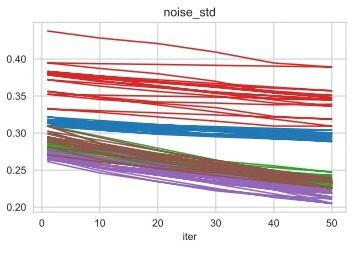
\includegraphics[width=0.5\textwidth]{imagenes/conv1_noise.jpg}
	\caption{Convergencia de noise.}
	\label{fig:conv1_noise}
\end{figure}


En el eje 'x' de cada cuadro se puede el número de iteración al que corresponde cada medida aproximada, mientras que en el eje 'y' se observa el valor del parámetro correspondiente. Los valores correspondientes a variable medida del paciente se gráfica con un color distinto en el caso de \textit{g}, \textit{v0} y \textit{noise}.Hay seis colores diferentes en cada una de estas gráfica, ya que se ha hecho el estudio para seis marcadores distintos: ABETA, HVLTRDLY, LNS, MEANCAU, SDMT y SFT. Por otra parte, cada linea representa las estimaciones de cada uno de los 10 modelos generados.\\

\subsection{Curvas características individuales}
Por otro lado, se gráfican las trayectorias \textit{'short-term'} que representan la estimación de la progresión de cada uno de los marcadores del paciente escogido.\\

El programa genera dos conjunto de seis cuadros para cada uno de los 10 modelos, siendo cada cuadro la estimación de los valores de una variable y el primer conjunto grafica los números normalizados de las mismas y el segundo en escala original. Es decir, se obtienen un total de veinte conjuntos con seis gráficas en su interior, ya que se trabaja con un bootstrap de valor 10, lo que indica que se generan 10 modelos. \\

Además de representarse en cada cuadro la curva estimada, se indican los valores de cada variable en cada observación del paciente con un punto, para así poder ver cuan precisa es la estimación de la trayectoria a corto plazo.\\

De manera ilustrativa, en este documento se muestran las gráficas dibujadas para el modelo número cinco,  viendo en primer lugar los valores normalizados para las seis variables escogidas en la imagen\ref{fig:trayM5norm} y después las curvas para los valores originales en la figura \ref{fig:trayM5orig}.\\

\begin{figure}[t]
	\centering
	\includegraphics[width=1\textwidth]{imagenes/trajectory\_norm\_plot\_model\_5.png}
	\caption{Trayectoria Normalizada del modelo 5.}
	\label{fig:trayM5norm}
\end{figure}

\begin{figure}[t]
	\centering
	\includegraphics[width=1\textwidth]{imagenes/trajectory\_orig\_plot\_model\_5.png}
	\caption{Trayectoria original del modelo 5.}
	\label{fig:trayM5orig}
\end{figure}

El resto de representaciones se pueden encontrar en la siguiente ruta del proyecto:
\begin{center}
		\texttt{Demos/rroca\_python/pred\_sujeto/\\
		plots/norm\_orig}. 
\end{center}


\section{Modelos de progresión con múltiples sujetos}
Como resultados se obtienen los parámetros correspondientes a las prestaciones de los DPMs. Con ellos se podrán comparar, entre los distintos modelos estimados,las predicciones tanto de la progresión de la enfermedad en los distintos pacientes, como el pronóstico estimado y el estado cognitivo de los mismos \cite{ghazi2021robust}. El objetivo de esto es encontrar la combinación de biomarcadores que sirva para predecir el avance de la enfermedad y pronosticar el declive cognitivo de una forma más precisa y eficaz. \\

Todas las métricas calculadas con este propósito se ubican en el directorio:
\begin{center}
	\texttt{/home/rroca/demo/multi\_leaspy/outputs/prestaciones}
\end{center}

Para cada DPM se genera una carpeta llamada \texttt{Leaspy\_vars\_} seguido de los índices de los marcadores escogidos para ese modelo (por ejemplo: \texttt{5\_10\_11}). En ellas se guardan distintos Excels para guardar los valores del MAE y NMAE para los grupos de \textit{train} y de \textit{test}. También contienen archivos .NPY con las puntuaciones de progresión de la enfermedad (DPS) para los dos conjuntos de individuos, y así poder cargar los valores desde el programa si fuera necesario. Por último también se crean dos hojas de cálculo donde se almacenará la media del MAE y del NMAE del modelo concreto y la media de área bajo la curva y los distintos tiempos de conversión y la reserva cognitiva. Esto valores, además de guardarse dentro de cada carpeta por separado, se van añadiendo a dos Excels generales, llamados \texttt{PRESTACIONES\_GENERALES\_MAE.xlsx} y \texttt{PRESTACIONES\_GENERALES\_diag.xlsx} donde cada fila recoge la media de las métricas para los modelos que se van estimando. Estos dos ficheros se ubican directamente en la carpeta:
\begin{center}
	\texttt{/home/rroca/demo/multi\_leaspy/outputs/prestaciones}
\end{center}


\subsection{Evaluación de las trayectorias estimadas}
Para comprobar la rigurosidad de las trayectorias \textit{short-term} estimadas, se implementa la estimación del NMAE. Para cada modelo, es la media de la diferencias entre las estimaciones en escala normalizada y las muestras en cada tiempo muestreado. Cada una de las variables obtiene valor de un NMAE.\\

Además, se consiguió realizar la interpolación inversa de los valores para obtener el error medio absoluto (MAE) en la escala original de cada biomarcador. Se calculó la media para el conjunto de pacientes tanto de entrenamiento como de test para cada uno de los bootstraps y para cada una de las variables de cada modelo estimado. Por ejemplo, para el modelo formado por los marcadores MOCA, LNS y SFT (con índices 1,5 y 10) se obtienen las tablas de las figuras \ref{tabla_MAE_train} y \ref{tabla_MAE_test} para el MAE de \textit{train} y de \textit{test}. \\

\begin{table}[h!]
	\centering
	\begin{tabular}{|c|c|c|c|}
		\hline
		btstrp & \textbf{moca} & \textbf{lns} & \textbf{sft} \\ \hline
		0 & 1.6582 & 1.4737 & 7.8544 \\ \hline
		1 & 1.7160 & 1.4912 & 7.3873 \\ \hline
		2 & 1.6892 & 1.5227 & 7.7018 \\ \hline
		3 & 1.6896 & 1.5120 & 7.3432 \\ \hline
		4 & 1.6656 & 1.5622 & 7.6081 \\ \hline
		5 & 1.6865 & 1.5595 & 7.5482 \\ \hline
		6 & 1.6567 & 1.5500 & 7.5810 \\ \hline
		7 & 1.6903 & 1.5761 & 7.5575 \\ \hline
		8 & 1.7050 & 1.5848 & 7.4854 \\ \hline
		9 & 1.6774 & 1.5873 & 7.5820 \\ \hline
	\end{tabular}
	\caption{MAE de los diez \textit{bootstraps} para MOCA, LNS y SFT para los pacientes de entrenamiento.}
	\label{tabla_MAE_train}
\end{table}

\begin{table}[h!]
	\centering
	\begin{tabular}{|c|c|c|c|}
		\hline
		btstrp & \textbf{moca} & \textbf{lns} & \textbf{sft} \\ \hline
		0 & 1.7401 & 1.4582 & 6.7184 \\ \hline
		1 & 1.8033 & 1.4592 & 6.3295 \\ \hline
		2 & 1.7849 & 1.4951 & 6.6530 \\ \hline
		3 & 1.7797 & 1.4815 & 6.3722 \\ \hline
		4 & 1.7444 & 1.5166 & 6.5898 \\ \hline
		5 & 1.8134 & 1.5225 & 6.6369 \\ \hline
		6 & 1.7344 & 1.4912 & 6.6888 \\ \hline
		7 & 1.7944 & 1.5486 & 6.6537 \\ \hline
		8 & 1.8161 & 1.5529 & 6.5911 \\ \hline
		9 & 1.8219 & 1.5663 & 6.6685 \\ \hline
	\end{tabular}
	\caption{MAE de los diez \textit{bootstraps} paralos biomarcadores MOCA, LNS y SFT para los pacientes de prueba.}
	\label{tabla_MAE_test}
\end{table}

Además de las tablas generadas para visualizar el MAE y el NMAE de cada modelo, se genera un Excel llamado \texttt{PRESTACIONES\_GENERALES\_MAE} donde se van añadiendo las medias del error medio absoluto y del error medio absoluto normalizado para cada modelo estimado. Esto permite comparar la precisión de la trayectoria \textit{short-term} estimada para cada uno, visualizando la tabla de la figura \ref{tab:nmae_mae_resultados}.

\begin{table}[t]
	\centering
	\begin{tabular}{|c|c|c|c|c|}
		\hline
		\textbf{\scriptsize{INDEX}} & \textbf{\scriptsize{NMAE\_train}} & \textbf{\scriptsize{NMAE\_test}} & \textbf{\scriptsize{MAE\_train}} & \textbf{\scriptsize{MAE\_test}} \\ \hline
		2\_11\_16 & 0.154 & 0.148 & 1.337 & 1.267 \\ 
		& 0.143 & 0.158 & 4.828 & 4.740 \\ 
		& 0.103 & 0.094 & 235.426 & 219.423 \\ \hline
		1\_2\_4   & 0.187 & 0.181 & 1.965 & 2.065 \\ 
		& 0.249 & 0.245 & 1.896 & 1.854 \\ 
		& 0.247 & 0.237 & 2.273 & 2.206 \\ \hline
		10\_11\_15& 0.101 & 0.101 & 4.787 & 4.455 \\ 
		& 0.141 & 0.158 & 4.965 & 4.749 \\ 
		& 0.094 & 0.094 & 133.853 & 139.667 \\ \hline
		...  & ... & ... & ... & ...\\ \hline
	\end{tabular}
	\caption{Métricas NMAE y MAE para los modelos considerados.}
	\label{tab:nmae_mae_resultados}
\end{table}




\subsection{Clasificación del estado clínico}
Para clasificar el estado cognitivo se utiliza  un clasificador bayesiano basado en el 'Disease Progresion Score'(DPS)($s_{ij}$) y que utiliza un kernel de estimación de la densidad (KDE) basado en estimaciones acordes.
\begin{equation}
	s_{ij}=\alpha_{i}t_{ij}+\beta_{i}
\end{equation}

 Para medir la fiabilidad de la probabilidad a posteriori de desarrollo del declive cognitivo se utiliza como parámetro el Área Bajo la Curva (AUC).Esto mide la precisión del modelo de determinar la aparición del deterioro cognitivo comparándolo con las etiquetas (\textit{CN} o \textit{MCI}) de los pacientes en cada una de las visitas.\\
 
 Un AUC más cercano a 1 indica que el las predicciones realizadas por el modelo son fiables. Por lo que con los resultados obtenidos se esperan encontrar valores mas cercanos a 1 que a 0,5. Para conseguir un modelo robusto, se calcula un Area Bajo la Curva para cada \textit{bootstrap} y luego se calcula la media. Este valor se guarda tanto en un archivo \texttt{.xlsx} dentro del directorio de \texttt{prestaciones} en una carpeta que indique el modelo evaluado, como en el excel general donde se van guardando todas las metricas, el cual se encuentra en el directorio:

 \begin{center}
 	\texttt{/home/rroca/demo/multi\_leaspy/outputs/prestaciones
 		/PRESTACIONES\_GENERAL\_diag.xlsx}
 \end{center}

Otro indicador de la exactitud de los modelo son los parámetros \textbf{percentage\_PD\_CU} y \textbf{percentage\_PD\_MCI}. Estos se encuentran en el archivo del directorio:
\begin{center}
	\texttt{/home/rroca/demo/multi\_leaspy/outputs/prestaciones
		/PRESTACIONES\_GENERAL\_diag.xlsx}
\end{center}
en las columnas con los mismos nombres y con el indicador de diferenciación del grupo de \textit{train} y de \textit{test}. \\

Estas métricas miden el rendimiento de los modelos para predecir el inicio dela conversión a deterioro cognitivo leve (MCI) a partir de los datos de los sujetos. Por un lado mide el porcentaje de pacientes que predice correctamente como convertidos a MCI y lo guarda en las columnas \textbf{perc\_PD\_MCI\_test} y \textbf{perc\_PD\_MCI\_train}. Por otro lado, se calcula el porcentaje de sujetos que el modelo predice correctamente como sanos (CU) y los registra en las columnas con nombre \textbf{perc\_PD\_CU\_test} y \textbf{perc\_PD\_CU\_train}. 




\subsection{Medidas relacionadas con los plazos de conversión hacia el declive cognitivo}

Por último, se calculan las correlaciones de los tiempos de conversión hacia el declive cognitivo de los individuos de entrenamiento y de prueba, y también de la reserva cognitiva de ambos grupos. Estos medidores indican, por un lado la precisión a la hora de predecir a que edad convierten los pacientes, y por otro lado la exactitud del cálculo de años de reserva que les quedan antes de entrar en la fase de deterioro cognitivo. \\

Se calculan estos dos parámetros ya que no es lo mismo comparar las edades estimadas, que los años de reserva. En el primer caso como la escala es mucho mayor aunque el modelo tenga un error a la hora de predecir de un par de años, la correlación variaría en unas décimas. Mientras que en el caso de la reserva cognitiva, una diferencia de dos años puede suponer un que el índice pase de un 0,7 de precisión a un 0,2. Por lo que los parámetros de la reserva cognitiva nos da un valor más exacto de cuan fiable es el modelo.\\

Estas medidas, al igual que la del Área Bajo la Curva (AUC) se guardan en el excel del directorio:

\begin{center}
	\texttt{/home/rroca/demo/multi\_leaspy/outputs/prestaciones
		/PRESTACIONES\_GENERAL\_diag.xlsx}
\end{center}

Más concretamente en las cuatro columnas con los siguientes nombres:
\begin{itemize}
	\item \textbf{corr\_PD\_MCI\_reserve\_train} y \textbf{corr\_PD\_MCI\_reserve\_test}: medidas de la correlación entre la reserva cognitiva real y la estimada para \textit{train} y \textit{test}
	\item \textbf{corr\_PD\_MCI\_age\_train} y \textbf{corr\_PD\_MCI\_age\_test}: parámetrso para la correlación entre las edades de conversión reales y las estimadas para los individuos de entrenamientos y de prueba.
\end{itemize}

En la figura \ref{tab:resultados_biomarcadores} se muestran las medidas de algunos de los modelos estimados y guardados en el fichero \texttt{PRESTACIONES\_GENERAL\_diag.xlsx}. Para referirse a la medidas tomadas para el grupo de entrenamiento se adjunta un 1 al final del nombre de las columnas, y para referirse al grupo de prueba se adjunta un 2.


\begin{table}[H]
	\centering
	\begin{adjustbox}{max width=\textwidth}
		\begin{tabular}{|c|c|c|c|c|c|c|c|c|c|c|}
			\hline
			\rotatebox{90}{\scriptsize{\textbf{INDEX}}} & \rotatebox{90}{\scriptsize{\textbf{AUC\_1}}} & \rotatebox{90}{\scriptsize{\textbf{AUC\_2}}} & \rotatebox{90}{\scriptsize{\textbf{perc\_PD\_CU\_2}}} & \rotatebox{90}{\scriptsize{\textbf{perc\_PD\_MCI\_2}}} & \rotatebox{90}{\scriptsize{\textbf{corr\_PD\_MCI\_age\_2}}} & \rotatebox{90}{\scriptsize{\textbf{corr\_PD\_MCI\_reserve\_2}}} & \rotatebox{90}{\scriptsize{\textbf{perc\_PD\_CU\_1}}} & \rotatebox{90}{\scriptsize{\textbf{perc\_PD\_MCI\_1}}} & \rotatebox{90}{\scriptsize{\textbf{corr\_PD\_MCI\_age\_1}}} & \rotatebox{90}{\scriptsize{\textbf{corr\_PD\_MCI\_reserve\_1}}} \\ \hline
			1\_5\_14       & 0.797 & 0.800 & 94.737 & 26.087 & 0.979 & 0.011 & 98.971 & 25.789 & 0.970 & 0.505 \\ \hline
			4\_5\_14\_16   & 0.738 & 0.787 & 98.246 & 14.783 & 0.932 & 0.389 & 98.025 & 16.316 & 0.968 & 0.420 \\ \hline
			1\_5\_10\_18   & 0.789 & 0.796 & 95.088 & 16.522 & 0.960 & 0.489 & 98.683 & 22.237 & 0.983 & 0.579 \\ \hline
			5\_10\_11\_14  & 0.786 & 0.824 & 96.140 & 27.391 & 0.957 & 0.504 & 96.831 & 25.658 & 0.973 & 0.356 \\ \hline
			...  & ... & ... & ... & ... & ... & ... & ... & ... & ... & ... \\ \hline
		\end{tabular}
	\end{adjustbox}
	\caption{Métricas de evaluación clínica para diferentes modelos.}
	\label{tab:resultados_biomarcadores}
\end{table}


\section{Análisis masivo: \textit{multi\_Leaspy} y\textit{ multi\_RPDPM}}
Una vez obtenidas las medidas de distintos conjuntos de biomarcadores, se comparan entre los dos métodos de predicción utilizados: Leaspy y RPDPM. Cabe destacar la preferencia de vectores de menor dimensión, ya que implicarían un menor número de observaciones y de medidas a tomar en los pacientes para poder predecir el avance de la enfermedad, y por lo tanto un menor coste. \\

Para comparar la precisión de los distintos modelos, se tomó como medida de referencia la multiplicación de la detección de pacientes cognitivamente normales (\textbf{perc\_PD\_CU}) por la correlación con la reserva cognitiva (\textbf{corr\_PD\_MCI\_reserve}). En las tablas \ref{tab:RPDPM3} y \ref{tab:RPDPM4y5} se muestran los resultados de los vectores de características que mejores puntuaciones han mostrado para el método RPDPM en las medidas de detección de sujetos cognitivamente normales y con declive cognitivo leve, y en las correlaciones de la edad y de la reserva cognitiva. En el primer caso se muestran vectores de menor dimensión, mejores para aplicaciones clínicas ya que solo haría falta observar tres biomarcadores, y en el segundo caso para combinaciones de mayor tamaño. En las tablas \ref{tab:LEASPY3} y \ref{tab:LEASPY4y5} se muestran los vectores con mejores resultados para el caso de Leaspy, dividiendo las tablas también en función del numero de características de las combinaciones.

A continuación, se muestran los vectores de marcadores que mejores resultados han dado tanto en Leaspy como en RPDPM, en función de la cantidad de variables utilizadas. 

\subsection{Leaspy}
Para el método de Leaspy, el vector de menor dimensión que mejores resultados a mostrado es el formado por los biomarcadores:
\begin{center}
	\textbf{\{updrs\_totscore, tau y asyn\}}
\end{center}
En cuanto a los vectores de dimensiones mayores (cuatro o cinco biomarcadores), que mejores resultados han dado en las métricas de calidad de detección del estado de los pacientes y de la aparición del declive cognitivo son los siguientes:
\begin{center}
	\textbf{\{updrs3\_score\_on, updrs\_totscore\_on, ptau, asyn\}}		
\end{center}
\begin{center}
	\textbf{\{updrs3\_score\_on, updrs2\_score, ptau, mean\_caudate, mean\_putamen\}}
\end{center}

Estos tres vectores muestran las siguientes puntuaciones en las medidas de detección de pacientes PD\_CU en el grupo de \textit{test}: 100, 98.24 y 97.36. Y sus valores en la correlación con la reserva cognitiva es 1 en los tres casos. \\

Dado que los valores son prácticamente iguales para las tres combinaciones, el más  conveniente para la práctica clínica es el de menor dimensión como ya se explicó previamente. \\

\subsection{RPDPM}
Para el caso de RPDPM desarrollado en MATLAB, los vectores que mejores resultados mostraron con dimensiones de 5, 4 y 3 biomarcadores fueron:

\begin{center}
	\textbf{\{GDS, UPSIT, REM, LNS, ADL\}}		
\end{center}
\begin{center}
	\textbf{\{UPSIT, LNS, SDMT, ADL\}}
\end{center}
\begin{center}
	\textbf{\{SDMT, JLO, HVLTRDLY\}}
\end{center}

De estos tres, el que mejores puntuaciones muestra es al mismo tiempo el de menor dimensión, por lo que la combinación de biomarcadores formada por SDMT, JLO y HVLTRDLY también es el más apropiado para la aplicación clínica. Los valores de estos tres vectores en cuanto a la detección de pacientes PD\_CU son respectivamente: 97.75, 97.46 y 98.92. Y los valores de la correlación de la reserva cognitiva para los pacientes de test para esas combinaciones son: 0.432, 0.654 y 0.725.\\

\begin{table}[H]
	\centering
	\begin{adjustbox}{max width=\textwidth}
		\begin{tabular}{|c|c|c|c|c|c|}
			\hline
			\textbf{BIOMARCADORES} & \textbf{\%PD\_CU} & \textbf{\%PD\_MCI} & \textbf{corr\_PD\_MCI\_edad} & \textbf{corr\_PD\_MCI\_reserva} & \textbf{AUC} \\ \hline
			U, L, S, A  & 97.46 & 32.47 & 0.978 & 0.654 & 0.803 \\ \hline
			U, L, S, M  & 97.33 & 28.52 & 0.968 & 0.551 & 0.790 \\ \hline
			S, J, H, M & 98.75 & 30 & 0.973 & 0.684 & 0.794 \\ \hline
			G, L, S, A  & 97.58 & 36.67 & 0.980 & 0.613 & 0.813 \\ \hline
			G, U, R, L, A & 97.75 & 39.63 & 0.982 & 0.432 & 0.833 \\ \hline
		\end{tabular}
	\end{adjustbox}
	\caption{Mejores combinaciones de biomarcadores de mayor dimensión con 4 o 5 características para el método de RPDPM, basado en las medidas de la detección de PD\_CU (\%PD\_CU), detección de PD\_MCI (\%PD\_MCI), correlación con la edad (corr\_PD\_MCI\_edad), correlación con la reserva (corr\_PD\_MCI\_reserva) y Área Bajo la Curva (AUC). U=UPSIT, L=LNS, S=SDMT, A=ADL, M=MEANPUT, J=JLO, H=HVLTRDLY, G=GDS, R=REM.}
	\label{tab:RPDPM4y5}
\end{table}

\begin{table}[H]
	\centering
	\begin{adjustbox}{max width=\textwidth}
		\begin{tabular}{|c|c|c|c|c|c|}
			\hline
			\textbf{BIOMARCADORES} & \textbf{\%PD\_CU} & \textbf{\%PD\_MCI} & \textbf{corr\_PD\_MCI\_edad} & \textbf{corr\_PD\_MCI\_reserva} & \textbf{AUC} \\ \hline
			S, J, H  & 98.92 & 29.75 & 0.977 & 0.726 & 0.795 \\ \hline
			L, S, A & 96.63 & 36.05 & 0.975 & 0.584 & 0.795 \\
			\hline
			G, L, J & 98.46 & 36.91 & 0.986 & 0.564 & 0.820 \\
			\hline
			G, L, S & 97.21 & 38.64 & 0.980 & 0.520 & 0.803 \\ \hline
			J, H, SF & 98.92 & 28.77 & 0.982 & 0.564 & 0.817 \\   \hline
		\end{tabular}
	\end{adjustbox}
	\caption{Mejores combinaciones de biomarcadores de menor dimensión con 3 características para el método de RPDPM, basado en las medidas de la detección de PD\_CU (\%PD\_CU), detección de PD\_MCI (\%PD\_MCI), correlación con la edad (corr\_PD\_MCI\_edad), correlación con la reserva (corr\_PD\_MCI\_reserva) y Área Bajo la Curva (AUC). S=SDMT, J=JLO, H=HVLTRDLY, L=LNS, A=ADL, G=GDS, SF=SFT.}
	\label{tab:RPDPM3}
\end{table}


\begin{table}[H]
	\centering
	\begin{adjustbox}{max width=\textwidth}
		\begin{tabular}{|c|c|c|c|c|c|}
			\hline
			\textbf{BIOMARCADORES} & \textbf{\%PD\_CU} & \textbf{\%PD\_MCI} & \textbf{corr\_PD\_MCI\_edad} & \textbf{corr\_PD\_MCI\_reserva} & \textbf{AUC} \\ \hline
			 U3O, UTO, P, A & 98.25 & 1.74 & 1.00 & 1.00 & 0.696\\ \hline
			 SC, M, B, S & 100 & 12.17 & 0.997 & 0.881 & 0.815\\ \hline
			 U3O, U3, U2, UTO & 98.60 & 6.52 & 0.996 & 0.908 & 0.730 \\ \hline
			 U3O, U2, P, MC, MP  & 97.37 & 3.48 & 1.00 & 1.00 & 0.769\\ \hline
			 SC, M, SF, HI, R & 98.77 & 8.69 & 1.00 & 1.00 & 0.811\\ \hline
		\end{tabular}
	\end{adjustbox}	
	\caption{Mejores combinaciones de biomarcadores de mayor dimensión con 4 o 5 características para el método de Leaspy, basado en las medidas de la detección de PD\_CU (\%PD\_CU), detección de PD\_MCI (\%PD\_MCI), correlación con la edad (corr\_PD\_MCI\_edad), correlación con la reserva (corr\_PD\_MCI\_reserva) y Área Bajo la Curva (AUC). U3O=UPDRS3\_SCORE\_ON, UTO=UPDRS\_TOTSCORE\_ON, P=PTAU, A=ASYN, SC=SCOPA, M=MSEADLG, B=BJLOT, S=SDMT, U3=UPDRS3\_SCORE, U2=UPDRS2\_SCORE, MC=MEAN\_CAUDATE, MP=MEAN\_PUTAMEN, SF=SFT, HI=HVLT\_INMEDIATERECALL, R=REM.}
	\label{tab:LEASPY4y5}
\end{table}



\begin{table}[H]
	\centering
	\begin{adjustbox}{max width=\textwidth}
		\begin{tabular}{|c|c|c|c|c|c|}
			\hline
			\textbf{BIOMARCADORES} & \textbf{\%PD\_CU} & \textbf{\%PD\_MCI} & \textbf{corr\_age\_MCI} & \textbf{corr\_reserve\_MCI} & \textbf{AUC} \\ \hline
			UT, T, A & 100 & 6.96 & 1.00 & 1.00 & 0.723 \\ \hline
			UTO, T, A & 99.83 & 10.00 & 0.970 & 0.927 & 0.725 \\ \hline
			UTO, P, A & 99.83 & 8.26 & 1.00 & 1.00 & 0.724 \\ \hline
			U2, UTO, AB & 100 & 3.48 & 1.00 & 1.00 & 0.718 \\ \hline
			SC, H, R & 100 & 6.52 & 1.00 & 1.00 & 0.74 \\ \hline
		\end{tabular}
	\end{adjustbox}
	\caption{Mejores combinaciones de biomarcadores de menor dimensión con 3 características, basadas en las medidas de la detección de PD\_CU (\%PD\_CU), detección de PD\_MCI (\%PD\_MCI), correlación con la edad (corr\_age\_MCI), correlación con la reserva (corr\_reserve\_MCI) y Área Bajo la Curva (AUC). UT=UPDRS\_TOTSCORE, T=TAU, A=ASYN, UTO=UPDRS\_TOTSCORE\_ON, P=PTAU, U2=UPDRS2\_SCORE, AB=ABETA, SC=SCOPA, H=HVLTRDLY, R=REM.}
	\label{tab:LEASPY3}
\end{table}



\chapter{Discusiones} \label{discusiones}

\section{Estudio transversal sobre la influencia de marcadores en el declive cognitivo en la Enfermedad de Parkinson}
Los resultados del análisis en Python revelan la influencia de las variables estudiadas en el deterioro cognitivo de pacientes con Enfermedad de Parkinson.\\

Observando las dos tablas resultantes, se puede llevar a algunas conclusiones sobre los distintos parámetros. En la tabla \ref{tab:tabla3}, tras la comparación de los valores en la linea de base, se observan diferencias relevantes en algunas filas entre el grupo de pacientes con Parkinson y el grupo de control. En primer lugar, cabe destacar que para que el estudio sea fiable, ambos grupos tiene las mismas características demográficas. Sin embargo, entre los parámetros cognitivos y clínicos se encuentran varios marcadores con indicador de significancia en la columna del Post-hoc. Entre los que se pueden señalar están GDS, REM, MOCA, SDMT y MEANPUT. \\

Por otra parte, en la tabla \ref{tab:tabla2} destaca la relación entre las distintas características de estudio y el desarrollo de diferentes niveles de declive cognitivo en los pacientes PD. Los valores de p-valor y los indicadores de post-hoc señalan que variables pueden tener un efecto significativo en el transcurso del deterioro cognitivo en los distintos subgrupos. Entre ellas, diferenciadas por tener un \textit{valor p} igual o por debajo de 0.001, se ve como por ejemplo el SDMT y el MEANCAU son considerables tanto en la comparación entre sujetos cognitivamente normales y con deterioro cognitivo como entre cognitivamente normales y los pacientes que desarrollaron demencia. Sin embargo, hay factores que solo muestran efectos significativos en una de las dos comparativas, marcados con un solo indicador (\textit{a} o \textit{b}). Entre estos últimos se encuentran REM, con diferencias importantes solo entre PD\_CU y PD\_MCI; o A$\beta_{42}$, con diferencia notable entre PD\_CU y PDD. En esta tabla, dentro de las variables demográficas, la edad es un indicador del avance de los pacientes hacia un deterioro cognitivo medio y de la aparición de la demencia. Además, se puede ver como las variables cognitivas tienen una gran importancia en el desarrollo del declive cognitivo, sobre todo indicando la evolución de PD\_CU a PD\_MCI. Aún así, los parámetros LNS, SDMT, INMEDIATE y SFT también marcan la evolución de los sujetos hacia el grupo con demencia. Entre las variables clínicas, ABETA y PTAU señalan la evolución hacia el colectivo PDD, y MEANCAU es una característica significativa tanto de la aparición del deterioro cognitivo como de la demencia. \\

Es importante destacar las variables que resultaron significativas en el análisis, tanto en la tabla \ref{tab:tabla3} como en la tabla \ref{tab:tabla2}. Todas ellas son medidas cognitivas y clínicas. Entre estas, se encuentran: UPSIT, SDMT, INMEDIATE, SFT y MEANCAU. Estos parámetros pueden tener implicaciones cruciales para el diagnostico anticipado y el desarrollo de estrategias para el tratamiento.\\

En resumen, en los resultados de este estudio destacan marcadores significativos en el declive cognitivo en la Enfermedad de Parkinson. Estos hallazgos tienen el potencial de mejorar la predicción temprana de la enfermedad y permitir intervenciones más efectivas. La identificación de estos marcadores puede conducir a un enfoque más personalizado en el tratamiento de pacientes con Parkinson, mejorando así su calidad de vida y ofreciendo esperanza a quienes se ven afectados por esta enfermedad. También es importante tener en cuenta que los resultados obtenidos pueden variar según la población y otros factores.


\section{Análisis longitudinal y reconstrucción temporal de un único sujeto}

En las gráficas que podemos ver en las figuras \ref{fig:conv1_gvsource}, \ref{fig:conv1_tauxi} y \ref{fig:conv1_noise} se demuestra la convergencia de los parámetros estimados por Leaspy a lo largo de 50 iteraciones, indicando la validez de los parámetros (g, v0, sources, tau, xi, noise).\\

En el caso de las gráficas obtenidas que estiman las trayectorias \textit{'short-term'} de cada variable, se puede observar en la figura \ref{fig:trayM5norm} como en los parámetros ABETA, MEANCAU Y HVLTRDLY su estimación no se cruza con la curva de unión de los puntos de sus observaciones. En las otras tres (SDMT, LNS, SFT) si que se puede ver una clara intersección entre las rectas, ya que a mayor numero de mediciones mas precisa es la estimación.


\section{Modelos de progresión con múltiples sujetos}
Comparando de forma general los dos métodos de modelado utilizados en este trabajo, a pesar de que Leaspy obtiene resultados robustos para la predicción de enfermedades como el Alzheimer, muestra ciertas variaciones para el caso del Parkinson. Además, en la mayoría de las métricas evaluadas, RPDPM (\textit{Robust Parametric Disease Progression Modeling}) tiene un rendimiento superior para el conjunto de todos los modelos estimados.\\

Para el caso de la detección de pacientes PD\_CU (cognitivamente normales) en el grupo de \textit{test}, se detectan valores similares para ambos métodos, siendo ligeramente superiores para RPDPM, sobre un 0,1\% mayores que los de Leaspy. Para el caso de la detección de sujetos PD\_MCI (deterioro cognitivo leve), hay una diferencia mayor, siendo entorno a un 20\% más exacto utilizando RPDPM. En la correlación con la reserva cognitiva Leaspy da una media superior a RPDPM, sobre un 2\% por encima, mientras que en el Área Bajo la Curva (AUC), RPDPM vuelve a mostrar valores superiores a Leaspy, siendo un 5\% más preciso.\\

Centrando la discusión en la aplicación clínica, para el caso de RPDPM \cite{ghazi2021robust} los valores son bastante similares para los vectores de menor dimensión formados por tres biomarcadores y para los de mayor dimensión, compuestos por cuatro o cinco características. La variación en todas las prestaciones es menor del 0,3\%. En el caso de Leaspy, hay una diferencia más grande entre los vectores de mayor y menor dimensión, obteniendo mejores resultados en el caso de los de tamaño mayor. Esto indica por un lado, la posibilidad de utilizar el método de RPDPM tomando un menor número de muestras en los pacientes, ya que harían falta observaciones de un menor número de marcadores para obtener resultados precisos. En el caso de Leaspy, las predicciones llevadas a cabo con un menor numero de características son menos precisas que las que emplean más marcadores para el mismo método. También muestran peores resultados que los obtenidos para el mismo número de biomarcadores con el método RPDPM. En definitva, para obtener resultados óptimos con Leaspy, es preferible utilizar un conjunto de características más amplio. A diferencia de RPDPM, donde la reducción en la cantidad de biomarcadores no afecta significativamente la precisión, Leaspy parece depender en mayor medida de un conjunto más completo de datos para mantener su robustez en las predicciones. \\

La combinación de características que mejores resultados ha dado para los modelos generados en RPDPM es upsit, LNS, SDMT y ADL y para Leaspy es updrs\_totscore, tau y asyn. Los valores del porcentaje de pacientes pCU detectados son respectivamente 97.46\% y 100\%, el porcentaje de pacientes pMCI es 32.47\% y 6.96\%, y la correlación con la reserva 65.41\% y 100\% para cada caso. En los valores medios de todas las combinaciones generadas, se ha visto que Leaspy muestra porcentajes más bajos. No obstante, en estos valores se refleja como, a excepción de la medida de la detección de pacientes con deterioro cognitivo leve,  en los otros dos parámetros, Leaspy muestra valores más altos. Esto refleja una mayor variabilidad en las predicciones de los modelos evaluados con Leaspy.\\

Por otro lado, el vector de RPDPM formado por los tres biomarcadores sdmt, bjlot y hvltrdly da mejores resultados que la combinación de mayor dimensión para el caso del conjunto de pacientes de prueba, siendo un factor positivo para la aplicación clínica de este método. 

En cuanto al desplazamiento espacial de las trayectorias pronosticadas, medido a través del Error Absoluto Medio (MAE), se observa como para aquellos modelos en los que se obtuvieron los mejores resultados de diagnóstico clínico, también muestran valores mas bajos en el MAE de los biomarcadores característicos. Esto indica una mayor precisión en la predicción y estimación de las curvas de evolución de la enfermedad, lo cual sucede tanto para RPDPM como para Leaspy.




\chapter{Conclusiones}

Se presentan a continuación las conclusiones del estudio realizado en este trabajo y una propuesta de futuras tareas para su continuación y mejora. 


\section{Conclusión}

Este trabajo se centró en la predicción del deterioro cognitivo en pacientes con enfermedad de Parkinson utilizando Leaspy, una herramienta de software desarrollada para estimar el avance de enfermedades neurodegenerativas. A lo largo de este estudio, se analizaron los datos longitudinales de una cohorte de 423 pacientes, con el objetivo de evaluar la efectividad de los modelos de progresión de la enfermedad (DPMs) estimados mediante este entorno.\\

En cuanto a la identificación de biomarcadores que influyen en la aparición del declive cognitivo, se consiguieron resultados prometedores. El análisis realizado con los datos de los pacientes al inicio del estudio, reveló que marcadores como el SDMT y el MEANCAU son significativos en la progresión de la enfermedad. Tanto en el avance desde un estado cognitivamente normal (CU) hasta uno de deterioro cognitivo leve (MCI), como en la evolución hacia la demencia. Estos resultados concuerdan con los de la bibliografía existente y sirven para indicar la importancia de estos marcadores en el seguimiento clínico de los pacientes.\\

Para evaluar la predicción de la progresión de la enfermedad, se desarrolló un algoritmo utilizando Leaspy que permitió estimar la trayectoria de la enfermedad, tanto para un único paciente como para toda la cohorte de 423 individuos. Las curvas estimadas para los pacientes individuales mostraron una buena concordancia con las observaciones tomadas, lo que sugiere que Leaspy tiene el potencial de ser una herramienta útil para la predicción personalizada de la evolución del Parkinson en sujetos nuevos. Sin embargo, al aplicar el modelos al conjunto completo de pacientes, se observaron algunas limitaciones, particularmente en la precisión de la detección de sujetos con deterioro cognitivo leve. Estos resultados indican que, aunque Leaspy puede ofrecer predicciones robustas en ciertos contextos, su rendimiento es variable y puede depender en gran medida de la selección y el número de biomarcadores utilizados.\\

La comparación con el método RPDPM (\textit{Robust Parametric Disease Progression Modeling}) indicó que, aunque Leaspy muestra ventajas en algunos aspectos como la detección de sujetos congitivamente normales y la correlación con la reserva cognitiva, el RPDPM fue en general más preciso detectando pacientes MCI y en la estimación del AUC. En conclusión, RPDPM es un método más adecuado para el pronóstico del avance de la enfermedad de Parkinson y para la predicción de su evolución, puesto que mantiene su precisión empleando un bajo número de marcadores observados, siendo beneficioso para su aplicación clínica.\\


\section{Desarrollos futuros}

Tras las conclusiones obtenidas, se sugieren posibles desarrollos a llevar a cabo en un futuro. En primer lugar, se deberían generar modelos con combinaciones de biomarcadores distintas y con vectores de mayor y de menor tamaño a los generados en este trabajo. El objetivo sería encontrar una combinación de características que muestre mejores resultados que las obtenidas hasta el momento. \\

Además, sería relevante la comparación de los métodos utilizados (Leaspy y RPDPM) con otros modelos de progresión de la enfermedad aplicándolo a la aparición del deterioro cognitivo en el Parkinson. \\

También se podría considerar la aplicación de los modelos generados a otras cohortes de pacientes, más allá de los datos disponibles en la PPMI, para evaluar la generalización de los resultados y la robustez de las predicciones en diferentes poblaciones.\\

Por último, otro posible desarrollo a llevar a cabo sería la implementación de estos modelos en una plataforma de software clínico. Esto implicaría el desarrollo de interfaces de usuario intuitivas y la integración con sistemas de historia clínica electrónica, permitiendo a los médicos utilizar estas herramientas predictivas en tiempo real para el seguimiento y tratamiento de pacientes con Parkinson.

\appendix

\chapter{Inferencia estadística. Anova y Chi-cuadrado}

La inferencia estadística es una técnica que obtiene, a partir de una muestra, suposiciones sobre la población. Para ello utiliza distintas pruebas de hipótesis y otros métodos estadísticos, entre las que se encuentran la prueba t, Chi-cuadrado o el análisis de varianza, utilizados para encontrar distinciones entre grupos \cite{INFERENC93:online}.  \\

Su procedimiento se basa, teniendo una hipótesis sobre cierta población, en utilizar múltiples herramientas sobre una muestra para saber si la afirmación es valida o no. Para entender esto bien, primero hay que aclarar algunos conceptos previos.\\

Teniendo ya una muestra seleccionada, existen dos hipótesis opuestas a la hora de llevar a cabo el estudio. Estas se rechazarán o aceptarán en función del resultado del estudio de los datos seleccionados: 

\begin{itemize}
	\item Hipótesis nula (H0): Suposición que indica que una característica no es diferente entre grupos. Con el transcurso de la investigación se pretende demostrar que no es cierta. Por ejemplo, podría ser que dos variables no estén relacionadas.
	\item Hipótesis alternativa (H1): es lo contrario a la hipótesis nula. Es la conclusión que el investigador intenta afirmar tras su estudio e indica que sí habría una diferencia entre los grupos. En este caso sería que las variable si fueran dependientes entre si.
\end{itemize}

Para decidir si se rechaza o mantiene H0 se lleva a cabo una prueba de hipótesis. Esta está formada por técnicas estadísticas que prueban la suposición inicial con los datos seleccionados. Con este procedimiento se comprueba si no hay diferencia o relación. \\

En este proceso siempre existe un porcentaje de error, denominado nivel de significación o $\alpha$, el cual suele estar en torno al 5\%. Este factor indica la probabilidad de rechazar la hipótesis nula y que en verdad sea cierta. Esto es debido a la realización del estudio a partir de una muestra, la cual puede o no asemejarse a la población. El peor caso sucedería cuando los individuos seleccionados se desvían mucho de la norma, lo que llevaría a obtener una conclusión errónea.\\

Otro término importante es el valor \textit{p}, el cual se utiliza para decidir si rechazar la hipótesis nula. Cuando el valor p esté por encima del nivel de significación, se mantendrá, mientras que cuando este por debajo podremos rechazarla y aceptar la hipótesis alternativa \cite{ValorpSi12:online}.\\

Entre las pruebas de análisis, algunas de las más destacadas son el Análisis de Varianza (ANOVA) y el método Chi-cuadrado. En función del tipo de variables estudiadas se usaran una u otra. Estos factores se pueden clasificar en:
\begin{itemize}
	\item Variable cuantitativa: Se pueden medir numéricamente, como las cantidades. Se estudian en ANOVA.
	\item Variable cualitativa: Aquellas que no son medibles, como características o categorías. Son analizadas en pruebas como Chi-cuadrado.
\end{itemize}

\section{Anova}

El Análisis de la Varianza (ANOVA) es una técnica estadística utilizada para comprobar si hay una diferencia significativa entre la media de distintos grupos. Con ella se mide el comportamiento de una variable dependiente en función de otra independiente. Como por ejemplo, se puede medir la influencia de varios medicamentos en los niveles de azúcar de diferentes grupos. \cite{INFERENC93:online} \\

Con este método se estudia la prueba F, la cual mide el ratio entre la varianza de las medias de los grupos y el promedio de la varianza dentro de los mismos. Además, sigue una distribución conocida como "F de Fisher-Snedecor”

\begin{center}
	$F = \frac{Variaci\acute{o}n\quad entre\quad las\quad medias\quad de\quad las\quad muestras}{Variaci\acute{o}n\quad dentro\quad de\quad las\quad muestras}$
\end{center}

Siendo la siguiente ecuación la fórmula de la varianza:
\begin{center}
	$\sigma^{2} = \frac{\sum_{1}^{N} (x_{i}-\bar{X})^{2}}{N}$
\end{center}

Al cumplirse la hipótesis nula, el $F_{ratio}$  es igual a 1. Este valor aumentará al incrementar la diferencia entre las medias de los grupos. Como consecuencia, la probabilidad de que la distribución adquiera valores extremos sera menor, y también será más pequeño el \textit{p-valor}. \\

Con esta herramienta se mide la relación entre la varianza dentro de los grupos y la varianza entre grupos. Se concluye una mayor probabilidad de que existan diferencias significativas si la varianza dentro de los conjuntos es menor que entre ellos. Este resultado se muestra en la prueba F, siendo mayor al existir distinciones significativas, implicando que la hipótesis nula no es compatible.\\

Entre los conceptos de los que es necesario aclarar su significado se encuentran: 
\begin{itemize}
	
	\item Variable dependiente: elemento medido y que se ve afectado por la o las variables independientes.
	\item Variable independiente: elemento que pueden ser uno o mas y que afectan a la variable dependiente.
\end{itemize}

Además, la variable independientes, también llamadas factores, pueden tener diferentes valores, denominados niveles. En función de la cantidad de variables independientes se llevará a cabo un proceso distinto.

\subsubsection{Análisis simple de la varianza}
Este tipo de análisis, también llamado 'One-Way ANOVA', se utiliza para la comparación de la media de dos grupos con una sola variable independiente. Se estudia si existen diferencias significativas entre las medias de una variable aleatoria y los diferentes niveles de un factor. Este método es conveniente para los casos en los que el factor tiene dos o más niveles, ya que así se puede determinar si los diferentes niveles tienen un efecto significativo sobre el valor de la variable dependiente.\\

Para definir las hipótesis en un ANOVA de un factor, consideramos $\mu$ como la media de todas las observaciones sin tener en cuenta los niveles, y $\alpha_{i}$ el efecto introducido por el nivel \textit{i}. La media de cada nivel y las distintas hipótesis serán: 
\begin{center}
	Media: $\mu_{i} = \mu + \alpha_{i} $

$H_{0}$: El efecto de los niveles es nulo $(\mu_{1} = \mu_{2} = \mu_{k} = \mu)$\\
$H_{1}$: Mínimo una media se desplaza debido a un nivel $(\alpha_{i} \neq 0)$
\end{center}

Para obtener una conclusión sobre si rechazar o no la hipótesis nula, es necesario comparar las medias de la variación entre diferentes niveles con la medida de la variación dentro de cada nivel. Si el primer valor es significativamente mayor que el segundo, se podrá rechazar la hipótesis nula. Esto indicará la influencia del factor sobre la variable dependiente \cite{terradez2003analisis}.\\

Para detectar la diferencia entre medias, se estudia la varianza total, la cual se obtiene dividiendo las distintas sumas de cuadrados entre los respectivos grados de libertad. Estos valores también son denominados cuadrados medios, cuyo análisis forma parte de la técnica ANOVA. A continuación se muestran el debido desarrollo:
\begin{center}
$Variabilidad\quad total = (varianza\quad entre\quad niveles) + (varianza\quad dentro \quad de\quad los\quad niveles) = \hat{S}_{t}^{2} + \hat{S}_{E}^{2} = \hat{S}_{T}^{2}$
\end{center}

Siendo:
\begin{itemize}
	\item $\hat{S}_{t}^{2}$ (Cuadrados Medios del Factor): calcula la varianza entre las medias de los distintos niveles (Intervarianza). Divide la suma de cuadrados del factor (SST) entre los grados de libertad.
	\begin{center}
		$\hat{S}_{t}^{2} = \frac{SST}{k-1}$
	\end{center}
	\item $\hat{S}_{E}^{2}$ (Cuadrados Medios del Error): calcula la varianza dentro de los niveles (Intravarianza). Divide la suma de cuadrados residual/error (SSE) entre los grados de libertad.
	\begin{center}
		$\hat{S}_{E}^{2} = \frac{SSE}{N-k}$
	\end{center}
	\item $\hat{S}_{T}^{2}$ (Cuadrados Medios Totales): calcula la varianza muestral total (Cuasivarianza total). Divide la Suma de Cuadrados Total (TSS) entre los grados de libertad.
	\begin{center}
		$\hat{S}_{T}^{2} = \frac{TSS}{N-1}$
	\end{center}
	
	
	Sabiendo esto, el ratio de la prueba nos queda de la siguiente forma:
	\begin{center}
	$F_{ratio}=\frac{Cuadrados\quad Medios\quad del\quad Factor}{Cuadrados\quad Medios\quad del\quad Error}=\frac{\hat{S}_{t}^{2}}{\hat{S}_{E}^{2}}=\frac{intervarianza}{intravarianza}$
	\end{center}
\end{itemize}




\subsubsection{Análisis doble de la varianza}
Cuando interviene más de un factor se utiliza el 'Two-Way ANOVA'. Con este método se mide la influencia de cada uno de ellos y de sus distintos niveles sobre el elemento a medir. Para poder rechazar la hipótesis nula, que en este caso afirma que la variable dependiente no depende de la independiente, es necesario contrastarla con cada factor.\\	


En función de si el modelo tiene o no interacción, es decir, de si influye el efecto que tienen los distintos factores entre ellos, la variación total de los datos se medirá de forma distinta:

\begin{itemize}
	\item Con interacción:\\
	(Variación total en los datos) = (Variación debida al primer factor) + (Variación debida al
	segundo factor) + (Variación debida a la interacción entre factores) + (Variación debida al
	error aleatorio) 
	\item Sin interacción:\\
	(Variación total en los datos) = (Variación debida al primer factor) + (Variación debida al
	segundo factor) + (Variación debida al error aleatorio) 
\end{itemize}

\section{Chi-cuadrado}
Esta prueba de hipótesis se utiliza para saber si las diferencias de un factor cualitativo, como el género o los años de estudio, entre distintos grupos son significativas. También sirve para identificar si dos de ellos están o no relacionados, o por el contrario, si son independientes.\\

Para ello, se compara la frecuencia observada con la esperada en la muestra y se concluye si la desviación es significativa.\\

El método Chi-cuadrado tiene las siguientes aplicaciones:
\begin{itemize}
	\item Prueba de independencia: estudia la relación entre dos variables categóricas.
	\item Prueba de distribución: mide la desviación de los valores observados con respecto a los esperados.
	\item Prueba de homogeneidad: observa la diferencia del valor de ciertas variables entre distintos grupos.
\end{itemize}

Para calcular el valor de Chi-cuadrado de una muestra, se hace el sumatorio del cuadrado de las frecuencias observadas (\textbf{O$_{k}$}) menos las esperadas (\textbf{E$_{k}$}), entre la frecuencia esperada \cite{saldana2011prueba}.
\begin{center}
	$\mathcal{X}^{2} = \sum_{k=1}^{n}\frac{(O_{k}-E_{k})^{2}}{E_{k}}$
\end{center}

\chapter{Clasificación de Bayes-KDE}
 
\section{Introducción a la Clasificación Bayesiana}

La clasificación supervisada es una técnica esencial en el análisis de datos y el reconocimiento de patrones. Consiste en construir un clasificador que pueda asignar una etiqueta a un conjunto de datos basado en ejemplos previos. Uno de los métodos más conocidos para esta tarea es la clasificación Bayesiana, que utiliza probabilidades para tomar decisiones. \cite{Bayesian22:online}

\subsection{Redes Bayesianas y Estimación de Densidad de Núcleo (KDE)}

Las redes Bayesianas son paradigmas que representan cómo diferentes variables están relacionadas entre sí utilizando probabilidades. Sin embargo, para manejar datos continuos (como altura, peso, etc.), estos modelos a menudo simplifican los datos dividiéndolos en categorías (discretización) o asumiendo que siguen una forma específica (como una distribución normal).\\

La estimación de densidad de núcleo (KDE, por sus siglas en inglés) es una técnica que no hace estas suposiciones. KDE estima la distribución real de los datos continuos de una manera más flexible, permitiendo capturar patrones complejos sin necesidad de simplificaciones fuertes.\\

La densidad estimada mediante el KDE depende del ancho de banda definido. Para su cálculo, se desarrollaron diversos métodos, basados en minimizar el error cuadrático medio integrado (MISE):
\begin{center}
	$\text{MISE}(\hat{f}) = \mathbb{E} \left[ \int (\hat{f}(x) - f(x))^2 \, dx \right]$
\end{center}
Debido a los problemas causados por el término de sesgo dependiente de \(f''(x)^2 \, dx\), se investigaron diferentes soluciones que le asignan un valor: la regla de referencia normal, Sheather-Jones, validación cruzada o la validación cruzada sesgada. En función de la aplicación se obtendrán mejores resultados con soluciones distintas. \cite{Kernelde33:online}

\subsection{Clasificador Bayesiano basado en KDE en el contexto del TFG}
Para el contexto de este trabajo, el clasificador Bayesiano basado en KDE se utilizó para analizar y comparar las medidas de pacientes con Parkinson en diferentes estados de la enfermedad. El objetivo era clasificar a los pacientes en dos grupos:
\begin{itemize}
	\item Pacientes Cognitivamente Normales (CN)
	\item Pacientes con Deterioro Cognitivo Leve (MCI)
\end{itemize}

Esta clasificación se basó en el valor del "DPS" (Disease Progression Score) de cada paciente calculado previamente, y que indica el estado del sujeto en cada visita. El uso de KDE permitió una evaluación más precisa y flexible de cómo se distribuyen estas medidas en los pacientes, ayudando a distinguir entre los dos grupos con mayor exactitud.\\

\section{Explicación detallada del funcionamiento de Bayes KDE}

El clasificador Bayesiano basado en KDE funciona de la siguiente manera:

\begin{enumerate}
	\item Estimación de Densidad de Núcleo (KDE):
	
	La KDE es una técnica no paramétrica que estima la función de densidad de probabilidad de una variable aleatoria. En lugar de asumir que los datos siguen una distribución específica, KDE utiliza una suma de "núcleos" (funciones suaves y simétricas) centrados en cada punto de datos.
	La forma más común del núcleo es la función gaussiana. El ancho del núcleo se controla mediante un parámetro de suavizado conocido como ancho de banda (bandwidth). Un ancho de banda pequeño produce una estimación de densidad muy detallada (pero con ruido), mientras que un ancho de banda grande produce una estimación más suave y general.
	
	\item Entrenamiento del Clasificador:
	\begin{itemize}
		\item Separación de los Datos por Clase: Los datos de entrenamiento se dividen en dos grupos según la clase: Pacientes Cognitivamente Normales (CN) y Pacientes con Deterioro Cognitivo Leve (MCI).
		\item Estimación de Densidad de Núcleo: Se utiliza KDE para estimar la distribución de los valores de DPS para cada clase. Esto se hace ajustando una KDE a los datos de DPS de cada clase, obteniendo dos funciones de densidad de probabilidad diferentes: una para CN y otra para MCI.
		\item Cálculo de Probabilidades a Priori: Se calculan las probabilidades iniciales (a priori) de cada clase basadas en la proporción de cada clase en los datos de entrenamiento. Por ejemplo, si el 60\% de los pacientes en el conjunto de entrenamiento son CN y el 40\% son MCI, las probabilidades a priori serán 0.6 para CN y 0.4 para MCI.
	\end{itemize}
	
	
	\item Predicción:
	\begin{itemize}
		\item Cálculo de Probabilidades Posteriores: Para cada nuevo valor de DPS que necesita ser clasificado, se calcula la probabilidad de pertenecer a cada clase utilizando las densidades estimadas por KDE. Esto se hace evaluando las funciones de densidad de probabilidad (obtenidas en el paso de entrenamiento) en el valor de DPS del nuevo dato.
		\item Aplicación del Teorema de Bayes: Se aplica el teorema de Bayes para combinar las probabilidades a priori con las probabilidades obtenidas de KDE, obteniendo así las probabilidades posteriores. La probabilidad posterior para la clase $C_{i}$ dada un valor de DPS $x$ se calcula como:
		
		\begin{center}
			$P(C_i \mid x) = \frac{P(x \mid C_i) \cdot P(C_i)}{P(x)}$
		\end{center}
		
		donde $P(C_i \mid x)$ es la densidad estimada por KDE para la clase $C_i$, $P(C_i)$ es la probabilidad a priori de la clase $C_i$, y $P(x)$ es la probabilidad total del valor $x$ bajo todas las clases.
		\item 	Asignación de Clase: El valor de DPS se asigna a la clase con la mayor probabilidad posterior. Es decir, se clasifica el valor de DPS en la clase para la cual la probabilidad posterior es mayor.
	\end{itemize}
	
	\item Evaluación del Modelo:
	\begin{itemize}
		\item Sensibilidad, Especificidad y Exactitud: Se calculan métricas de evaluación como sensibilidad (capacidad de detectar verdaderos positivos), especificidad (capacidad de detectar verdaderos negativos) y exactitud general del modelo.
		\item Reporte de Clasificación y AUC: Se genera un reporte detallado de la clasificación y se calcula el área bajo la curva (AUC) para evaluar el rendimiento del clasificador.
	\end{itemize}
	
	
\end{enumerate}

\chapter{Abreviaciones}
\begin{description}
	\item \textbf{AD} Alzheimer’s Desease
	
	\item \textbf{APOE} apolipoproteína E
	
	\item \textbf{ANOVA} Análisis de la Varianza (Analysis Of VAriance)
	
	\item \textbf{AUC} Área Bajo la Curva (Area Under the Curve)
	
	\item \textbf{CN} Cognitivamente Normal
	
	\item \textbf{CSF} Líquido Cerebroespinal (Cerebrospinal Fluid)
	
	\item \textbf{DAT} Transportador de dopamina (Dopamine Transporter)
	
	\item \textbf{DPS} Puntuación de Progresión de la Enfermedad (Disease Progression Score)
	
	\item \textbf{GDS} Escala de Depresión Geriátrica (Geriatric Depression Scale)
	
	\item \textbf{HC} Sujeto sano control (Healthy Control)
	
	\item \textbf{HVLT-R} Prueba de Aprendizaje Verbal de Hopkins (Hopkins Verbal Learning
	Test-Revised)
	
	\item \textbf{JLO} Evaluación de la Orientación de Líneas (Judgment of Line Orientation)
	
	\item \textbf{KDE} Estimación de Densidad de Kernel (Kernel Desnity Estimation)
	
	\item \textbf{LNS} Secuenciación Letra-Número (Letter-Number Sequencing)
	
	\item \textbf{MAE} Error Absoluto Medio (Mean Absolute  Error)
	
	\item \textbf{MEANCAU} Absorción media en caudado
	
	\item \textbf{MoCA} Evaluación Cognitiva de Montreal (Montreal Cognitive Assessment)
	
	\item \textbf{NaN} Dato no numérico (Not a Number)
	
	\item \textbf{PD} Parkinson’s Disease
	
	\item \textbf{PD-CU} Diagnóstico de Parkinson sin deterioro cognitivo
	
	\item \textbf{PDD} Diagnóstico de Parkinson con demencia
	
	\item \textbf{PD-MCI} Diagnóstico de Parkinson con deterioro cognitivo leve
	
	\item \textbf{PET} TomografÍa por EmisiÓn de Positrones (Positron Emission Tomography)
	
	\item \textbf{PPMI} Parkinson’s Progression Markers Initiative
	
	\item \textbf{RAVLT} Test de Aprendizaje Verbal Auditivo de Rey (Rey Auditory Verbal Learning Test)
	
	\item \textbf{REM} Movimiento Rápido del Ojo (Rapid Eye Movements)
	
	\item \textbf{RPDPM} Modelado Paramétrico Robusto de la Progresión de la Enfermedad (Robust Parametric Disease Progression Modeling)
	
	\item \textbf{SCOPA} Escala de resultados en PDs (Scale for Outcomes in PDs) 
	
	\item \textbf{SDMT} Test de Símbolos y Dígitos
	
	\item \textbf{SPECT} Tomografía por Emisión de Fotón Único (Single Photon Emission Computed Tomography)
	
	\item \textbf{UPDRS} Escala Unificada de Valoración de la Enfermedad de Parkinson (Unified Parkinson's Disease Rating Scale)
	
	\item \textbf{UPSIT} Prueba de Identificación de Olores de la Universidad de Pensilvania (University of Pennsylvania Smell Identification Test)
	
\end{description}

\chapter{Puntuación de Turnitin}
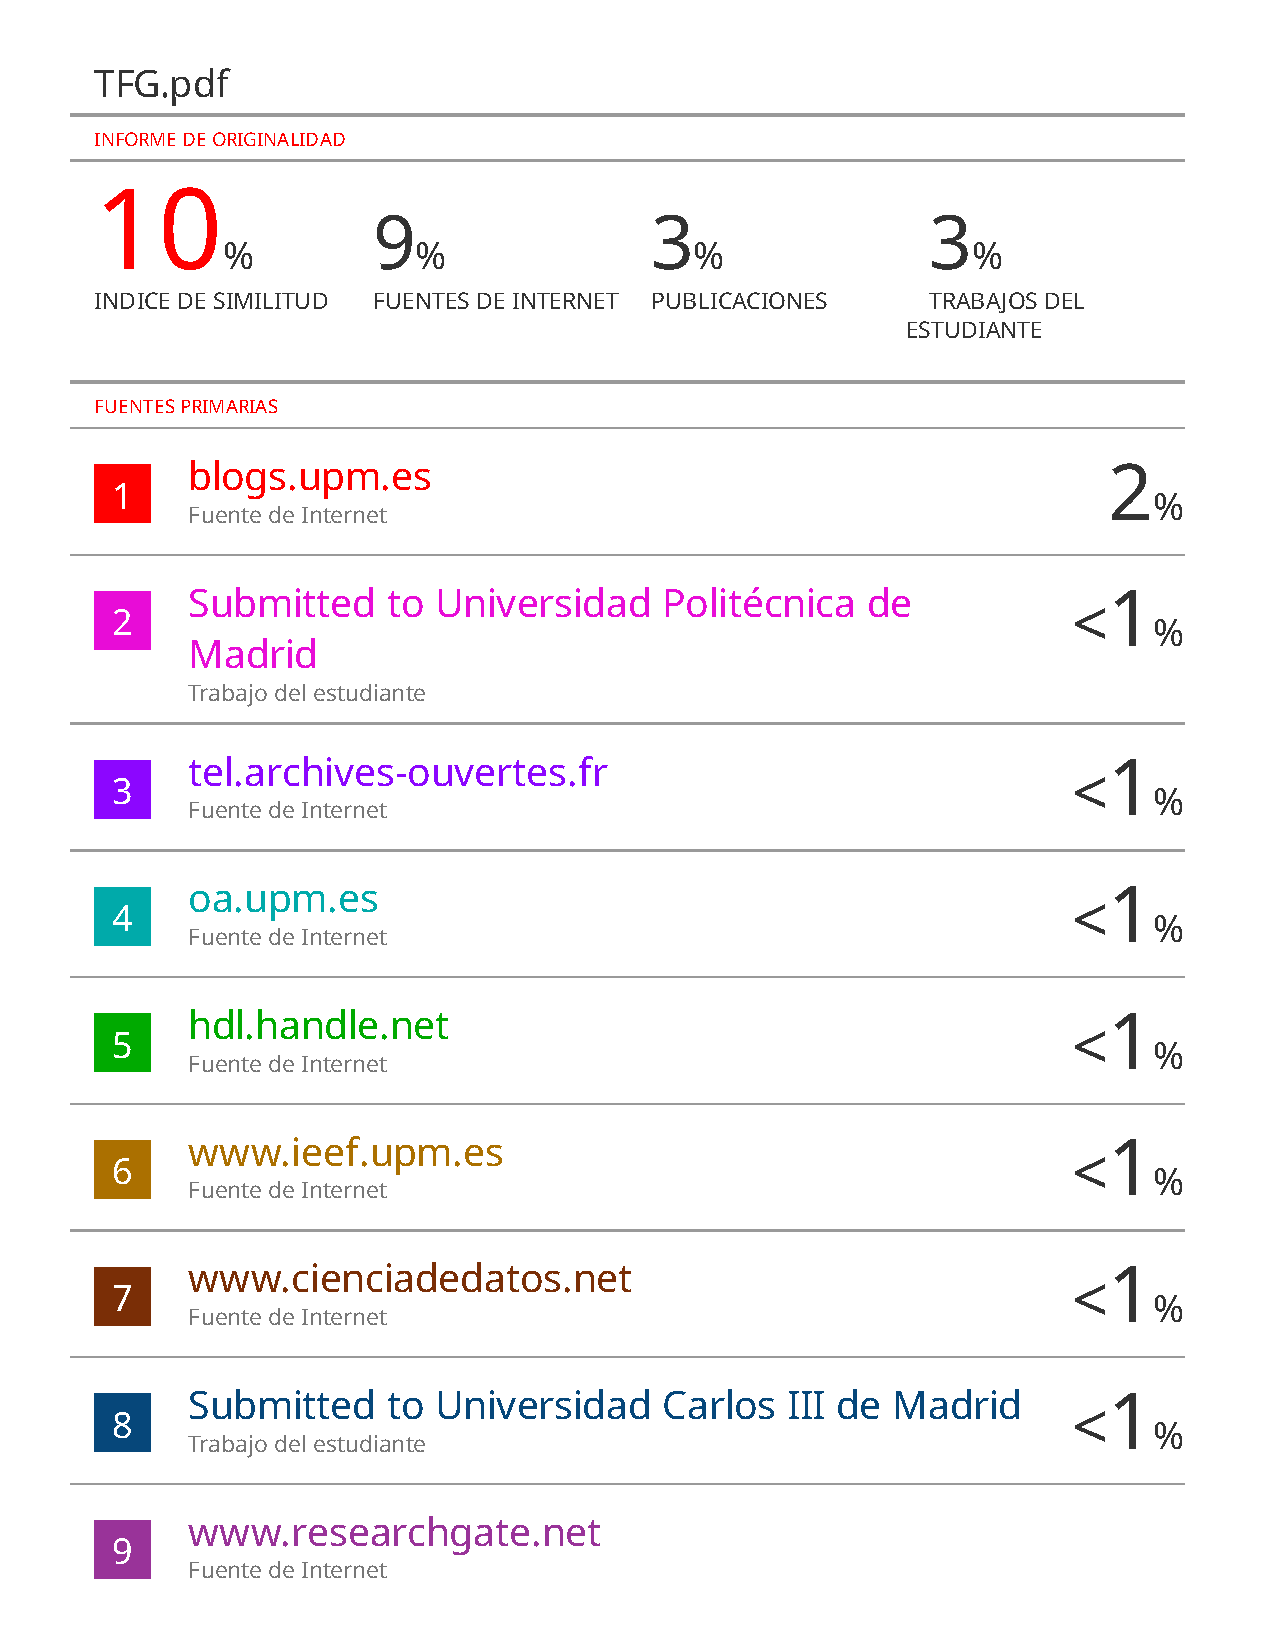
\includepdf[pages=-]{TFG_turnitin_puntuaciones.pdf}




\backmatter
%Glosario, lista de símbolos, notas, etc.



%genera doble hoja en blanco
\cleardoublepage

%apartado de bibliografía
\addcontentsline{toc}{chapter}{Bibliografía}

%estilo de bibliografía: plana, alfa...
\bibliographystyle{unsrt}
%se incluye la bibliografía. Archivo de tipo .bib (bibtex)
\bibliography{bibliografia/bibliografia}

%fin del documento
\end{document}